\documentclass[10pt,conference,letterpaper]{IEEEtran}
\special{papersize=8.5in,11in}
\usepackage{latexsym}
\usepackage{amsfonts}
\usepackage{amsmath}
\usepackage{amssymb}
\usepackage{color}
\usepackage{epsfig}
\usepackage{xspace}
\usepackage{graphicx,epstopdf}
\usepackage{times}
\usepackage{subfigure}
\usepackage{cite}
\usepackage{balance}
\usepackage{amsmath, bm}
\usepackage[english]{babel}
\usepackage{array}

%\pdfpagewidth=8.5in
%\pdfpageheight=11in

% \newenvironment{note}[1]{\medskip\noindent \textbf{#1:}}%
        % {\medskip}

% \newenvironment{proofsketch}{\noindent{\bf Proof Sketch.}}%
        % {\hspace*{\fill}$\Box$\par\vspace{4mm}}
% \newenvironment{proofof}[1]{\smallskip\noindent{\bf Proof of #1.}}%
        % {\hspace*{\fill}$\Box$\par}

% \newcommand{\etc}{{etc.}\xspace}
% \newcommand{\assign}{\leftarrow\xspace}
% \newcommand{\eps}{\epsilon\xspace}

% \newcommand{\ctab}{Table~}
% \newcommand{\csec}{Section~}
% \newcommand{\cthm}{Theorem~}
% \newcommand{\clem}{Lemma~}
% \newcommand{\cequ}{Equation~}
% \newcommand{\cfig}{Figure~}
% \newcommand{\calg}{Algorithm~}
% \newcommand{\cexp}{Example~}

% \newcommand{\opt}{\textrm{\sc OPT}\xspace}
% \newcommand{\script}[1]{\mathcal{#1}\xspace}
% \newcommand{\ceil}[1]{\lceil #1 \rceil\xspace}
% \newcommand{\floor}[1]{\lfloor #1 \rfloor\xspace}

% \newcommand{\pr}[1]{{\bf Pr}\!\left[#1\right]\xspace}
% \newcommand{\bigoh}[1]{{\bf O}\!\left(#1\right)\xspace}
% \newcommand{\reach}[3]{{\bf R}^{#1}_{#2}(#3)\xspace}
% \newcommand{\Nreach}[3]{{\bf \overline{R}}^{#1}_{#2}(#3)\xspace}
% \newcommand{\reachI}[3]{{\bf I}^{#1}_{#2}(#3)\xspace}
% \newcommand{\NreachI}[3]{{\bf \overline{I}}^{#1}_{#2}(#3)\xspace}

% \newcommand{\gset}{{\cal G}\xspace}
% \newcommand{\dfst}{{\rm DFST}\xspace}
% \newcommand{\dfs}{{\rm DFS}\xspace}
% \newcommand{\dfsj}{{\rm JumpDFS}\xspace}

\newcommand{\eat}[1]{}

\newcommand{\eop}{\hspace*{\fill}\mbox{$\Box$}}     % End of proof

\newcommand{\nthesection}{\arabic{section}}
\newcounter{theorem}
\renewcommand{\thetheorem}{\arabic{theorem}}
\newcounter{prop}
\renewcommand{\theprop}{\arabic{theorem}}
\newcounter{property}
\renewcommand{\theprop}{\arabic{theorem}}
\newcounter{lemma}
\renewcommand{\thelemma}{\arabic{theorem}}
\newcounter{cor}
\renewcommand{\thecor}{\arabic{theorem}}
\newcounter{claim}
\renewcommand{\theclaim}{\arabic{theorem}}

\newcommand{\thmspace}{1ex}
\newenvironment{theorem}{\begin{em}
        \refstepcounter{theorem}
        {\vspace{\thmspace} \noindent\bf  Theorem  \thetheorem:}}{
        \end{em}\eop\vspace{\thmspace}} %\hspace*{\fill}\vspace*{1ex}}
\newenvironment{prop}{\begin{em}
        \refstepcounter{theorem}
        {\vspace{\thmspace}\noindent \bf Proposition \theprop:}}{
        \end{em}\eop\vspace{\thmspace}}%\hspace*{\fill}\vspace*{1ex}}

\newcounter{fact}
\newenvironment{fact}{\begin{em}
        \refstepcounter{fact}
        {\vspace{\thmspace}\noindent \bf Fact \arabic{fact}:}}{
        \end{em}\eop\vspace{\thmspace}}%\hspace*{\fill}\vspace*{1ex}}

\newenvironment{lemma}{\begin{em}
        \refstepcounter{theorem}
        {\vspace{\thmspace}\noindent\bf Lemma \thelemma:}}{
        \end{em}\eop\vspace{\thmspace}} %\hspace*{\fill}\vspace*{1ex}}
\newenvironment{cor}{\begin{em}
        \refstepcounter{theorem}
        {\vspace{\thmspace}\noindent\bf Corollary \thecor:}}{
        \end{em}\eop\vspace{\thmspace}} %\hspace*{\fill}\vspace*{1ex}}
\newenvironment{claim}{\begin{em}
        \refstepcounter{theorem}
        {\vspace{\thmspace}\noindent\bf Claim \theclaim:}}{
        \end{em}\eop\vspace{\thmspace}} %\hspace*{\fill}\vspace*{1ex}}

\newcounter{definition}[section]
\renewcommand{\thedefinition}{\nthesection.\arabic{definition}}
\newenvironment{definition}{
        \vspace{1.5ex}
        \refstepcounter{definition}
        {\noindent\bf Definition {\bf \thedefinition}:}}{\eop\vspace{1.5ex}}
\newcounter{alg}[section]
\renewcommand{\thealg}{\nthesection.\arabic{alg}}
\newenvironment{alg}[1]{
        \refstepcounter{alg}
        {\vspace{1ex}\noindent\bf Algorithm \thealg:\, #1}}{
        \vspace*{1ex}}
\newcounter{arule}
\renewcommand{\thearule}{\arabic{arule}}
\newenvironment{arule}{
        \vspace{0.6ex}
        \refstepcounter{arule}
        {\noindent \em Rule \thearule:}}{
        }

%\renewenvironment{proof}{
%\newenvironment{proof}{
%        \vspace{1ex}
%        {\noindent\bf Proof:}}{\eop\vspace{1ex}}
\newenvironment{proofS}{
        \vspace{0ex}
        {\noindent\bf Proof:}}{\eop\vspace{0ex}}
\newenvironment{proofSketch}{
        \vspace{0ex}
        {\noindent\bf Proof Sketch:}}{\eop\vspace{0ex}}
\newenvironment{property}{
        \vspace{1ex}
        {\noindent\bf Property:}}{\eop\vspace{1ex}}

\newcounter{example}
\renewcommand{\theexample}{\arabic{example}}
\newenvironment{example}{
        \vspace{1.5ex}
        \refstepcounter{example}
        {\noindent\bf Example \theexample:}}{
        \eop\vspace{1.5ex}}

\newcommand{\lemmachar}{{\unskip\nobreak\hfil\penalty50\hskip1em\hbox{}%
\nobreak\hfil\rule{1.2ex}{1.4ex}\hfil%
\parfillskip=0pt \finalhyphendemerits=0 \par}}


% ALGORITHMS
%%%%%%%%%%%%%%%%%%%%%%%%%%%%%%%%%%%%%%%%%%%%%%%%%%%%%%%%%%%%%%%%%%%%%%%%%%%%%%%
\newcommand{\SELECT}{\mbox{{\bf select}}\ }
\newcommand{\FROM}{\mbox{{\bf from}\ }}
\newcommand{\WHERE}{\mbox{\bf where}\ }
\newcommand{\SUM}{\mbox{{\bf sum}}\ }
\newcommand{\GROUPBY}{\mbox{{\bf group by}}\ }
\newcommand{\HAVING}{\mbox{{\bf having}}\ }
\newcommand{\CASE}{\mbox{{\bf case}}\ }
\newcommand{\END}{\mbox{{\bf end}}\ }
\newcommand{\WHEN}{\mbox{{\bf when}}\ }
\newcommand{\EXISTS}{\mbox{{\bf exists}}\ }
\newcommand{\COUNT}{\mbox{\kw{count}}}
\newcommand{\INSERTINTO}{\mbox{{\bf insert into}}\ }
\newcommand{\UPDATE}{\mbox{{\bf update}}\ }
\newcommand{\SET}{\mbox{{\bf set}}\ }
\newcommand{\IN}{\mbox{{\bf in}}\ }
\newcommand{\If}{\mbox{\bf if}\ }
\newcommand{\Let}{\mbox{\bf let}\ }
\newcommand{\Call}{\mbox{\bf call}\ }
\newcommand{\Then}{\mbox{\bf then}\ }
\newcommand{\To}{\mbox{\bf to}\ }
\newcommand{\Else}{\mbox{\bf else}\ }
\newcommand{\ElseIf}{\mbox{\bf elseif}\ }

\newcommand{\While}{\mbox{\bf while}\ }
\newcommand{\Begin}{\mbox{\bf begin}\ }
\newcommand{\End}{\mbox{\bf end}\ }
\newcommand{\Do}{\mbox{\bf do}\ }
\newcommand{\Downto}{\mbox{\bf downto}\ }
\newcommand{\Repeat}{\mbox{\bf repeat}\ }
\newcommand{\Until}{\mbox{\bf until}\ }
\newcommand{\For}{\mbox{\bf for}\ }
\newcommand{\Merge}{\mbox{\bf merge}\ }
\newcommand{\Replace}{\mbox{\bf replace}\ }
\newcommand{\Remove}{\mbox{\bf remove}\ }
\newcommand{\Find}{\mbox{\bf find}\ }
\newcommand{\Each}{\mbox{\bf each}\ }

\newcommand{\ForEach}{\mbox{\bf for each}\ }
\newcommand{\Or}{\mbox{\bf or}\ }
\renewcommand{\And}{\mbox{\bf and}\ }
\newcommand{\Not}{\mbox{\bf not}\ }
\newcommand{\Break}{\mbox{\bf break}\ }
\newcommand{\Continue}{\mbox{\bf continue}\xspace}
\newcommand{\Return}{\mbox{\bf return}\ }
\newcommand{\Case}{\mbox{\bf case}\ }
\newcommand{\Of}{\mbox{\bf of}\ }
\newcommand{\EndCase}{\mbox{\bf end-case}\ }
\newcommand{\NIL}{\mbox{\em nil}}
\newcommand{\False}{\mbox{\em false}}
\newcommand{\True}{\mbox{\em true}}
\newcommand{\algAND}{{\sc and}\xspace}
\newcommand{\OR}{{\sc or}\xspace}
\newcommand{\NOT}{{\sc not}\xspace}
%%%%%%%%%%%%%%%%%%%%%%%%%%%%%%%%%%%%%%%%%%%%%%%%%%%%%%%%%%%%%%%%% ALGORITHMS

\newcommand{\spara}[1]{\smallskip\noindent{\bf #1}}
\newcommand{\squishlist}{
 \begin{list}{$\bullet$}
  {  \setlength{\itemsep}{0pt}
     \setlength{\parsep}{3pt}
     \setlength{\topsep}{3pt}
     \setlength{\partopsep}{0pt}
     \setlength{\leftmargin}{2em}
     \setlength{\labelwidth}{1.5em}
     \setlength{\labelsep}{0.5em}
} }
\newcommand{\squishlisttight}{
 \begin{list}{$\bullet$}
  { \setlength{\itemsep}{0pt}
    \setlength{\parsep}{0pt}
    \setlength{\topsep}{0pt}
    \setlength{\partopsep}{0pt}
    \setlength{\leftmargin}{2em}
    \setlength{\labelwidth}{1.5em}
    \setlength{\labelsep}{0.5em}
} }

\newcommand{\squishdesc}{
 \begin{list}{}
  {  \setlength{\itemsep}{0pt}
     \setlength{\parsep}{3pt}
     \setlength{\topsep}{3pt}
     \setlength{\partopsep}{0pt}
     \setlength{\leftmargin}{1em}
     \setlength{\labelwidth}{1.5em}
     \setlength{\labelsep}{0.5em}
} }

\newcommand{\squishend}{
  \end{list}
}
\newcommand{\sttab}{\rule{0pt}{8pt}\\[-3ex]}
\newcounter{ccc}
\newcommand{\bcc}{\setcounter{ccc}{1}\theccc.}
\newcommand{\icc}{\addtocounter{ccc}{1}\theccc.}
\newcommand{\myhrule}{\rule[.5pt]{\hsize}{.5pt}}
\newcommand{\mat}[2]{{\begin{tabbing}\hspace{#1}\=\+\kill #2\end{tabbing}}}
\newcommand{\stitle}[1]{\vspace{0.75ex}\noindent{\bf #1}}
\newcommand{\etitle}[1]{\vspace{0.5ex}\noindent{\em \underline{#1}}}
\newcommand{\marked}[1]{\textcolor{red}{#1}}
\newcommand{\markedb}[1]{\textcolor{blue}{#1}}
\newcommand{\subsubtitle}[1]{\vspace{0.5ex}\noindent\underline{{\bf #1}}}

%\newcommand{\stab}{\rule{0pt}{8pt}\\[-1.6ex]}
%\newcommand{\sttab}{\rule{0pt}{8pt}\\[-2ex]}
\newcommand{\sstab}{\rule{0pt}{8pt}\\[-2ex]}
\newcommand{\bi}{\begin{itemize}}
\newcommand{\ei}{\end{itemize}}

\newcommand{\ie}{\emph{i.e.,}\xspace}
\newcommand{\eg}{\emph{e.g.,}\xspace}
\newcommand{\wrt}{\emph{w.r.t.}\xspace}
\newcommand{\aka}{\emph{a.k.a.}\xspace}
\newcommand{\kw}[1]{{\ensuremath {\mathsf{#1}}}\xspace}

%baselines
\newcommand{\ewpr}{{\sc EWPR}\xspace}
\newcommand{\ewprall}{$\kw{EWPR^*}$}
\newcommand{\blpr}{{\sc PR}\xspace}
\newcommand{\blwpr}{{\sc WPR}\xspace}
\newcommand{\blmulrank}{\kw{MulRank}}

\newcommand{\pagerank}{\kw{PRank}} %PageRank
\newcommand{\futurerank}{\kw{FRank}} %FutureRank
\newcommand{\hhgrank}{\kw{HRank}} %HHGBiRank
\newcommand{\ensemblerank}{\kw{SARank}}
\newcommand{\batensemble}{\kw{batSARank}}
\newcommand{\incensemble}{\kw{incSARank}}
\newcommand{\powensemble}{\kw{powSARank}}

%\newcommand{\twprdag}{{\sc CTWPR}\xspace}
%\newcommand{\inctwprdag}{\kw{inc}{\sc CTWPR}\xspace}
%\newcommand{\powtwprdag}{\kw{pow}{\sc CTWPR}\xspace}

\newcommand{\scc}{{\sc SCC}\xspace}
\newcommand{\sccs}{{\sc SCCs}\xspace}

\newcommand{\twprscc}{\kw{bat}{\sc TWPR}\xspace}
\newcommand{\inctwprscc}{\kw{inc}{\sc TWPR}\xspace}
\newcommand{\powtwprscc}{\kw{pow}{\sc TWPR}\xspace}


\newcommand{\PairAcc}{\kw{PairAcc}}

%dataset
\newcommand{\magdata}{{\sc MAG}\xspace}
\newcommand{\aan}{{\sc AAN}\xspace}
\newcommand{\aminer}{{\sc DBLP}\xspace}
\newcommand{\recom}{{\sc Recom}\xspace}
\newcommand{\fcita}{{\sc PFCtn}\xspace}

\begin{document}


\title{Ensemble Enabled Time-Weighted PageRank}


\title{Scholarly Article Ranking with Ensembles}



\title{Ensemble Enabled Scholarly Article Ranking}

%\title{Dynamic Scholarly Article Ranking with Ensembles}

\title{Query Independent Dynamic Scholarly Article Ranking}

\title{Query Independent Scholarly Article Ranking}


\author{%
% author names are typeset in 11pt, which is the default size in the author block
{Shuai Ma, Chen Gong, Renjun Hu, Dongsheng Luo, Chunming Hu, Jinpeng Huai}%
% add some space between author names and affils
\vspace{1.6mm}\\
%
\fontsize{10}{10}\selectfont\itshape
SKLSDE Lab, Beihang University, Beijing, China\\
Beijing Advanced Innovation Center for Big Data and Brain Computing, Beijing, China\\
%
\fontsize{9}{9}\selectfont\ttfamily\upshape\vspace{0.5ex}
\{mashuai, gongchen, hurenjun, lds1995, hucm, huaijp\}@buaa.edu.cn
}

\eat{
\author{\IEEEauthorblockN{Shuai Ma, Chen Gong, Renjun Hu, Dongsheng Luo, Chunming Hu, Jinpeng Huai\\
{\small SKLSDE Lab, Beihang University, Beijing, China}\\
{\small Beijing Advanced Innovation Center for Big Data and Brain Computing, Beijing, China}\\
{\small \{mashuai, gongchen, hurenjun, lds1995, hucm, huaijp\}@buaa.edu.cn}}
}
}%%%%%%% eat

\eat{
\author{
Shuai Ma, Chen Gong, Renjun Hu, Dongsheng Luo, Chunming Hu, Jinpeng Huai}
\affiliation{%
  \institution{SKLSDE Lab, Beihang University, China}
  \institution{Beijing Advanced Innovation Center for Big Data and Brain Computing, China}
  \institution{\{mashuai, gongchen, hurenjun, lds1995, hucm, huaijp\}@buaa.edu.cn}
  }
}%%%%%%%%% eat

\maketitle


\begin{abstract}
%This paper describes our solution for WSDM Cup 2016.
Ranking query independent scholarly articles is a
%critical and challenging 
practical and difficult task, due to the
heterogeneous, evolving and dynamic nature of entities involved in scholarly articles.
To do this, we first propose a scholarly article ranking model by assembling the importance of involved entities (\eg articles, venues and authors) such that the importance is a combination of {\em prestige} and {\em popularity} to capture the evolving nature of entities.
%To compute the prestige of articles and venues, we propose a novel Time-Weighted PageRank that extends traditional PageRank with a time decaying factor.
To compute the prestige of articles and venues, we propose a novel Time-Weighted PageRank that extends traditional PageRank with a time decaying factor. %( based on the citation statistics.  instead of simple exponential decay).
We then develop a batch algorithm for scholarly article ranking, in which we propose a block-wise method for Time-Weighted PageRank in terms of an analysis of the citation characteristics of scholarly articles. We further develop  an incremental algorithm for dynamic scholarly article ranking, which partitions graphs into {\em affected and unaffected areas}, and employs different updating strategies for nodes in different areas. Using real-life data, we finally conduct an extensive experimental study, and show that our approach is both effective and efficient for ranking scholarly articles.
\end{abstract}



\section{Introduction}
\label{sec-intro}

Query independent ranking of scholarly articles has drawn significant attentions from both academia~\cite{Garfield471,Hirsch15112005,Liang16AAAI,Jiang12-MRank,Waltman2014,Wang16TIST,Ng11KDD,Li08TSRanking,
Wang13AAAI,sayyadi09,WalkerXKM07} and industry~\cite{g-scholar,Sinha15:MAG,sem-scholar}.
Generally speaking, a ranking is {\em a function that assigns each item a numerical score}. Query independent ranking aims to give a static ranking based on the scholarly  data only, and is independent of how well articles match a specific query. Such a ranking plays a key role in literature recommendation systems, especially in the {\em cold start} scenario.
%,TanLMGSW16

In the academia, popular approaches have witnessed a shift from citation-count analysis~\cite{Garfield471,Hirsch15112005} to graph analysis~\cite{Liang16AAAI,Jiang12-MRank,Waltman2014,Wang16TIST,Ng11KDD,Li08TSRanking,Wang13AAAI,sayyadi09,WalkerXKM07}, as graph-based methods further leverage the global or local structure of bibliographic networks and  the interactions among heterogeneous entities, and, hence, are typically more appropriate.
%
Efforts have also been made from the industry. Google Scholar~\cite{g-scholar} aims to rank articles in the way researchers do, weighing the full text, where they were published, who they were written by, as well as how often and how recently they have been cited; Microsoft Academic~\cite{Sinha15:MAG} considers how often and to which a publication is cited to determine the ranking; And
Semantic Scholar~\cite{sem-scholar} proposes to use the citation velocity, which is a weighted average number of article citations in the last three years.


% Zhou07-CoRank,
% from citation-count analysis~\cite{Garfield471,Hirsch15112005}
% https://scholar.google.com/intl/zh-CN/scholar/about.html
% http://academic.research.microsoft.com/About/Help.htm
% https://www.semanticscholar.org/faq#citation-velocity


Scholarly articles are involved with multiple entities such as authors, venues, dates and references. That is, scholarly article ranking is essentially a problem of assessing the importance of nodes in a heterogeneous network.
However, effective and efficient ranking of nodes in such a large complex network is a difficult task due to the heterogeneous, evolving and dynamic natures of involved entities~\cite{AggarwalS14-survey,fcs-biggraph}.

First, even if we are only to rank one type of entities (\ie scholarly articles), the other types of entities (\eg venues and authors) are closely involved, and, moreover, different types of entities may have different impacts on the ranking of scholarly articles.
%
Second, the importance of articles evolves with time in a complex manner~\cite{WangSB13,Chakraborty15}.
%Newly published articles are very likely to have increasing impacts in the next few years, and those published many years ago tend to have decreasing impacts, as researchers potentially have more interests in recently reported results. Indeed, as shown by the statistics of three scholarly datasets (\aan, \aminer and \magdata) in Fig.~\ref{fig-citation}, the citation numbers of articles in general reach the peak in the first 1 or 2 years after their publication, and then decrease accordingly. % Note that we do not plot the proportion of citations at $x=0$ on \aminer, which is an impractical value of 23.6\%. The above citation pattern is described as a complex log-normal probability in~\cite{WangSB13}.
Newly published articles are very likely to have increasing impacts in the next few years, and those published many years ago tend to have decreasing impacts, which conforms to the universal citation pattern of articles such that the number of citations generally grows in the first two to three years, and then declines in the following years~\cite{Chakraborty15}. In addition to the universal one, individual articles indeed follow a diverse set of patterns featured by the peak time of the number of citations~\cite{Chakraborty15}.
Finally, academic data is dynamic and continuously growing. Indeed, the number of articles in Microsoft Academic Graph has exceeded 126 million, and keeps increasing at around 5.7 million per year~\cite{Sinha15:MAG}. This may cause certain long-term biases into data, \eg the number of citations increases significantly over time~\cite{BornmannM15}, which should be properly considered for scholarly article ranking.


Query independent ranking of scholarly articles remains challenging~\cite{wsdmcup}, although there exists quite a bit of work on scholarly article ranking, \eg~\cite{Garfield471,Liang16AAAI,Jiang12-MRank,Waltman2014}.
Most previous work exploits the time-dependent information of scholarly data in the form of exponential decay~\cite{Li08TSRanking,Wang13AAAI,sayyadi09,WalkerXKM07}, which fails to capture the diverse citation patterns of individual articles~\cite{Chakraborty15}.
Further, to our knowledge, little concern has been paid to dynamic scholarly article ranking except \cite{GhoshKHLL11} with a strong and impractical assumption that there are no citations between articles published in the same years.
%\marked{Finally, the bias caused by the dynamic nature of data has never been exploited in scholarly article ranking}.




\stitle{Contributions \& Roadmap}.
To this end, we propose an effective and efficient approach for query independent scholarly article ranking in a dynamic environment.

\sstab(1) We first  propose a \underline{S}cholarly \underline{A}rticle \underline{Rank}ing model, referred to as \ensemblerank, by assembling the importance of three classes of entities (articles, venues and authors) for scholarly article ranking (Section \ref{sec-model}).
%
The importance is a combination of {\em prestige} and {\em popularity} to capture the evolving nature of entities.
%
To compute the prestige of articles and venues, we propose a novel {\em Time-Weighted PageRank} with a time decaying factor based on the citation statistics (instead of simple exponential decay), and the prestige of authors is the average prestige of all their published articles.
%
The popularity of an article is the sum of all its citation freshness (closeness to the current year), while the one of venues and authors is the average popularity of their associated articles.
%
%Observe that (a), intuitively, prestige favors articles with many citations soon after their publication, and popularity favors those with recent citations, and (b) both prestige and popularity capture the evolving nature of entities.
%
To our knowledge, our Time-Weighted PageRank is among the first to incorporate diverse citation patterns of individual articles and to exploit citation statistics for scholarly article ranking.
%and the long-term bias caused by the dynamic nature of data

\sstab(2)  We then develop  a batch algorithm for scholarly article ranking (Section \ref{sec-alg}), in which we propose a block-wise method for Time-Weighted PageRank %\markedb{and show its efficiency advantage in terms of an analysis of the citation characteristics and a specific structural property of scholarly graphs.}
%in which we propose a block-wise method for Time-Weighted PageRank
in terms of an analysis of the citation characteristics of scholarly articles.

\sstab(3)
We further develop an incremental algorithm for the block-wise algorithm
to deal with dynamic scholarly article ranking (Section~\ref{sec-incAlg}), which partitions graphs into  {\em affected and unaffected areas}, and employs different updating strategies for nodes in affected and unaffected areas.


\sstab(4) Using three real-life scholarly datasets (\aan, \aminer and \magdata) and two sets of ground-truth (\recom and \fcita), we finally conduct an extensive experimental study (Section~\ref{sec-exp}).
(a) We find that our model \ensemblerank improves the pairwise accuracy \cite{Richardson06:BPR} over (\pagerank \cite{Brin98:PageRank}, \futurerank \cite{sayyadi09}, \hhgrank \cite{Liang16AAAI}) by
(13.5\%, 6.8\%, 4.8\%) and (12.0\%, 3.0\%, 3.2\%) \wrt\ \recom and \fcita  on \aan,
(12.7\%, 5.0\%, 4.9\%) and (14.0\%, 6.5\%, 4.6\%) \wrt\ \recom and \fcita on \aminer, and
(6.5\%, 2.5\%, 2.2\%) and (13.4\%, 6.0\%, 2.4\%) \wrt\ \recom and \fcita on \magdata, on average, respectively.
%
(b) Our batch algorithm \batensemble and incremental algorithm \incensemble are also efficient. Indeed, \incensemble is on average (1.7, 2.8, 116) and (2.0, 4.4, 245) times faster than (\batensemble, \futurerank, \hhgrank)  on the large \aminer and \magdata, respectively.
%%%%%%%%%%%%%%%%%%%%%%%%%
\eat{
All the detailed proofs can be found in \cite{SARank-full}.
%All the proofs can be found in \cite{SARank-full}.
}
\eat{
\stitle{Organization}. The rest of our paper is organized as follows. The latter part of Section~\ref{sec-intro} summarizes related work. Section~\ref{sec-model} introduces the ranking model. Section~\ref{sec-alg} .... Section~\ref{sec-incAlg} .... Experimental results are reported in Section~\ref{sec-exp}, followed by conclusions in Section~\ref{sec-conc}.
}




\section{Ranking Model}
\label{sec-model}

In this section, we first present Time-Weighted PageRank for evaluating  the importance of entities, defined as a combination of the prestige and popularity, and then introduce our ranking model \ensemblerank that assembles the importance of articles, venues and authors involved in scholarly articles.

%It further assembles the importance of heterogeneous entities involved to rank scholarly articles.
%The model is based on PageRank~\cite{Brin98:PageRank}, which was initially designed for web pages and widely applied to many other tasks, including article ranking~\cite{Li08TSRanking,Richardson06:BPR,sayyadi09,Zhou07-CoRank}.


\subsection{Time-Weighted PageRank}
\label{subsec-twpr}

We first present Time-Weighted PageRank (TWPageRank) based on citation statistics, as the direct use of PageRank for ranking scholarly articles is problematic as discussed below.




%PageRank~\cite{Brin98:PageRank} has been extensively applied to the ranking of scholarly articles~\cite{Waltman2014,sayyadi09,Zhou07-CoRank,ChenXMR07}, as hyperlinks among Web pages can be easily replaced with citation relationships among articles, and citation analysis plays a key role to evaluate the importance of scholarly articles. However,



\noindent(1) Different articles typically have different impacts in practice, and there is a need to differentiate, while PageRank essentially assumes equal impacts.

%, such that each article can distribute more of its authority to those that are more influential to it.

\noindent(2) The semantics of citation relationships are time-dependent, which means that citations at different periods of time may reveal different information. Note that this has already been exploited for scholarly article ranking~\cite{Li08TSRanking,Wang13AAAI,WalkerXKM07}, while PageRank does not consider this temporal factor at all.
% and each individual article reaches their periods in different time

\stitle{Time-Weighted PageRank (TWPageRank)}. Most previous work simply exploits temporal information in the form of exponential decay~\cite{Li08TSRanking,Wang13AAAI,sayyadi09,WalkerXKM07}. We rethink the usage of time information in terms of the impacts of scholarly articles.
Recall that articles are categorized  into six citation patterns featured by the time when the articles reach their citation peaks~\cite{Chakraborty15}: (a) {\em PeakInit} with the citation-count peak in the first five years (but not the first year) after publication, (b) {\em PeakMul} with distinct multiple peaks, (c) {\em PeakLate} with a single peak in at least five years after publication, (d) {\em MonDec} with monotonically decreasing citations, (e) {\em MonIncr} with monotonically increasing citations, and, (f) {\em Other} for articles whose average numbers of citations per year are less than 1. Though the number of citations is an indicator of the impacts of articles~\cite{WangSB13,Garfield471}, its impact is time-dependent and is not simply in the form of exponential decay.
In general, {\em the impact of an article tends to decay with time after the peak time only}. That is, the impacts of articles directly decay with time only for those in {\em MonDec}, and decay with time after the peak time for those in {\em PeakInit}, {\em PeakLate} and {\em PeakMul}, and do not decay for ones in {\em MonIncr} (which is rare).
%Otherwise, its impact is fixed as a constant number. %, since we argue that the increment of its citations during this period is mainly due to the increase of its popularity.
Also observe that {\em each individual article has its own peak time} as articles may reach their citation peaks in different patterns and time.
%using the peak year in Fig.~\ref{fig-citation} is not appropriate for all articles. On the contrary, we compute a peak year for each article.


\eat{
 the proportion of total citations \wrt the number of years after publication.
%Here we use the number of citations to evaluate the impacts of articles.
\marked{As we can see, the number of citations reaches a peak in the first 1 or 2 years, and gradually decreases after that, which also conforms to our perception of the impacts of articles~\cite{WangSB13}. Note that the peak time differs from one dataset to another.}


According to Fig.~\ref{fig-citation}, the impact of an article does depend on time, but not simply in the form of exponential decay. Specifically, if an article is cited after the citation peak, its impact should decay with time. Otherwise, its impact is fixed as a constant number. %, since we argue that the increment of its citations during this period is mainly due to the increase of its popularity.
Moreover, considering that articles might reach their citation peaks in different time, we compute {\em the peak time for each individual article}, rather than using the same citation peak for all articles.
%using the peak year in Fig.~\ref{fig-citation} is not appropriate for all articles. On the contrary, we compute a peak year for each article.
}

\begin{figure}
\centering
\includegraphics[scale=0.48]{fig/yearly-references.eps}
\vspace{-1ex}
\caption{\small Citation statistics of scholarly articles that reports the (logscale) percentage of the number of citations of each year \wrt\ the total number of citations  in  \aan, \aminer and \magdata, respectively.}
\label{fig-reference}
\vspace{-3ex}
\end{figure}


Based on the above discussion, we propose TWPageRank that evaluates the prestige of nodes (\eg scholarly articles) in a directed graph, such that each node is attached with time information. It differs from PageRank by weighting the influence propagation using the {\em impact weights on edges}, which represent the relative amounts of time-dependent prestige that should be propagated from the edge sources to targets.
%
Formally, the impact weight on a directed edge $(u,v)$, \ie an edge from $u$ to $v$, is defined as:

\vspace{-1ex}
\begin{small}
\begin{equation} \label{eq-infl-weights}
w(u,v)  =  \begin{cases}  \hspace{7ex} 1 & T_u <  Peak_v \\
  e^{\sigma(T_u-Peak_v)} & T_u \geq Peak_v,
\end{cases}
\end{equation}
\end{small}
%
\noindent where $T_u$ is the time of node $u$, $Peak_v$ is the peak time of node $v$ after which the impact weights of edges to $v$ decay with time, and $\sigma$ is a negative number controlling the decaying speed of the impacts.
By default, Eq.~(\ref{eq-infl-weights}) uses years as its time granularity. Note that the time decaying factor $\sigma$ is introduced to provide flexibility for TWPageRank in various applications, and its value is typically within a small interval, \eg $[-2,0]$, such that $w(u,v)$ does not decay when $\sigma=0$ and already decays more than a half per year when $\sigma=-1$.
For the sake of completeness, we further set $w(u,v)$ to $0$ if there does not exist an edge from $u$ to $v$ in the graph.


For scholarly article ranking, $T_u$ is the publication time of article $u$ and $Peak_v$ should be ideally set to the time when article $v$ has the highest impacts. Basically, it could simply be the year when article $v$ obtains the largest number of citations. However, recent work reveals that the volume of scientific publications as well as the number of citations grow exponentially with time~\cite{Dong2017KDD,BornmannM15}. We also collect and report the citations statistics on three scholarly datasets in Fig.~\ref{fig-reference}, which verifies the exponential distribution. Hence, we adopt the {\em scaled} number of citations $\Psi_v^{(t)}=\Phi_v^{(t)} / \log Z^{(t)}$ such that $\Phi_v^{(t)}$ and $Z^{(t)}$ are the number of citations of article $v$ at year $t$ and the total number of references at year $t$, respectively. The peak time $Peak_v$ is the time that maximizes $\Psi_v^{(t)}$.
%(\aan, \aminer and \magdata)
% since scholarly data is dynamic and continuously growing
%, and the increased number of references of each article over time
%Recent work observes that the volume of scientific publications doubled every 12 years between 1900 and 2015~\cite{Dong2017KDD}. It is not surprising that the number of references also grows exponentially~\cite{BornmannM15}.



The update rule of TWPageRank is:

\vspace{-1ex}
\begin{small}
\begin{equation}\label{eq-twpr}
PR(v)=d\sum_{(u,v)\in E} \frac{w(u,v)PR(u)}{W(u)}+\frac{1-d}{n},
\end{equation}
\end{small}
%
\noindent where $PR(u)$ and $PR(v)$ are the TWPageRank scores of $u$ and $v$, respectively, $E$ is the set of edges, $W(u)=\Sigma_{v} w(u,v)$ is the sum of the impact weights on all edges from $u$, $n$ is the number of nodes and $d$ is a damping parameter in $(0, 1)$. By Eq.~(\ref{eq-twpr}), we can see that prestige is based on the impact weights, not equally distributed.

% in Eq.~(\ref{eq-twpr}) into
Correspondingly, the matrix form of the update rule is:

\vspace{-1ex}
\begin{small}
\begin{equation}
\label{eq-twpr-update}
PR^{(t)}=d M^T  PR^{(t-1)} + (1-d) e/n.
\end{equation}
\end{small}
%
\noindent
Here $PR^{(k)}$ is the TWPageRank vectors after $k$ iterations,  $M$ is the transition matrix such that $M_{u,v}=w(u,v)/W(u)$ and  $e$ is an $n$-dimensional all-one vector $[1]_{n\times1}$.

%We next present the convergence  of TWPageRank as follows.
The linear system in Eq.~(\ref{eq-twpr-update}) is equivalent to {\em irreducible} and {\em aperiodic} Markov chains~\cite{CorsoGR05}, which guarantees the following.


\begin{prop}
\label{prop-converg}
TWPageRank converges to a unique  vector on any graph, regardless of the initial vector.
\end{prop}

\eat{
\begin{proof}
It is known that a sequence of vectors $x^{(k)}$ such that $x^{(k+1)}=A\cdot x^{(k)}+b$ (where $k=0,1,\dots$) converges to a unique vector $x^*$,  regardless of the initial vector $x^0$, if and only if $\rho(A)<1$~\cite{kelley1999iterative}, where $\rho(A)$ is the spectral radius of matrix $A$. Hence, it suffices to show $\rho(d\cdot M^T) < 1$ by Eq.~(\ref{eq-twpr-update}).

As the column sums of $d\cdot M^T$ are all less than or equal to $d$, $||d\cdot M^T||_1 \le d$ where $||d\cdot M^T||_1$ is the 1-norm of matrix $d\cdot M^T$ and is defined as the maximum absolute column sum of $d\cdot M^T$.
We then have $\rho(d\cdot M^T) \le ||d\cdot M^T||_1 \le d < 1$, as the spectral radius of a matrix is always no more than its consistent matrix norms~\cite{spe-radius}, \eg $||\cdot||_1$, which gives the conclusion.
\end{proof}
}

%\stitle{Remarks}. Note that Eq.~(\ref{eq-twpr}) is indeed a general update rule of Weighted PageRank~\cite{Xing04:WPR,Ding11}, and the name of Time-Weighted PageRank comes from the use of time information of citations in the initial impact weight  $w(u,v)$ of Eq.~(\ref{eq-infl-weights}).



\vspace{-1ex}
\subsection{Ranking with Importance Assembling}
\label{subsec-ensemble}


%In our model, the importance of scholarly articles is defined as a combination of the prestige and popularity of its associated articles, venues and authors. Intuitively, prestige favors those with many citations soon after the publication of articles for citation component or associated articles for venue and author components, and popularity favors those with recent citations. Both prestige and popularity capture the temporal nature of entities in scholarly data.
In our model, the importance is defined as a combination of the prestige and popularity. Intuitively, prestige favors those with many citations soon after the publication of articles or associated articles of venues and authors, and popularity favors those with recent citations. Both prestige and popularity capture the temporal nature of entities. %in scholarly data.

Our ranking model \ensemblerank,  illustrated in Fig.~\ref{fig-rankmodel}, assembles the importance of article, venue and author entities for scholarly article ranking, which is computed by the citation, venue and author components, respectively.
%
We next introduce the details of the three components.


\stitle{Citation component}.
The first component computes the importance of articles using the citation information.

A {\em citation graph} $G^c(V^c, E^c)$ is firstly constructed using the citation information such that (a) a node in $V^c$ denotes an article, (b) a directed edge $(u,v)$ in $E^c$ denotes that $u$ cites $v$, and (c) each node is associated with two types of time information: the publication year and the latest year having the largest number of citations.


\sstab(1) The prestige of articles is derived by applying TWPageRank on the citation graph $G^c$, and each article $v$ is assigned the corresponding TWPageRank score as its prestige $Prs_c(v)$.

\sstab(2)  The popularity of an article is the sum of all its citations' freshness, \ie the closeness to the current year:

\vspace{-1ex}
\begin{small}
\begin{equation}\label{eq-pop}
Pop_c(v) = \sum_{{(u,v)\in E^c}} {e^{\sigma (T_0-T_u)}}.
\end{equation}
\end{small}
\noindent
Here $T_0$ is the current year, \ie the latest $T_u$ among all articles in $V^c$, $\sigma$ is the negative decaying factor used in Eq.~(\ref{eq-infl-weights}), and $e^{\sigma (T_0-T_u)}$ represents the freshness of citation $(u,v)$.

%Alternatively, one may want to define $Pop_c(v) = e^{\sigma \cdot (T_0-T_v)}$, \ie decaying with the publication year $T_v$ of article $v$ directly~\cite{sayyadi09,WalkerXKM07}. We propose to use the publication years $T_u$ of citations, instead of $T_v$, since $T_u$ reflects the ages of articles to some extent, \eg articles are probably cited in the next few years after publication(Fig.~\ref{fig-citation}).

Intuitively, the more recent citations an article has, the higher its popularity is, no matter how long it has been published.
Here popularity is introduced to capture the recent importance of articles, and articles with more recent citations have higher popularity scores. %, which is somehow biased to recent articles. Hence, we do not explicitly handle the bias for popularity computation.
%
%\marked{Different from $Peak_v$ in Eq.~(\ref{eq-infl-weights}), the bias of references has little impacts on the popularity. Moreover, the motivation of popularity is to assign higher ranks to articles of recent attention, which is somehow biased to recent articles. Hence, we do not explicitly handle the bias for popularity computation.}
%
Note that the popularity is also normalized such that the sum of  all articles is equal to $1$, similar to the prestige produced by TWPageRank.

\sstab(3) The prestige and popularity are finally combined to produce the importance of articles. Intuitively, an important article is both prestigious and popular. Hence, the {\em citation importance score} $Imp_c(v)$ of an article is defined as a weighted combination of its prestige and popularity:

\vspace{-1ex}
\begin{small}
\begin{equation}\label{eq-imp}
%Imp_c(v) = \sqrt{Prs_c(v) \cdot Pop_c(v)}.
Imp_c(v) = Prs_c(v)^\lambda Pop_c(v)^{1-\lambda},
\end{equation}
\end{small}
\noindent where $\lambda \in [0,1]$ is the importance weighting factor.
The rationales behind Eq.~(\ref{eq-imp}) are as follows. (a) Prestigious articles with many recent citations are ranked at the top, as researchers are very willing to find them; (b) Prestigious articles with rare current citations are ranked lower, as researchers may lose interests in these old articles; And (c) articles with many recent citations are ranked higher, as researchers have potential interests in those of recent attention.

%Here the prestige and popularity are equally weighted to produce the importance of an article, as we focus on query independent ranking. They may be properly weighted when the query information is available, which is beyond the scope of this work.


\begin{figure}[tb!]
\centering
%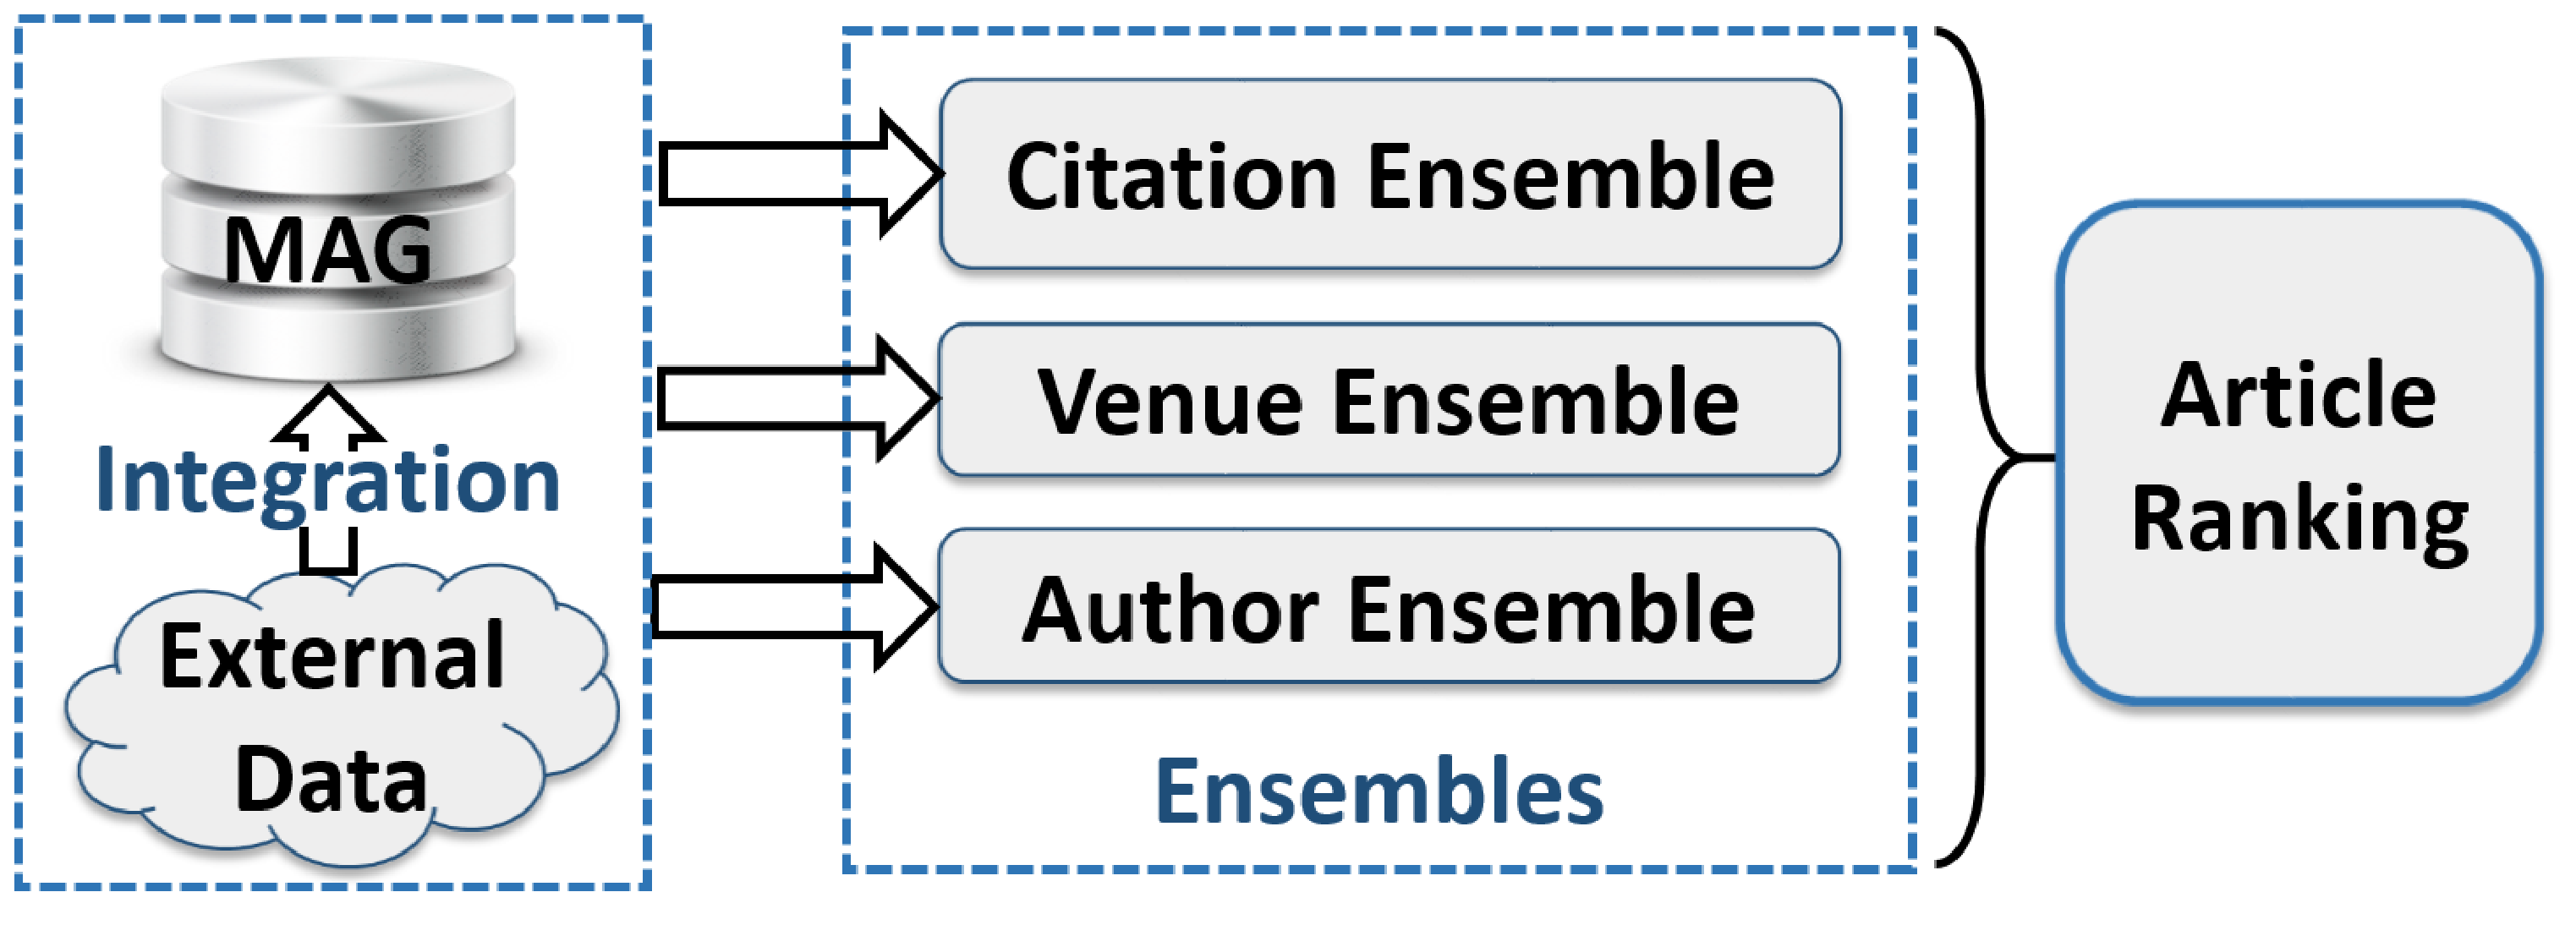
\includegraphics[scale=0.15]{fig/framework.eps}
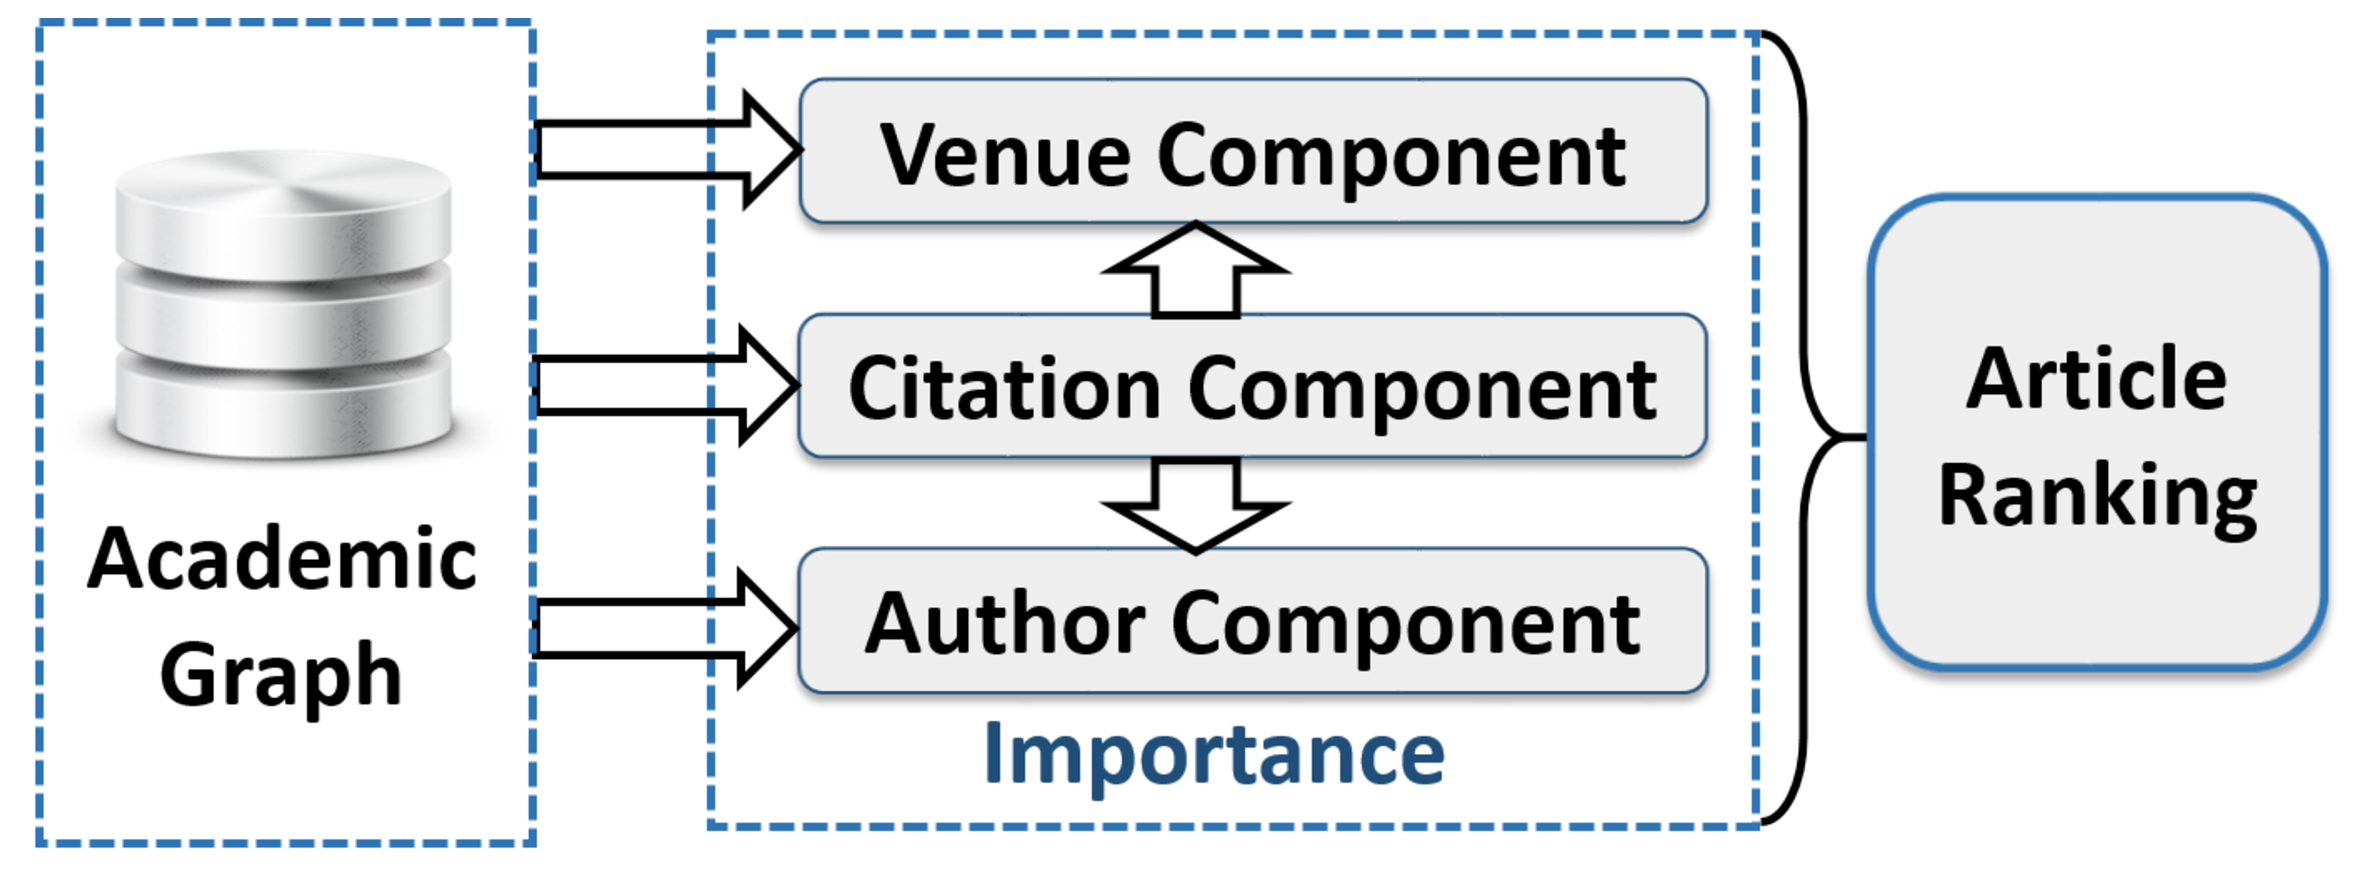
\includegraphics[scale=0.16]{fig/framework-lite-2.eps}
\vspace{-1ex}
\caption{\small Ranking model \ensemblerank} \label{fig-rankmodel}
\vspace{-3ex}
\end{figure}

\stitle{Venue component}.
The second component computes the importance of venues with their associated articles. As the importance of a venue  evolves with time, we treat the venue in each year individually, and its importance is the sum of importance in all individual years.


A {\em venue graph} $G^v(V^v, E^v)$ is firstly constructed using the citation information among venues such that (a) a node in $V^v$ represents a venue in a specific year, (b) a direct edge $(s,t)$ in $E^v$ denotes that there exist articles published in venue (in a specific year) $s$ citing articles published in venue (in a specific year) $t$, and (c) we use the {\em impact weight} to denote the weight $w_v(s,t)$ from venues $s$ to $t$, which is the sum of the impact weights from articles published in $s$ to $t$, \ie

\vspace{-1ex}
\begin{small}
\begin{equation} \label{eq-infl-weights-v}
w_v(s,t)  = \sum_{u\in C(s), v\in C(t)} w(u,v).
\end{equation}
\end{small}
\noindent
Here, $C(s)$ and $C(t)$ are the sets of articles published in $s$ and $t$, respectively, and $w(u,v)$ is the impact weight of edge $(u, v)$ produced in the citation component.

The prestige of a venue in a specific year is computed using the impact weights and the update rule in Eq.~(\ref{eq-twpr}), and the popularity of a venue in a specific year is defined as the average popularity of its articles. The prestige and popularity are combined to derive the importance of a venue in a specific year in the same way as the citation component. Finally, the importance of a venue is treated as the {\em venue importance score} for all articles published in this venue.






\stitle{Author component}.
The author component computes the importance of authors with their published articles.
%
Similar to the venue component, we evaluate the importance of each author, and compute the average importance of the authors of an article as its {\em author importance score}.

However, the resulting author citation graph to compute the prestige is typically too large to handle. Hence, we evaluate the prestige of an author, by using the average prestige of all articles published by the author. Similar to the venue component, the popularity of an author is also defined as the average popularity of her/his published articles. Finally, the prestige and popularity are combined to derive the importance in the same way as the citation component.

%, which can be directly obtained from the citation component,
%to evaluate the authority of that author.

\eat{
\stitle{Affiliation ensemble}.
Recall that articles in our data are also associated with affiliation information. Following the way of the venue or author ensemble, we can derive another ensemble, \ie affiliation ensemble. However, we argue that the use of affiliation ensemble may have negative effects since the correlation between the importance of an article and the average authority of its affiliation(s) is not as strong as others such like authors and venues. As shown by the experimental study in Section~\ref{sec-exp},  the incorporation of the affiliation ensemble impairs the ranking accuracy. Hence, we choose not to use the affiliation ensemble in our model.
}



%\subsection{Ranking with Importance}
%{\label{subsec-eerank}}


\stitle{Ranking with importance assembling}. The aforementioned importance is finally assembled to produce the final ranking, as illustrated in Fig.~\ref{fig-rankmodel}. Before assembling, each component is properly scaled such that the average citation importance score, venue importance score and author importance score
are the same.  Let the scaled importance scores of article $v$ be $R_c(v)$, $R_v(v)$, and $R_a(v)$ from the citation, venue and author components, respectively. The final ranking score $R(v)$ of an article $v$ is aggregated as follows:

\vspace{-1ex}
\begin{small}
\begin{equation} \label{eq-ensemble}
R(v) =  \alpha R_c(v) + \beta R_v(v) + (1 - \alpha - \beta) R_a(v).
\end{equation}
\end{small}
\noindent Here aggregating parameters $\alpha$ and $\beta$ and value $(1 - \alpha - \beta)$ regularize the contributions of the citation, venue and author information. Intuitively, these parameters indicate the intensity of the correlation between the importance of scholarly articles and the specific information.


\stitle{Remark}. This work follows the graph-based formalization, and further develops efficient batch and incremental algorithms based on graphs for scholarly article ranking (Sections~\ref{sec-alg} \& \ref{sec-incAlg}). However, it is also possible to learn a discriminative model that directly optimizes certain loss functions for ranking, similar to \cite{Richardson06:BPR} for ranking Web pages.

%\subsection{Framework}
%\label{subsec-framework}

%Our ensemble enabled ranking model~\ensemblerank is illustrated in Fig.~\ref{fig-rankmodel}, which contains three distinct ensembles derived from academic graph data, \ie the citation ensemble, venue ensemble and author ensemble. The citation ensemble directly uses TWPageRank, while the other two are partially based on TWPageRank. Moreover, the citation ensemble also helps to derive the venue ensemble and author ensemble. These ensembles are further assembled to produce the final ranking.


%As illustrated in Fig.~\ref{fig-rankmodel}, external data is also exploited in \ewpr. How to collect and use external data will be introduced in the coming section.


\eat{
\stitle{Remarks}.
Traditional PageRank equally distributes the prestige of nodes, and PageRank based models suffer from the problem that older articles are preferred since they have accumulated a large number of citations~\cite{Li08TSRanking}, and TWPageRank based models alleviate the problem to a certain degree by lowering the impact weights of articles when they are cited after their peak time, \ie $T_u\geq Peak_v$. We further propose the venue and author ensembles to improve the ranking accuracy.
}



%\stitle{Remarks}.
%Recall that articles in our data are also associated with affiliation information. Following the way of the venue or author ensemble, we can derive another ensemble, \ie affiliation ensemble. However, we argue that the use of affiliation ensemble may have negative effects since the correlation between the importance of an article and the average authority of its affiliation(s) is not as strong as others such like authors and venues. As shown by the experimental study in Section~\ref{sec-exp},  the incorporation of the affiliation ensemble impairs the ranking accuracy. Hence, we choose not to use the affiliation ensemble in our model.


%our method used for author ensemble is both lightweight and effective, as will be shown in the experimental study.

%Two methods are used to evaluate the authority of venues and authors, respectively. We point out that the ensembles are quite flexible to the selection of these methods, and others may also be incorporated in the ensembles if appropriate.

\eat{
\subsection{Dealing with Missing Data}
\label{subsec-impl}

Data quality is one of the most challenging issues in large scale data management, especially for data from open domains and multiple sources, \eg the Microsoft Academic Graph (MAG)~\cite{Sinha15:MAG}.
The early version of MAG has $120$ million scholarly articles, among which we find that there are about $73$ million articles without references and about $77$ million ones without venues. The ranks of those articles with missing information are underestimated by our model \ewpr, since ensembles assign the minimum scores to articles. As a result, data missing seriously impairs the ranking accuracy.

As for references and venues, the later are easier to obtain, and each filled venue can have a direct and substantial impact on the article ranking, \ie $R_v(u)$ of Eq.~(\ref{eq-ensemble}). In contrast, a filled reference only has an indirect and slight impact. Hence, we decide to use external data to fill in missing venues.


%\subsection{Data Collecting}
%\label{subsec-datacraw}
\stitle{Data collecting}.
The raw external data is collected from publicly available Digital Libraries, such as IEEE Xplore ({\footnotesize http://ieeexplo-re.ieee.org/gateway/}),  PubMed ({\footnotesize http://www.ncbi.nlm.nih.gov/pub-med/}) and DBLP ({\footnotesize http://dblp.uni-trier.de/db/}). In total, we collect $2.8$ million articles with venue information as our external data, in which there are $57,000$ different venues.



%\subsection{Data Preprocessing}
%\label{subsec-dataprep}
\stitle{Data preprocessing}.
The venues in MAG are well processed, and are replaced by their series names. For example, {\em ``9th International Conference on Web Search and Data Mining, 2016''} is replaced with {\em ``Web Search and Data Mining''}. This makes it hard to directly link with the collected raw venue names. Hence, we preprocess raw venue names for the simplification of subsequent venue linking.
%
We first remove stop words such as {``on''} and common words like {``Conference''}, as well as years and some special characters from collected raw venue names. Then the same venues are merged, and the number of different venue names is reduced to $42,000$.

%\subsection{Data Linking}
%\label{subsec-datamap}
\stitle{Data linking}.
The final and also the most important step of filling missing venue information is to link each collected venue name to an existing one in MAG. Intuitively, linking based on name similarity is the most effective way such that two venues are linked if their names bear high similarity. We exploit the Jaro metric to evaluate the name similarity, which is based on the number and order of the common characters between two strings, and obtains good results in tasks such as record linkage and name matching~\cite{Cohen03strcompa}. Formally, a collected venue name is linked to an existing one in MAG if their Jaro similarity exceeds a pre-define threshold.

However, such a threshold is nontrivial to determine in practice. A high threshold can guarantee the accuracy of linked pairs, while only a tiny proportion of collected venue names are linked. On the other hand, a low threshold increases the number of linked pairs, which, in the same time, also introduces many errors. In order to reach a good balance between the number of linked pairs and the accuracy, we propose to combine another constraint on topic similarity of venues for linking, and only weaker filter conditions need be used in both constraints.

In MAG, fields of study (FOS) represent research topics of articles, such as {\em Web pages}, and {\em language technology}. Hence, we use FOS to evaluate the topic similarity of two venues. There are about $54,000$ FOS in MAG and most articles are assigned with two or three FOS. Let the set of FOS of each venue be the union of the sets of FOS of articles published in that venue. And the topic similarity of two venues based on FOS is defined as:
\begin{small}
\begin{equation} \label{eq-fos}
TS(s,t)=({|F_s\bigcap F_t|})/{\sqrt{|F_s|\cdot|F_t|}},
\end{equation}
\end{small}
\noindent in which $s$ and $t$ are two venues, and $F_s$ and $F_t$ are the sets of FOS of $s$ and $t$, respectively.

When we link a collected venue name, it is directly linked to the most similar one in terms of name similarity, if their Jaro similarity exceeds a high threshold $\lambda$. Otherwise, we first use the topic similarity constraint to select several candidates in MAG, \ie venues whose topic similarities with the collected venue exceed a threshold $\theta$. Intuitively, these candidates are in the similar fields of the collected one. We then select the most similar candidate in terms of name similarity as its linked venue, if their Jaro similarity exceeds another threshold $\phi$. Hence, the collected venue is linked to the one to which it is similar in terms of both topics and names.

In our model \ewpr, threshold $\lambda$ is set to $0.95$, while thresholds $\theta$ and $\phi$ need not be very high, which are $0.5$ and $0.7$, respectively. Finally, $6,000$ among the $42,000$ collected venues are linked, resulting in $340,000$ (about $12\%$) articles with enriched venue information. Note that a majority of the collected venue names are not valid venues, such as booktitles and names of workshops, and cannot be linked to any one in MAG.
}



\section{Ranking Computation}
\label{sec-alg}

In this section, we present our batch algorithm for computing scholarly article ranking based on our  model \ensemblerank.

%\marked{We first introduce the framework of our batch algorithm, and then explain the details.}

\subsection{Algorithm Framework}
\label{subsec-bat-alg}

Our batch algorithm \batensemble  combines the importance scores computed by the citation, venue and author components with Eq.~(\ref{eq-ensemble}). It takes as input academic graph data $D$ and an iteration threshold $\epsilon$ and returns the scholarly article ranking of $D$. It first constructs the citation and venue graphs $G^c(V^c,E^c)$ and $G^v(V^v,E^v)$. Then it computes the prestige and popularity of citation, venue and author components.
Finally, it combines the  prestige and popularity of the three components to produce the final ranking with Eq.~(\ref{eq-ensemble}).



%\stitle{Popularity computation}. It is easy to see that
For popularity computation, it is easy to see that
(a) the popularity of articles can be computed by scanning through all citations once and adding the freshness of citations to their corresponding articles, by Eq.~(\ref{eq-pop}), and (b) the popularity of venues in a specific year or authors is computed by averaging the popularity of the articles published in the venues or by the authors.
That is, the popularity computation can be done by scanning through all citations once.


%\stitle{Prestige computation}. As the prestige of authors is defined as the average prestige of their published articles,
For prestige computation, as the one of authors is defined as the average prestige of their published articles,
it suffices to scan through all author-article  relationships for computing the prestige of authors. The prestige of  articles and venues in a specific year is computed by TWPageRank on citation graphs and venue graphs, which is usually computed in an iterative manner~\cite{Brin98:PageRank} and is the most expensive computation. Hence, the key of the computation of our approach is a good solution for computing TWPageRank.


%While graphs derived from scholarly data is a special class of graphs in the sense that edges strictly follow {\em temporal order}, \eg an article can only cite others that are published earlier. In this section, we exploit this temporal order of scholarly data in ensemble computation, which significantly speeds up the efficiency.




\subsection{TWPageRank Computation}
\label{subsec-TWPageRank-computation}

The main result here is to speed up computing TWPageRank by exploiting the {\em temporal order} of scholarly articles.


\begin{claim}
\label{thm-prestige}
%TWPageRank can be computed in linear time in practice on scholarly data obeying a temporal order.
A block-wise PageRank computation method~\cite{Berkhin05} is a good choice for TWPageRank on scholarly data.
\end{claim}

The main idea of the block-wise PageRank computation is that each strongly connected component (\scc) of the input graph is treated as a block, and blocks are processed one by one following the {\em topological order} of the block-wise graph, \ie each node represents a block of the original graph~\cite{Berkhin05}.
We next show Claim~\ref{thm-prestige} by introducing and analyzing such a block-wise computation method.



%the directed and acyclic structure of the  can improve the efficiency of PageRank computation~\cite{Berkhin05,ObjectRank04}.

\stitle{Block-wise algorithm~\twprscc}.  It takes as input a citation or venue graph $G$ and an iteration threshold $\epsilon$, and returns the TWPageRank vector of $G$.
To process an \scc instead of the entire graph, the edges of the citation or venue graph $G(V, E)$ are partitioned into the sets $E_i$ and $E_a$ of edges inside and across \sccs  such that $E_i\cap E_a = \emptyset$ and $E = E_i \cup E_a$.  The update rule in Eq.~(\ref{eq-twpr-update})  is revised accordingly to treat $E_i$ and $E_a$ separately as follows.

\vspace{-1ex}
\begin{scriptsize}
\begin{equation}\label{eq-prscc}
%\begin{split}
PR(v) =  d \sum_{(u,v)\in E_i} M_{u,v} PR(u)
   + d \sum_{(u,v)\in E_a} M_{u,v} PR(u) +  \frac{1-d}{n}.
%\end{split}
\end{equation}
\end{scriptsize}
%
\noindent
It first computes the block-wise graph $G'$ by treating \sccs in $G$ as single nodes, and then derives a topological order $O$ of nodes in $G'$. It then processes each \scc in the topological order  $O$ with Eq.~(\ref{eq-prscc}). Finally, it returns the TWPageRank vector. When processing an \scc, it iteratively updates the TWPageRank scores of the nodes in the \scc, and the iteration continues until the sum of TWPageRank score changes is less than $\epsilon\cdot\frac{|scc|}{|V|}$, where $|scc|$ is the number of nodes in the \scc. Note that there must exist a topological order $O$, as the block-wise graph is a directed acyclic graph~\cite{CormenLRS01}.


\eat{
%%% algorithm details
%%%%%%%%%%%%%%%%%%%%%Algorithm
\begin{figure}[tb!]
%\vspace{2ex}
\begin{center}
{\small
\begin{minipage}{3.36in}
\myhrule \vspace{-1.5ex}
\mat{0ex}{
%%%%%%%%%%%%%%%%%%%
{\sl Input:\/} \= citation graph or venue graph $G(V,E)$, iteration threshold $\epsilon$.\\
{\sl Output:\/} the TWPageRank vector of $G$. \\
\bcc \hspace{1.5ex}\=  $G'$ := the converted graph of $G$; \\
\icc \>  $O$ := topological order of $G'$; \\
\icc\>  \For each node $v'$ following $O$ \Do\\
\icc\>\hspace{2.5ex}\=  $scc$ := the corresponding SCC of $v'$; \\
\icc\>\> \While sum of changes of $PR(v)$ where $v\in scc$ exceeds $\frac{|scc|}{|V|} \epsilon$ \Do \\
\icc\>\>\hspace{3.5ex}\= update $PR(v)$ using Eq.~(\ref{eq-prscc}) where $v\in scc$; \\
\icc\> \Return $PR$.}
\vspace{-2.5ex} \myhrule
\end{minipage}
}
\end{center}
\vspace{-3ex}
\caption{\small Algorithm~\twprscc for computing TWPageRank} \label{alg-TWPageRank-venue}
\vspace{-3ex}
\end{figure}

%%%%%%%%%%%%Algorithm
}

%\stitle{Algorithm~\twprscc}.
%The block-wise algorithm to compute the TWPageRank vector for citation or venue graph $G$ is shown in Fig.~\ref{alg-TWPageRank-venue}.
%
%It first computes the converted graph $G'$  by treating SCCs in $G$ as single nodes (line 1), and then derives a topological order $O$ of $G'$ (line 2). It then iteratively updates the TWPageRank scores of nodes in each SCC in the topological order of $G'$ using  Eq.~(\ref{eq-prscc}) (lines 3--6), and finally returns the TWPageRank vector (line 7). More specifically, the iteration continues until the sum of TWPageRank score changes is less than $|scc|\cdot\epsilon/|V|$ (lines 5--6). Note that there must exist at least one topological order of $G'$ since $G'$ is a DAG.



\begin{cor} \label{prop-prscc}
The vector $PR$ returned by~\twprscc converges such that $||PR-PR^*||_1 < \epsilon$ where vector $PR^*$ is the convergent TWPageRank vector~\cite{Berkhin05}.
\end{cor}

\begin{proofSketch}
We first prove that the sum of changes after another iteration from $PR$, \ie $||d M^T PR + (1-d)e/n-PR||_1$, is smaller than $\epsilon$, and then prove that $||PR^*-PR||_1$ is smaller than the sum of changes computed earlier. %(see~\cite {ERank-full} for details). % since $\epsilon > ||PR^+-PR||_1 = ||d\cdot M^T \cdot (PR-PR^*)||_1 + ||PR-PR^*||_1$.
\end{proofSketch}


%%% detailed proof sketch
\eat{
(1) We first prove that the sum of changes of TWPageRank vector after another iteration is less than $\epsilon$, \ie $||PR^+-PR||_1 < \epsilon$ where $PR^+=d\cdot M^T\cdot PR + \frac{1-d}{n}\cdot e$.
(2) Let $PR^-$ be the TWPageRank vector in the previous iteration of each SCC, and $PR_k$, $PR_k^-$ and $PR_k^+$ be the TWPageRank vectors of nodes within the $k$-th SCC in $PR$, $PR^-$ and $PR^+$, respectively. Note that SCCs are ordered such that the sequence of the corresponding nodes of SCCs follow the the topological order of $G'$
(3) We then show that the sum of changes $||PR-PR^-||_1$ is no more than $\epsilon$.
(4) We finally build the connection between $PR_k-PR_k^-$ and $PR_k^+-PR_k$ such that  $PR_k^+-PR_k=d\cdot M_{kk}^T\cdot(PR_k-PR_k^-)$, where $M_{kk}$ is the transition submatrix of nodes in the $k$-th SCC.
} %%%% eat



\stitle{Analysis of the block-wise algorithm}. While similar block-wise algorithms were originally proposed for Web graphs~\cite{Berkhin05}, we next show that they are even better for the TWPageRank computation associated with scholarly data.
%
The block-wise graph and its topological order can be done in $O(|V|+|E|)$ time~\cite{CormenLRS01}, and updating TWPageRank scores takes $O(|V|+|E_a|+t|E_i|)$ time as the edges in $E_a$ are only scanned once.
From these, we have the following.



\begin{lemma}
\label{prop-venue-time-complexity}
Given a citation graph or venue graph $G(V, E)$, algorithm \twprscc runs in  $O(|V|+|E_a|+t|E_i|)$ time, where $t$ is  the maximum number of iterations among all \sccs.
\end{lemma}



Recall that $t$ is very likely to be in the scale of tens to hundreds~\cite{Brin98:PageRank}.
%, and (b) $O(|V|+|E_a|+t|E_i|)$ is essentially $O(|V|+|E|+(t-1)|E_i|)$ as $|E_i|$ + $|E_a|$  = $|E|$.
Hence, the efficiency of block-wise algorithm \twprscc is mainly affected by $|E_i|$, \ie the smaller $|E_i|$ is, the faster algorithm \twprscc is.


%%%%%%%%%%%%%%%%%%%%%%%%%%%%%%%%%%%%%%%%%%%%%%%%%%
\begin{table}[tb!]
%\vspace{-2ex}
\begin{center}
\caption{\small Statistics of citation/venue graphs and Web graphs~\cite{LeskovecLDM09}}
\label{tab-batch}
%\begin{small}
%\vspace{-.5ex}
\begin{tabular}{|c|c|c|c|c|}
\hline
 &   &  & \multicolumn{1}{c|}{\bf Largest }   & \multicolumn{1}{c|}{\bf \scc }    \\
\raisebox{1ex}[0pt]{\bf Graphs}      & \multicolumn{1}{c|}{\raisebox{1ex}[0pt]{\bf Nodes}} & \multicolumn{1}{c|}{\raisebox{1ex}[0pt]{\bf Edges}} &
\multicolumn{1}{c|}{\bf $|\scc|$} &  \multicolumn{1}{c|}{\bf edge ratio}    \\
\hline \hline
\aan  & 18,041/565 & 82.9K/22.5K &  20/18  & 0.9\%/2.8\%      \\  %\hline
\aminer  & 3.14M/56K & 14.3M/7.1M   & 23/1.5 &  1.6\%/2.1\%     \\ %\hline    % 1.5K = 1467
\magdata  & 127M/584K & 526M/162M & 351/10K & 0.1\%/1.8\%    \\ \hline
web-BS  &  685,230 & 7,600,595 & \multicolumn{1}{c|}{334,857} & \multicolumn{1}{c|}{59.51\%}\\  %\hline
web-G  & 875,713 & 5,105,039 & \multicolumn{1}{c|}{434,818} & \multicolumn{1}{c|}{66.98\%} \\  %\hline
\hline
\end{tabular}
%\end{small}
\end{center}
\vspace{-5ex}
\end{table}
%%%%%%%%%%%%%%%%%%%


\stitle{Observation.} It is well-known that article citations obey a natural temporal order, \ie an article only cites those published earlier, and it is really rare for the mutual citations between two articles published in the same time. That is, $|E_i|$ is essentially small for the citation graphs of scholarly articles.

To verify this observation, we also collect the statistics of citation graphs, venue graphs and Web graphs (illustrated in Table~\ref{tab-batch}), where Web graphs are extracted from berkely.edu and stanford.edu domains in 2002 and from the Google programming contest in 2002, respectively~\cite{LeskovecLDM09}.
Due to the existence of the ``bow tie'' structure and the giant \scc in Web graphs~\cite{BroderKMRRSTW00}, the edge ratios $|E_i|/|E|$ are greater than 59\% for Web graphs. In contrast, the \sccs in citation and venue graphs are quite small as a result of the temporal order of citations, and $|E_i|/|E|$ is less than 3\% for all tested citation and venue graphs.
%
This specific structure in scholarly data has been long ignored in the past literature, which indeed has a positive impact on computations. Taking $t=100$ for example, algorithm \twprscc needs to scan $3|E|$ and $4|E|$ edges on citation and venue graphs, respectively, but over $59|E|$ edges on Web graphs.


By Corollary \ref{prop-prscc}, Lemma \ref{prop-venue-time-complexity} and the  above analysis of our block-wise algorithm, we have informally established Claim~\ref{thm-prestige}.


\eat{
In the Web graph with the ``bow tie" structure~\cite{BroderKMRRSTW00}, the nodes in the largest SCC amount to 51\% of the entire graph in 2014~\cite{MeuselVLB14}, and $|E_i|$ is already 25\% of $|E|$ even when edges are randomly generated.
%
However, the situation is completely different on scholarly data obeying temporal order in the sense that an article can only cite the ones published earlier. Moreover, it is pretty rare that two articles published in the same time mutually cite each other. Hence, both the citation graph and the venue graph can be treated as almost-DAGs~\cite{ObjectRank04}.
%
Indeed, on (\aan, \aminer, \magdata), the nodes in the largest SCC amount to (0.11\%, 0.00073\%, 0.00028\%) of the entire citation graph, and $|E_i|$ is (0.92\%, 0.14\%, 0.063\%) of $|E|$, respectively. %Here we present statistics of citation graphs since citation graphs are typically much larger than corresponding venue graphs and occupy most computation.
}



%Note that $O(|V|+|E_b|+t |E_w|)$ remains linear to $|E|$ in practice since $|E_w|$ is typically much smaller than $|E|$ (\eg 0.92\%) for scholarly data obeying a temporal order.



%\stitle{Temporal order}. Scholarly data follows temporal order in the sense that an article can only cite the articles published earlier, and, moreover, it is pretty rare that two articles published in the same time mutually cite each other. Hence, both the citation graph and the venue graph can be treated as a almost directed acyclic graph (DAG)~\cite{ObjectRank04}. Indeed, they become DAGs by replacing their strongly connected components (SCCs) with single nodes~\cite{CormenLRS01}.

%More specifically, the citation graph and the venue graph have the following two characteristics:
%a) the size of the largest SCC is much less than the one of the entire graph,
%and, as the result of that, b) the number of edges inside SCCs is much less than the total number of edges.



%\subsubsection{Prestige of authors}
%\label{subsubsec-prs-A}
%\subsubtitle{Prestige of authors}.






%\subsection{Time \& Space Complexity Analyses}

\stitle{Time \& space complexity analyses of the batch algorithm}.
%
By Lemma~\ref{prop-venue-time-complexity} and the analyses in Section~\ref{subsec-bat-alg}, one can verify that algorithm \batensemble takes $O(|V^c|+|V^v|+|E^c_a|+|E^v_a|+t|E^c_i|+t|E^v_i|+|PA|)$ time, where $|PA|$ is the total number of author-article relationships, and takes $O(7|V^c|+2|V^c{'}|+4|V^v|+2|V^v{'}|+|E^c|+|E^c{'}|+|E^v|+|E^v{'}|+2|A|+|D|)$ space, where $|A|$ is the number of authors and $|D|$ is the size of academic graph data $D$.
% TWPageRank on V^c: 3|V^c| + |E^c| + 2|V^c{'}| + |E^c{'}|
% TWPageRank on V^v: 3|V^v| + |E^v| + 2|V^v{'}| + |E^v{'}|
% Prestige of authors: |A|
% popularity: |V^c| + |V^v| + |A|
% Importance scores: 3|V^c|
% D: academic graph data, i.e., |PA|, |PV|, paper years, ect
% total: 7|V^c| + |E^c| + 2|V^c{'}| + |E^c{'}| + 4|V^v| + |E^v| + 2|V^v{'}| + |E^v{'}| + 2|A| + |D|

The key of algorithm \batensemble is to compute TWPageRank with algorithm \twprscc.
Compared with the traditional power method~\cite{Brin98:PageRank}, our block-wise algorithm \twprscc uses $(2|V^c{'}|+|E^c{'}|)$ and $(2|V^v{'}|+|E^v{'}|)$ extra space to store the block-wise graphs $G^c{'}(V^c{'},E^c{'})$ of $G^c$ and $G^v{'}(V^v{'},E^v{'})$ of $G^v$ and their topological orders, while speeds up computation by $O((t-1)(|E^c_a|+|E^v_a|))$.

%. That is, \batensemble speeds up computation with a reasonable extra space.







%%%%%%%%%%%%%%%%%%%%%%%%%%%%%%%% original ensemble version
\eat{
\subsection{Citation Ensemble Computation}
\label{subsec-citation}

%%% computation overview
We first present the computation of the citation ensemble.

It is easy to see that the popularity of articles can be computed by scanning all citations once and adding the freshness of citations to their corresponding articles,
by Eq.~(\ref{eq-pop}).
%
The prestige of articles is computed with TWPageRank on citation graphs, which occupies most computation cost of the citation ensemble.
Nevertheless, we speed-up  TWPageRank computation on citation graphs by exploiting the temporal order of scholarly data.

The main result here is stated as follows.

\begin{theorem}
\label{thm-citation}
TWPageRank on a citation graph $G^c(V^c, E^c)$ can be computed in $O(|V^c|+|E^c|)$ time.
\end{theorem}


%%% citation graph with temporal order --> the rare case of loops --> approximately a DAG
\stitle{Topological ordering}. The edges of the citation graph strictly follow temporal order, in the sense that an article can only cite the articles published earlier, and, moreover, it is pretty rare that two articles published in the same time mutually cite each other.
Hence, the citation graph $G^c$ can be treated as a directed acyclic graph with few side effects.
%
Accordingly, there exits a {\em topological order} for the nodes in a citation graph, \ie a sequence of its nodes such that every edge is directed from earlier to later.







We next prove Theorem~\ref{thm-citation} by providing such an algorithm with the desired property, by using the temporal order on a citation graph.





%%%%%%%%%%%%%%%%%%%%%Algorithm
\begin{figure}[tb!]
%\vspace{2ex}
\begin{center}
{\small
\begin{minipage}{3.36in}
\myhrule \vspace{-2ex}
\mat{0ex}{
%%%%%%%%%%%%%%%%%%%
%{\bf Algorithm}~\twprdag($G^c$) \\ %\hspace{6ex}/* $G$ is a DAG */
{\sl Input:\/} \= citation graph $G^c(V^c,E^c)$.\\
{\sl Output:\/} the TWPageRank vector of $G^c$. \\
\bcc \hspace{1.5ex}\=  $O$ := the topological order of $G^c$; \\
\icc\>  \For each node $v$ following $O$ \Do\\
\icc\>\hspace{2.5ex}\=  update $PR(v)$ using Eq.~(\ref{eq-twpr}); \\
\icc\> \Return $PR$.}
\vspace{-3ex} \myhrule
\end{minipage}
}
\end{center}
\vspace{-3ex}
\caption{\small Algorithm for TWPageRank on citation graphs} \label{alg-TWPageRank-citation}
\vspace{-3ex}
\end{figure}
%%%%%%%%%%%%Algorithm






\stitle{Algorithm \twprdag}. The algorithm is presented in Fig.~\ref{alg-TWPageRank-citation}, which takes as input a citation graph $G^c$ and returns its corresponding TWPageRank vector $PR$. It first computes a topological order of $G^c$ since $G^c$ is acyclic (line 1).
By the topological order with nodes in higher oder first, it updates the TWPageRank score of each node with the update rule in Eq.~(\ref{eq-twpr}) (lines 2--3), and finally  it returns the computed TWPageRank vector (line 4).
%such that node $v$ occurs iff every node $u$ that points to $v$, \ie $(u,v)\in E$, has already occurred.

%%% algorithm analysis: correctness & complexity

We now show that \twprdag is indeed the desired algorithm.

\begin{lemma}
\label{prop-nonitercomputing}
The TWPageRank vector $PR$ returned by \twprdag equals to the convergent TWPageRank vector $PR^*$.
\end{lemma}

\begin{proofSketch}
We have $PR^* = d M^T PR^* + \frac{1-d}{n} e$, as $PR^*$ is the convergent TWPageRank vector. Hence, we also have
\begin{small}
\begin{equation}
PR^*(v)=d \sum_{(u,v)\in E^c} M_{u,v} PR^*(u) + \frac{1-d}{n}.
\end{equation}
\end{small}

\vspace{-1ex}
Consider a topological order $v_1/\dots/v_n$ on citation graph $G^c(V^c,$ $E^c)$, we then prove $PR(v_k)=PR^*(v_k)$ ($k\in[1,n]$) by induction, from which we have the conclusion (see~\cite {ERank-full} for details).
\end{proofSketch}


\begin{lemma}
\label{prop-citation-time-complexity}
Given a citation graph $G^c(V^c, E^c)$, algorithm \twprdag runs in $O(|V^c|+|E^c|)$ time.
\end{lemma}


\begin{proof}
The topological order of citation graph $G^c$ can be computed in  $O(|V^c|+|E^c|)$ time~\cite{CormenLRS01} (line 1), and the updating step (lines 2--3) can be done in $O(|V^c|+|E^c|)$ time as well.
\end{proof}




%\ref{prop-converg},
By Lemmas \ref{prop-nonitercomputing} \& \ref{prop-citation-time-complexity}, we have shown Theorem~\ref{thm-citation}.

\stitle{Remark}. Observe that by employing the topological order, the time complexity of TWPageRank on citation graphs is significantly reduced to $O(|V^c|+|E^c|)$, instead of $O(t(|V^c|+|E^c|))$ that is closely related to the number $t$ of iterations.


\eat{
In this case the transition matrix $M$ of $G$ is organized as follows:
\begin{equation}
M=\left(
\begin{array}{ccccc}
\textbf{0} &  & \cdots &  &  \textbf{0} \\
M_{10}     &  \textbf{0} &  &  &  \\
M_{20}     &  M_{21}   &  \ddots &      & \vdots \\
\cdots     &        &       & \textbf{0} &  \\
M_{L0}     &    M_{L1}   &   \cdots   &     M_{L(L-1)}      & \textbf{0}  \\
\end{array}
\right) ,
\end{equation}
where $M_{ij}$ represents the transition between $V_i$ and $V_j$ and $\textbf{0}$ denotes all-zero matrices of proper sizes. Hence $M$ is a strictly lower triangular matrix, and we have:
}

\subsection{Venue Ensemble Computation}
\label{subsec-venue}






%%% computation overview
We next present the computation of the venue ensemble.
The popularity of venues in a specific year, is computed by averaging the popularity of the corresponding articles (given by the citation ensemble) published in the venues.

The prestige of venues in a specific year  is also computed by TWPageRank on a venue graph  $G^v(V^v, E^v)$. However, mutual citations are common on the venue graphs, \eg journal articles in a specific year may be published in different issues and/or numbers, and, hence, two journal venues in the same year can cite each other. That is, the venue graph is cyclic, and the linear algorithm on citation graphs does not work on venue graphs.

Nevertheless, articles typically cite those closely related articles, \eg from the same field of study. That is, there is a possibility of grouping venues.
It is known that a graph becomes acyclic by replacing its strongly connected components (SCCs) with single nodes~\cite{CormenLRS01}.
This motivates us to revise the algorithm by processing an SCC, instead of a single node, at each time, by which we can exploit the temporal order of scholarly data again.
%
More specifically, the edges of venue graph $G^v$ is first partitioned into two disjoint sets $E^v_w$ and $E^v_b$ with $E^v=E^v_w \cup E^v_b$, where $E^v_w$ and $E^v_b$ are sets of edges inside and across SCCs, respectively. Further, the update rule is revised by treating $E^v_b$ and $E^v_w$ differently as follows.
\begin{small}
\begin{equation}\label{eq-prscc}
PR(v) =  d \sum_{(u,v)\in E^v_w} M_{u,v} PR(u)
  + d \sum_{(u,v)\in E^v_b} M_{u,v} PR(u) +  \frac{1-d}{n}.
\end{equation}
\end{small}


\vspace{-2ex}
The main result here is stated as follows.

\begin{theorem}
\label{thm-venue}
TWPageRank on a venue graph $G^v(V^v, E^v)$ can be done in  $O(|V^v|+|E^v_b|+t|E^v_w|)$ time.
\end{theorem}


We next prove Theorem~\ref{thm-venue} by providing such an algorithm with the desired property, which uses the temporal order, and
processes an SCC, instead of a single node, at each time on a venue graph.


%%% algorithm details
%%%%%%%%%%%%%%%%%%%%%Algorithm
\begin{figure}[tb!]
%\vspace{2ex}
\begin{center}
{\small
\begin{minipage}{3.36in}
\myhrule \vspace{-2ex}
\mat{0ex}{
%%%%%%%%%%%%%%%%%%%
%{\bf Algorithm}~\twprscc($G^v$, $\epsilon$) \\
{\sl Input:\/} \= venue graph $G^v(V^v,E^v)$, iteration threshold $\epsilon$.\\
{\sl Output:\/} the TWPageRank vector of $G^v$. \\
\bcc \hspace{1.5ex}\=  $G'$ := the converted graph of $G^v$; \\
\icc \>  $O$ := topological order of $G'$; \\
\icc\>  \For each node $v'$ following $O$ \Do\\
\icc\>\hspace{2.5ex}\=  $scc$ := the corresponding SCC of $v'$; \\
\icc\>\> \While sum of changes of $PR(v)$ where $v\in scc$ exceeds $\frac{|scc|}{|V^v|} \epsilon$ \Do \\
\icc\>\>\hspace{3.5ex}\= update $PR(v)$ using Eq.~(\ref{eq-prscc}) where $v\in scc$; \\
\icc\> \Return $PR$.}
\vspace{-3ex} \myhrule
\end{minipage}
}
\end{center}
\vspace{-3ex}
\caption{\small Algorithm for TWPageRank on venue graphs} \label{alg-TWPageRank-venue}
\vspace{-3ex}
\end{figure}

\eat{%%%%%%%%%%%%%%
{\bf Algorithm}~\batensemble\\
\sttab {\sl Input:\/} \= academic graph data $D$, iteration threshold $\epsilon$.\\
{\sl Output:\/} scholarly article ranking $R$ of $D$. \\
%%% \icc \hspace{1.5ex}\= extract article (venue) citation graph $G_c$ ($G_v$) from D; \\
\icc \hspace{1.5ex}\= compute prestige of citation ensemble with \twprdag($G_c$); \\
\icc\> compute prestige of venue ensemble with \twprscc($G_v$, $\epsilon$);\\
\icc\> compute prestige of author ensemble based on citation ensemble;\\
\icc\> compute popularity of three ensembles;\\
\icc\> \Return ranking $R$ based on three ensembles;}

%%%%%%%%%%%%Algorithm


\stitle{Algorithm~\twprscc}.
The SCC-based algorithm to compute the TWPageRank vector for venue graph $G^v$ is shown in Fig.~\ref{alg-TWPageRank-venue}.

It first computes the converted graph $G'$  by treating SCCs in $G^v$ as single nodes (line 1), and then derives a topological order $O$ of $G'$ (line 2). It then iteratively updates the TWPageRank scores of nodes in each SCC in the topological order of $G'$ using  Eq.~(\ref{eq-prscc}) (lines 3--6), and finally returns the TWPageRank vector (line 7). More specifically, the iteration continues until the sum of TWPageRank score changes is less than $\frac{|scc|}{|V^v|} \epsilon$ (lines 5--6).




\begin{lemma} \label{prop-prscc}
The TWPageRank vector $PR$ returned by~\twprscc converges such that $||PR-PR^*||_1 < \epsilon$, where $PR^*$ is the convergent TWPageRank vector.
\end{lemma}

\begin{proofSketch}
%We first prove that $||PR^+-PR||_1 < \epsilon$ where $PR^+=d\cdot M^T\cdot PR + \frac{1-d}{n}\cdot e$.
%We then prove that $||PR^*-PR||_1 < ||PR^+-PR||_1$.
We first prove that the sum of changes after another iteration from $PR$, \ie $||d M^T PR + \frac{1-d}{n} e-PR||_1$, is smaller than $\epsilon$, and then prove that $||PR^*-PR||_1$ is smaller than the sum of changes (see~\cite {ERank-full} for details). % since $\epsilon > ||PR^+-PR||_1 = ||d\cdot M^T \cdot (PR-PR^*)||_1 + ||PR-PR^*||_1$.
\end{proofSketch}

%%% detailed proof sketch
\eat{
(1) We first prove that the sum of changes of TWPageRank vector after another iteration is less than $\epsilon$, \ie $||PR^+-PR||_1 < \epsilon$ where $PR^+=d\cdot M^T\cdot PR + \frac{1-d}{n}\cdot e$.
(2) Let $PR^-$ be the TWPageRank vector in the previous iteration of each SCC, and $PR_k$, $PR_k^-$ and $PR_k^+$ be the TWPageRank vectors of nodes within the $k$-th SCC in $PR$, $PR^-$ and $PR^+$, respectively. Note that SCCs are ordered such that the sequence of the corresponding nodes of SCCs follow the the topological order of $G'$
(3) We then show that the sum of changes $||PR-PR^-||_1$ is no more than $\epsilon$.
(4) We finally build the connection between $PR_k-PR_k^-$ and $PR_k^+-PR_k$ such that  $PR_k^+-PR_k=d\cdot M_{kk}^T\cdot(PR_k-PR_k^-)$, where $M_{kk}$ is the transition submatrix of nodes in the $k$-th SCC.
} %%%% eat

\begin{lemma}
\label{prop-venue-time-complexity}
Given a venue graph $G^v(V^v, E^v)$, algorithm \twprscc runs in  $O(|V^v|+|E^v_b|+t|E^v_w|)$ time, where $t$ is  the maximum number of iterations among all SCCs.
\end{lemma}

\begin{proof}
Observe the following. (1) The converted graph $G'$ and topological order $O$ can be computed in $O(|V^v|+|E^v|)$~\cite{CormenLRS01} (lines 1,2), and (2) updating the TWPageRank scores takes $O(|V^v|+|E^v_b|+t |E^v_w|)$ where edges in $|E^v_b|$ are only scanned once (lines 3--6). Note that $|E^v_w|$ is typically much smaller than $|E^v|$ for scholarly article data obeying a temporal citation order in practice.
\end{proof}

By Lemmas \ref{prop-prscc} \& \ref{prop-venue-time-complexity}, we have shown Theorem~\ref{thm-venue}.




\subsection{Author Ensemble Computation}

As the prestige (popularity) of authors is defined as the average prestige (popularity) of their published articles, it suffices to scan through all author-article  relationships for computing both the prestige and the popularity of authors.

\subsection{The Complete Batch Algorithm}
\label{subsec-bat-alg}
We finally present the complete batch algorithm \batensemble, which combines the computation of the citation, author and venue ensembles with Eq.~(\ref{eq-ensemble}). It takes as input academic graph data $D$ and an iteration threshold $\epsilon$ and returns the scholarly article ranking of $D$. It first constructs the citation and venue graphs $G^c(V^c,E^c)$ and $G^v(V^v,E^v)$. Then it computes the prestige and popularity of citation, venue and author ensembles.
Finally, it combines the prestige and popularity of three ensembles to produce the final ranking.

\stitle{Time \& space complexity analyses}. By the analyses above and Lemmas~\ref{prop-citation-time-complexity} \& \ref{prop-venue-time-complexity}, it is easy to verify that algorithm \batensemble runs in $O(|V^c|+|E^c|+|V^v|+|E^v_b|+t|E^v_w|+|PA|)$, where $|E^v_w|$ is the number of edges inside SCCs of $G^v$ and $|PA|$
is the total number of author-article relationships.

%Observe the following. (1) Procedures \twprdag and \twprscc run in $O(|V_c|+|E_c|)$ and $O(|V_v|+|E_v|+t\cdot|E_v^w|)$, respectively (lines 12--13). (2) Computing prestige of author ensemble costs $O(|PA|)$ time (line 14). (3) Computing popularity of three ensembles costs $O(|V_c|+|E_c|+|PA|)$ time (line 15). Finally, (4) generating ranking $R$ costs $(|V_c|+|PA|)$ time.

Compared with the traditional power method, algorithm \batensemble uses (a)  $|V^c|$ extra space to store the topological order of $G^c$, (b) $(2|V'|+|E'|)$ extra space to store the converted graph $G'(V',E')$ of $G^v$ and its topological order, and (c) $|V^c|$ space is saved for the TWPageRank vector of $G^c$. To conclude, algorithm \batensemble only uses limited extra space to speed-up computation.


%\subsection{Author Ensemble}
%\label{subsec-author}

%\subsection{Optimization Techniques}
%\label{subsec-opt}

%%%% dangling node manipulation
\eat{
The article citation graph has a strong possibility to contain dangling nodes which do not have any out-links, \ie citations, due to factors such as dataset coverage and data missing.
These dangling nodes are usually handled by adding artificial edges to all nodes in the graph such that its prestige is propagated to all node. For Web pages this can be interpreted as users randomly select a new page to visit when current one does not contain any out-link to follow. However, dangling articles are more likely because of missing citations. It is inappropriate to propagate the prestige of dangling articles to others which will erroneously increase the prestige of most articles. Hence, we do not manipulate the dangling nodes on the article citation graph.
The relationship between the two PageRank vectors with or without manipulating dangling nodes is given by Proposition~\ref{prop-prvector}:
\begin{prop} \label{prop-prvector}
PageRank vectors with or without manipulating dangling nodes can derive the other through scaling.
\end{prop}
}

%%% proof of citation graph is a DAG
\eat{
\begin{proof}
Suppose there exists a circle $v_1/v_2/\dots/v_k/v_1$ in $G$ (where $k>1$). Edges in the circle imply $T_{v_1}<T_{v_2}<\dots <T_{v_k}<T_{v_1}$, where $T_{v_i}<T_{v_j}$ means $T_{v_i}$ is strictly earlier than $T_{v_j}$. However, this cannot be true since there does not exist $T_{v_k}$ which is both strictly earlier and later than $T_{v_1}$ in the same time. Hence, $G$ is acyclic and further a DAG since $G$ is directed.
\end{proof}
} %%%%eat

}

\section{Dynamic Ranking Computation}
\label{sec-incAlg}

Scholarly data is dynamic and continuously growing, and it is impractical to recompute ranking from scratch once it gets updated. In this section, we present an incremental algorithm for our ranking model \ensemblerank.


\subsection{Incremental Algorithm Framework}
\label{subsec-inc-alg}




Our incremental algorithm \incensemble incrementally computes the popularity and prestige of associate entities.
We consider that an update $\Delta$ = $\Delta V\cup\Delta E$ is added to a (citation or venue) graph $G(V, E)$,
and the resulting graph is $G^+(V\cup\Delta V, E\cup\Delta E)$, where
$\Delta V$ is a set of nodes with $\Delta V\cap V = \emptyset$, and $\Delta E$ is a set of directed edges on $\Delta V$ and from $\Delta V$ to $V$ only, as citations obey a natural temporal order, \ie an article only cites those published earlier, %, and it is rare for the mutual citations between two articles published in the same time.
\markedb{and set $|\Delta |= |\Delta V|+|\Delta E|$.}

\stitle{Incremental popularity computation}.
As the popularity of articles is defined as the sum of the freshness of their citations, it is convenient to maintain dynamically. Consider an updated citation graph $G^{c,+}(V^c\cup\Delta V^c, E^c\cup\Delta E^c)$ of $G^c(V^c, E^c)$, and the updated popularity $Pop_{c}^+(v)$ can be computed as:

\vspace{-1ex}
\begin{small}
\begin{equation}\label{eq-inc-pop}
Pop_c^+(v) = Pop_c(v) {e^{\sigma (T^+_0-T_0)}} + \sum_{(u,v)\in \Delta E^c} {e^{\sigma (T^+_0-T_u)}},
\end{equation}
\end{small}
%
\noindent where $Pop^+_c(v)$ (resp. $Pop_c(v)$) is the popularity of node $v$ on $G^{c,+}$ (resp. $G^c$), and
$T^+_0$ (resp. $T_0$) is the current time on $G^{c,+}$ (resp. $G^c$).
%
\eat{By Eq.~(\ref{eq-inc-pop}), it is easy to see that updating the popularity of articles takes $O($ $|V^c|+|\Delta V^c|+|\Delta E^c|)$ time.}
%This further shows that Eq.~(\ref{eq-inc-pop}) is a desired solution for popularity maintenance.
\markedb{By Eq.~(\ref{eq-inc-pop}), it is easy to see that updating the popularity of articles takes $O($ $|V^c|+|\Delta G^c|)$ time.}

The popularity of venues and authors is computed along the same lines as their batch counterparts of algorithm \batensemble,
as almost all venues and authors are affected  by the definitions of the popularity of venues and authors.

\stitle{Incremental prestige computation}.
The prestige of authors is computed along the same lines as the batch algorithm \batensemble,
as almost all authors are affected  by the definition of the prestige of authors.
%
For articles and venues, we propose an incremental algorithm to maintain their prestige.



%We first present the incremental  prestige computation. Again, it differs for the prestige of articles and venues in a specific year and the one of authors. We finally present the complete incremental algorithm \incensemble, which is similar to the batch algorithm \batensemble, except that (1) it uses algorithm \inctwprscc to incrementally compute the prestige of articles and venues, and (2) it incrementally computes the popularity of articles based on Eq.~(\ref{eq-inc-pop}).




\subsection{Incremental TWPageRank Computation}
\label{subsec-incTWPageRank-computation}

%\subsubsection{Prestige of articles and venues in a specific year}
%\label{subsubsec-incprs-CV}
%\subsubtitle{Prestige of articles and venues in a specific year}.
%We expand $M$ and $PR$ to the same sizes as $M^+$ and $PR^+$, respectively, by filling zeros, and let $\Delta M=M^+ - M$ and $\Delta PR = PR^+ - PR$.




Consider a citation or venue graph $G(V, E)$, its TWPageRank vector $PR$ and the topological order $O$ of its block-wise graph. Given an update $\Delta$ = $\Delta V\cup\Delta E$ to $G$, the incremental prestige computation for articles and venues in a specific year is to compute the TWPageRank vector $PR^+$ on the updated graph $G^+(V\cup\Delta V, E\cup\Delta E)$.


\stitle{Auxiliary data structure maintenance}.
Two auxiliary data structures in the batch algorithm~\twprscc need to be maintained: (a) the block-wise graph and  a mapping that, given a node of the citation or venue graph, returns the index of the \scc to which it belongs, and (b) the topological order of the nodes in the block-wise graph.
%
Observe that these auxiliary data structures can be easily maintained as follows.

%the idea is to divide $G$ into affected and unaffected areas such that TWPageRank scores of nodes in affected and unaffected areas are updated accordingly.


\sstab(1) The block-wise graph of $G^+$ needs to be computed, whose \sccs consist of the \sccs in $G$ and \sccs in the induced subgraph $G^+[\Delta V]$, as  the edges of $\Delta E$ are  on nodes in $\Delta V$ and from $\Delta V$  to $V$ only. Hence, only those new \sccs in $G^+[\Delta V]$ need to be computed.

\sstab(2) The updated topological order $O^+=\Delta O/O$, where $\Delta O$ is the topological order of the block-wise graph of induced subgraph $G^+[\Delta V]$. Hence, only $\Delta O$ needs to be computed. One can easily verify the following.


\begin{prop} \label{lemma-inc-topo}
 $O^+=\Delta O/O$ is indeed a valid topological order of the block-wise graph of $G^+$.
\end{prop}

\eat{
\begin{proofSketch}
We prove that for each edge $(u,v)$ in the block-wise graph of $G^+$, node $u$ comes before $v$ in $O^+$, and the conclusion follows by the definition of topological order.
\end{proofSketch}
}

\eat{
\begin{proof}
Let $E'_c$ denote the set of cross edges from $V'_\Delta$ to $V'$.
It suffices to show that for each $(u,v)\in E'\cup E'_\Delta \cup E'_c$, $u$ comes before $v$ in $O^+$,
which obviously holds (1) for  $E'\cup E'_\Delta$ as $O$ and $\Delta O$ are topological orders of $G'$ and $G'_\Delta$, respectively, and (2) for $E_{c}'$ as nodes in $G'_\Delta$ come before nodes in $G'$.
\end{proof}
} %%%%%%%%%% for eat


%%%%%%%%%%%%%%%%%%%%%Algorithm
\begin{figure}[tb!]
%\vspace{2ex}
\begin{center}
{\small
\begin{minipage}{3.36in}
\myhrule \vspace{-1.5ex}
\mat{0ex}{
%%%%%%%%%%%%%%%%%%%
{\sl Input:\/} \= An update $\Delta$ = $\Delta V\cup\Delta E$, TWPageRank vector $PR$ of $G$,\\
\hspace{5ex}   and the  topological order $O$ of the block-wise graph $G'$.\\
{\sl Output:\/} TWPageRank vector $PR^+$ of the updated graph $G^+$. \\
\bcc \hspace{1.5ex}\=  $G_C'$ := the block-wise graph of $G_C$; \\
%\ \  $E_{CB}'$ := edges from $G_C'$ to $G'$\\
\icc\> $\Delta O$ := topological order of $G_C'$; \ \ $O^+$ := $\Delta O/O$; \\
\icc\> label \sccs of $G_C$ as $C$, \sccs of $G$ with outgoing edges having \\ \hspace{2.5ex}    weight changes as $B$, and the remaining \sccs of $G$ as $A$;\\
\icc\>  \For each node $v'$ following $O^+$ \Do\\
\icc\>\hspace{2.5ex}\= $scc$ := the corresponding \scc of $v'$; \\
%\icc\>\>\If impact weight of $(v,w)$ is changed where $v\in scc$ \Then \\
%\icc\>\>\hspace{3ex}\= label $scc$ as $B$;\\
%\icc\>\>\> label SCC $w'$ as $B$ such that $(v',w')\in E'$; \\
\icc\>\> \If $scc$ is labeled as $C$ \Then \\
\icc\>\>\hspace{3ex}\= update $PR^+(v)$ ($v\in scc$) following algorithm~\twprscc; \\
\icc\>\>\> label \scc $w'$ as $B$ with $w'\in G'$ and $(v', w')\in E^+{'}$;\\
\icc\>\> \Else \If $scc$ is labeled as $B$ \Then \\
\icc\>\>\> update $PR^+(v)$ where $v\in scc$ with Eq.~(\ref{eq-inc-prscc}) until the \\ \hspace{8ex}  sum of TWPageRank score changes is less than $\epsilon\cdot \frac{|scc|}{|V^+|}$; \\
\icc\>\>\> label \scc $w'$ as $B$ with $(v',w')\in E'$;\\
\icc\>\> \Else $PR^+(v)$:=$PR(v)\cdot {n}/{n^+}$ where $v\in scc$; \\
\icc\> \Return $PR^+$.
}
\vspace{-2.5ex} \myhrule
\end{minipage}
}
\end{center}
\vspace{-1ex}
\caption{\small Algorithm~\inctwprscc for incremental TWPageRank} \label{alg-inctwprscc}
\vspace{-3ex}
\end{figure}
%%%%%%%%%%%%Algorithm

%%% affected/unaffected division
\vspace{-.5ex}
\stitle{Analysis of affected and unaffected areas}.
The TWPageRank vector $PR$ of graph $G$ is mainly affected in two ways.



\sstab(1) Let $V_{B,1}\subseteq V$ be the set of nodes reachable from the newly added nodes $\Delta V$, $V_{B,2}\subseteq V$ be the set of nodes with outgoing edges having weight changes, and $V_{B,3}\subseteq V$ be the set of nodes reachable from  $V_{B,2}$.
%
Then $V_B=V_{B,1}\cup V_{B,2}\cup V_{B,3}$ is obviously the set of nodes in $G$ affected by the update $\Delta$.
%
TWPageRank scores on $V_B$ are re-iterated as follows, where notations with superscript `$+$' are defined on  $G^+$.
%using the existing TWPageRank vector scaled with constant ${n}/{n^+}$.

\vspace{-2ex}
\begin{scriptsize}
\begin{equation}\label{eq-inc-prscc}
\begin{split}
PR^+(v) \ = \ &  d \sum_{(u,v)\in E^+_i} M^+_{u,v} PR^+(u) + d \sum_{(u,v)\in E^+_a} M^+_{u,v} PR^+(u)  \\
 + \frac{n}{n^+} \Big( PR(v) &  - d \sum_{(u,v)\in E_i} M_{u,v} PR(u) - d\sum_{(u,v)\in E_a} M_{u,v} PR(u)\Big).
\end{split}
\end{equation}
\vspace{-2ex}
\end{scriptsize}


\sstab(2) Let $V_A = V\setminus V_B$. Since nodes in $V_A$ are not reachable from newly added or affected nodes, $V_A$ is essentially not affected by the update $\Delta$. And TWPageRank scores on $V_A$ only need to scale with constant ${n}/{n^+}$.

Let $G_A=(V_A,E_A)$, $G_B=(V_B,E_B)$ and $G_C=(V_C$, $E_C)$, respectively, and
let $E_{AB}$ and $E_{CB}$  be the sets of edges from $G_A$ to $G_B$ and from $G_C$ to $G_B$, respectively.
In this way, graph $G^+$ is divided into subgraphs $\{G_A$, $G_B$, $G_C\}$ and edge sets $\{E_{AB}, E_{CB}\}$.
%
We then have $G^+[\Delta V]$ = $G_C$, $\Delta E$ = $E_C\cup E_{CB}$, $V$ = $V_A\cup V_B$ and $E$ = $E_A\cup E_B\cup E_{AB}$.



\stitle{Incremental algorithm \inctwprscc}. We now present our incremental algorithm for TWPageRank, shown in Fig.~\ref{alg-inctwprscc}.


It takes as input an update $\Delta$ and the previous results on the original graph $G(V, E)$, and returns the TWPageRank vector of the updated graph $G^+$. It first incrementally computes the topological order $O^+$
%by concatenating the topological orders of $G_C'$ and $G'$
(lines 1--2). %Note that $G_C'$ is the same to $G'_\Delta$.
%
After that, it labels the newly added \sccs with $C$ and existing \sccs with $A$ or $B$, depending on whether the existing \sccs have weight changes on outgoing edges (line 3).
%
It then processes each \scc in the order $O^+$ such that the TWPageRank scores of nodes in each \scc are updated according to the labels (lines 4--12), and finally returns the TWPageRank vector (line 13).
%
%More specifically, the scores of nodes in SCCs labeled as $C$ and $B$ are updated the same to Algorithm~\twprscc, while the scores of nodes in SCCs labeled as $A$ are simply scaled.
%
%It is also easy to verify that nodes in SCCs labeled as $A$, $B$ and $V$ corresponding to $V_A$, $V_B$ and $V_C$.

When processing $V_B$ with Eq.~(\ref{eq-inc-prscc}), {\em edges in $E_{AB}$ can be skipped}  since $PR^+(u)={n}/{n^+}\cdot PR(u)$ for $u\in V_A$ and $M_{u,v}=M^+_{u,v}$ for $(u,v)\in E_{AB}$. Besides, we use ${n}/{n^+}\cdot PR$ as the initial vector. Both of them can speed up the computation.


\begin{figure}[tb!]
\centering
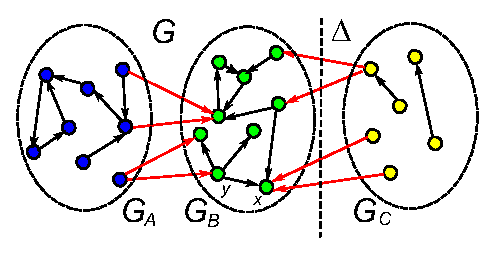
\includegraphics[scale=0.7]{fig/General_framework_peak.eps}
\vspace{-1ex}
\caption{\small An example of incremental TWPageRank computation}
\label{fig-inc-division}
\vspace{-3ex}
\end{figure}


\begin{example} \label{eg-layer-dag}
Figure~\ref{fig-inc-division} illustrates an example of incremental TWPageRank computation. Consider an update $\Delta$ on the original graph $G$.
%
It is obvious that the update $\Delta$ has no impacts on the SCCs of $G$, and $O^+$ defined earlier is a valid topological order of $G^+{'}$.
%
The original graph $G$ is then partitioned into affected and unaffected areas, and subgraphs $G_A$, $G_B$ and $G_C$ are associated with node sets $V_A$, $V_B$ and $\Delta V$, respectively. Here edge weight on $(y, x)$ changes due to the change of the peak time of node $x$, and, hence, node $y$ as well as all nodes reachable from $y$ are included in $G_B$.
%
When updating the TWPageRank scores, following $O^+$, scores of nodes in $G_C$, $G_B$ and $G_A$ are computed by iterations from scratch, by iterations with Eq.~(\ref{eq-inc-prscc}) using the existing TWPageRank vector and by scaling, respectively.
\end{example}

\vspace{-1ex}
\begin{theorem}
\label{lemma-subgraphA}
The TWPageRank vector $PR^+$ returned by~\inctwprscc converges such that $||PR^+-PR^{*}||_1 < \epsilon$, where $PR^{*}$ is the convergent TWPageRank vector.
\end{theorem}

\eat{
\begin{proofSketch}
Assume a topological order $v_1'/\dots/v_{l}'$ of the block-wise graph $G^+{'}$ where $l=|O^+|$. It suffices to prove by induction that the sum of changes of $PR^+(v)$ ($v\in scc_k$) is no more than $\epsilon |scc_k|/|V^+|$ for $scc_k$ of $v_k'$ ($k\in [1,l]$).
%The conclusion follows combining Lemma~\ref{prop-prscc}
%(see \cite{SARank-full} for details).
\end{proofSketch}
}



%Observe that (a) a topological order of the block-wise graph of $G_C$ can be computed in $O(|\Delta V|+|\Delta E|)$ time,
\markedb{Observe that (a) a topological order of the block-wise graph of $G_C$ can be computed in $O(|\Delta G|)$ time,}
(b) updating the TWPageRank scores of nodes in $V_B$ and $V_C$ costs $O(|V_B\cup V_C|+|E_{B,a}\cup E_{C,a}\cup E_{CB}|)+t^+|E_{B,i}\cup E_{C,i}|)$ time, where $t^+$ is  the maximum number of iterations among all \sccs in $G_B$ and $G_C$, and, finally, (c) updating the scores of nodes in $V_A$ costs $O(|V_A|)$ time. From these, the following holds.


\begin{prop} \label{lemma-inc-citation-comp}
Given an update $\Delta$ = $\Delta V\cup\Delta E$ of citation or venue graph $G(V,E)$, the TWPageRank vector of $G$ and the topological order of $G'$, algorithm \inctwprscc runs in $O(|V\cup \Delta V| + |E_{B,a}\cup \Delta E| + t^+|E_{B,i}\cup E_{C,i}|)$ time.
\end{prop}



%Note that the incremental algorithm reduces the complexity of updating subgraph $A$ from $O(|E^c_A|)$ to $O(|V^c_A|)$. It is more effective when only a small number of articles are updates, resulting in $|V^c_A|>>|V^c_B|+|V^c_C|$ and updating subgraph $A$ occupies most of the computation.

By Propositions~\ref{prop-converg} \& \ref{lemma-inc-topo} and Theorem \ref{lemma-subgraphA}, one can easily verify the correctness of algorithm \inctwprscc.
%
Note that  (a) algorithm \inctwprscc computes \sccs and derives the topological order based  on $\Delta$ only, instead of $G^{+}$,
(b) it skips edges in $E_A\cup E_{AB}$ when updating the scores of nodes in $V_A$ and $V_B$, and
(c) the number $t^+$ is very likely smaller than the number $t$ of \twprscc when updating scores of nodes in $V_B$.
%
All these make \inctwprscc faster than \twprscc even though they have very similar time complexity.
%, as will also been shown by the experimental study,

\eat{  %% time & space complexity
\stitle{Time \& space complexity analyses of the incremental algorithm}.
By the analyses above, the time complexity of \incensemble is the same as \batensemble, except that \incensemble saves $O(|E^c_A\cup E^c_{AB}|)$ and $O(|E^v_A\cup E^v_{AB}|)$ time on the updated citation and venue graphs. And its space complexity is also the same as \batensemble, except that it uses $(|V^c\cup \Delta V^c|+|V^v\cup\Delta V^v|)$ extra space to store the affected/unaffected areas and $(|E^c\cup \Delta E^c|+|E^v\cup \Delta E^v|)$ extra space to store the original edge weights before update.
} %% eat

\stitle{Time complexity analysis of the incremental algorithm}.
By the analyses above, the time complexity of \incensemble is the same as \batensemble, except that \incensemble saves $O(|E^c_A\cup E^c_{AB}|)$ and $O(|E^v_A\cup E^v_{AB}|)$ time when computing TWPageRank  on the updated citation and venue graphs with an extra space cost for the affected/unaffected division and the copy of original edge weights.


Despite of its similar time complexity to \batensemble, algorithm \incensemble typically achieves a substantial efficiency improvement over \batensemble, according to our statistics of affected/unaffected areas given a yearly update, \ie articles of 2011 on \aan and 2015 on \aminer and \magdata, respectively, shown in Table~II.
%
%(a) It saves $O(|V^c|+|E^c|)$ and $O(|V^v|+|E^v|)$ time when maintaining \sccs and the topological order based on the update data only,
\markedb{(a) It saves $O(|G^c|)$ and $O(|G^v|)$ time when maintaining \sccs and the topological order based on the update data only,}
%where ($|V^c|$, $|E^c|$, $|V^v|$, $|E^v|$) are more than (92\%, 89\%, 93\%, 89\%) of ($|V^{c,+}|$, $|E^{c,+}|$, $|V^{v,+}|$, $|E^{v,+}|$) on all tested graphs;
where ($|V|$, $|E|$) are more than (92\%, 89\%) of ($|V^{+}|$, $|E^{+}|$) on all tested citation and venue graphs;
(b) It saves $O(|E^c_A \cup E^c_{AB}|)$ time when updating scores on $V^c$, where edges in $E^c_A\cup E^c_{AB}$ account for more than 28\% of total;
(c) It saves $O(|E^c|)$ time when computing popularity of articles, which accounts for more than 89\% of total;
Finally, (d) it is likely to compute TWPageRank scores on $V^c_B$ and $V^v_B$ with less iterations.



%%%%%%%%%%%%%%%%%%%%%%%%%%%%%%%%%%%%%%%%%%%%%%%%%%
\begin{table}[tb!]
%\vspace{-2ex}
\begin{center}
\caption{\small Statistics of affected/unaffected areas}
\label{tab-inc}
%\begin{small}
\vspace{-.5ex}
\eat{
\begin{tabular}{|c|c|c|}
\hline
{\bf Graphs} & $|V_A|$\hspace{2ex}$|V_B|$\hspace{3ex}$|V_C|$ & $|E_A|$\hspace{2ex}$|E_{AB}|$\hspace{2ex}$|E_B|$\hspace{2ex}$|E_{CB}|$\hspace{2ex}$|E_C|$ \\
\hline \hline
% citation graphs
\aan & $46.9\%$\ $47.3\%$\ $5.8\%$ & \ $2.9\%$\ $25.9\%$\ $60.5\%$\ $10.4\%$ \hspace{1ex} $0.3\%$ \\
\aminer & $81.4\%$ \hspace{1ex} $10.7\%$ \hspace{1ex} $7.8\%$ & $18.0\%$ \hspace{1ex} $53.2\%$ \hspace{1ex} $25.1\%$ \hspace{1ex} \ $2.3\%$ \hspace{1ex} $1.4\%$ \\
\magdata & $69.5\%$ \hspace{1ex} $25.9\%$ \hspace{1ex} $4.5\%$ & \ $1.0\%$ \hspace{1ex} $27.4\%$ \hspace{1ex} $64.5\%$ \hspace{1ex} \ $7.0\%$ \hspace{1ex} $0.1\%$ \\ \hline
% venue graphs
\aan & \ $2.1\%$ \hspace{1ex} $92.0\%$ \hspace{1ex} $5.8\%$ & \ $1.0\%$ \hspace{1ex} \ $1.0\%$ \hspace{1ex} $88.8\%$ \hspace{1ex} $10.0\%$ \hspace{1ex} $0.2\%$ \\
\aminer & $45.8\%$ \hspace{1ex} $47.7\%$ \hspace{1ex} $6.4\%$ & \ $0.0\%$ \hspace{1ex} \ $3.2\%$ \hspace{1ex} $95.4\%$ \hspace{1ex} \ $1.0\%$ \hspace{1ex} $0.1\%$ \\
\magdata & $12.4\%$ \hspace{1ex} $84.6\%$ \hspace{1ex} $3.0\%$ & \ $0.0\%$ \hspace{1ex} \ $0.1\%$ \hspace{1ex} $92.6\%$ \hspace{1ex} \ $7.1\%$ \hspace{1ex} $0.1\%$ \\
 \hline
\end{tabular}
}
\begin{tabular}{|c|c c c|c c c|}
\hline
 & \multicolumn{3}{c|}{\bf Citation graphs on}   & \multicolumn{3}{c|}{\bf Venue graphs on}    \\
\raisebox{1ex}[0pt]{\bf Statis.} & \aan & \aminer & \magdata & \aan & \aminer & \magdata \\
\hline \hline
$|V_A|$ & 47.4\% & 52.3\% & 69.2\% & 2.1\% & 8.7\% & 12.4\% \\
$|V_B|$ & 46.8\% & 40.0\% & 26.3\% & 92.0\% & 84.8\% & 84.6\% \\
$|V_C|$ & \ 5.8\% & \ 7.8\% & \ 4.5\% & \ 5.8\% & \ 6.4\% & \ 3.0\% \\ \hline
$|E_A|$ & \ 3.0\% & 2.4\% & \ 0.9\% & \ 0.0\% & \ 0.0\% & \ 0.0\% \\
$|E_{AB}|$ & 26.5\% & 30.2\% & 26.6\% & \ 1.2\% & \ 0.2\% & \ 0.1\% \\
$|E_B|$ & 59.8\% & 59.3\% & 65.5\% & 88.6\% & 92.3\% & 92.6\% \\
$|E_{CB}|$ & 10.4\% & \ 7.2\% & \ 7.0\% & 10.0\% & \ 7.3\% & \ 7.1\% \\
$|E_C|$ & \ 0.3\% & \ 0.9\% & \ 0.1\% & \ 0.2\% & \ 0.2\% & \ 0.1\% \\ \hline
\end{tabular}
%\end{small}
\end{center}
\vspace{-5ex}
\end{table}
%%%%%%%%%%%%%%%%%%%




\section{Experimental Study}
\label{sec-exp}

In this section, we present an extensive experimental study of our approach \ensemblerank, compared with competitive methods.
Using three real-life scholarly datasets (\aan, \aminer and \magdata) and two sets of ground-truth (\recom and \fcita), we conducted four sets of experiments to evaluate: (1) the effectiveness of \ensemblerank,
%two sets of benchmark article pairs (\recom and \fcita) ranked by numbers of recommendations and future citations,
(2) the efficiency of our batch algorithm \batensemble and incremental algorithm \incensemble, and (3) the impacts of parameters. %\ie time decaying factor $\sigma$, importance weighting factor $\lambda$ and aggregating parameters $\alpha$ and $\beta$.

\subsection{Experimental Settings}

We first present the settings of our experimental study.

\eat{
%%%%%%%%%%%%%%%%%%%%%%%%%%%%%%%%%%%%%%%%%%%%%%%%%%
\begin{table}[t!]
%\vspace{-2ex}
\label{tab-statistics}
\begin{center}
\begin{scriptsize}
\vspace{1ex}
\begin{tabular}{|c|c|c|}
\hline
{\bf Entity / Relation}       &  {\bf Quantity in Phase~1}     & {\bf Quantity in Phase~2} \\
\hline\hline
Paper      &  $122,675,085$       &  $120,887,833$ \\ \hline
Author      &  $123,017,488$       &  $119,892,201$ \\ \hline
Venue      &  $24,841$       &  $24,843$ \\ \hline
Affiliation      &  $2,716,493$       &  $19,849$ \\ \hline
Fields of study     &  $53,834$       &  $53,830$ \\ \hline
Reference      &  $757,462,733$       &  $952,364,264$ \\ \hline
P-A      &  $324,948,062$       &  $312,034,259$ \\ \hline
P-V      &  $45,783,880$       &  $45,290,168$ \\ \hline
\end{tabular}
\vspace{-5ex}
\end{scriptsize}
\end{center}
\caption{Statistics of MAG}
\vspace{-3ex}
\end{table}
%%%%%%%%%%%%%%%%%%%
}

\stitle{Datasets}. We chose three datasets to test our approach.

\noindent
(1) \aan records the collection of computational linguistics articles published at ACL conferences from the year of 1965 to 2011~\cite{Liang16AAAI}.
It contains 18,041 articles, 14,386 authors, 273 venues and 82,944 citations.

\noindent
(2) \aminer records articles in the computer science domain from 1936 to 2016~\cite{Tang:08KDD}.
It contains 3.14 million articles, 1.74 million authors, 11,619 venues and 6.38 million citations.

\noindent
(3) \magdata records articles of various disciplines from 1800 to 2016~\cite{Sinha15:MAG}.
It contains around 127 million articles, 115 million authors, 24,024 venues and 529 million citations.
%Please refer to~\cite{Sinha15:MAG} for more details about \magdata.

To alleviate the issue of citation missing in \aminer, we added citations by title matching  based on \magdata, and the finally total number of citations is is 14.26 million. These datasets were further cleaned by deleting self-citations and citations from old articles to new ones, which accounted for (0.1\%, 0.8\%, 0.4\%) of the total citations on (\aan, \aminer, \magdata), respectively.
%from old articles to more recent ones
%These datasets were further cleaned by detecting citation cycles and removing those edges violating the temporal order if any.

%The original datasets does not strictly follow the temporal order due to the data quality problem. We hence dealt with the issuef by repeatedly detecting cycles in citation graphs and removing edges that break temporal order, if existing, or all edges in cycles.


%Actually, the citation networks of scholarly article in the three datasets are not DAG, since there are some mistaken citaions which can't be found in the references of articles. In order to delete these edges to make sure the citation network is a DAG, we do the followings:
%(1) Detect possible loops in the network by depth-first-search
%(2) Delete the edges with time error in loops found in (1) which are edges from earlier articles to later, only if all the edges in the loop haven't be deleted
%(3) Delete all the edges in loops found in (1) only if all the edges in the loop haven't be deleted
%(4) Repeat (1)-(3) until there is no loop in the network.


\stitle{Accuracy metric and ground-truth}.
We adopted the {\em pairwise accuracy} introduced by Microsoft~\cite{Richardson06:BPR,wsdmcup} to evaluate the ranking quality, \ie the fraction of times that a ranking agrees with the correct ranking orders of scholarly article pairs:


\vspace{-1ex}
\begin{small}
\begin{equation}
\label{eq-metric}
\PairAcc=\frac{\#\mbox{ of agreed pairs}}{\# \mbox{ of all pairs}}.
%\PairAcc=(\#\mbox{ of agreed pairs}) / (\# \mbox{ of all pairs}).
\end{equation}
\end{small}
\vspace{-2ex}

We constructed two sets of ground-truth importance orders of article pairs with \recom and \fcita.


\noindent
(1) \recom assumes that scholarly articles with more recommendations are of higher importance.
%
%evaluates the importance of scholarly articles by the numbers of recommendations (from textbooks and/or university course reading lists).
We used the numbers of recommendations of 93 articles on \aan~\cite{Liang16AAAI}, %which are recommended by 2 to 10 times,
and, by exact title matching, %then matched articles in \aminer and \magdata with titles.  Finally, we
generated (2133, 966, 1972) scholarly article pairs on (\aan, \aminer, \magdata), respectively.
%These articles were further matched into \aminer and \magdata through titles, which generated 966 and 1,972 article pairs for \aminer and \magdata, respectively.


\noindent
(2) \fcita assumes that scholarly articles with more citations are of higher importance.
%
However, the number of entire citations is obviously biased to old articles. Some work adopts the number of future citations~\cite{Wang13AAAI,Wang16TIST,Li08TSRanking}, which is also not appropriate since this only estimates of future impacts of articles, not at the concerned time. For a fair ranking benchmark, we propose to use both past and future citations with the same period of time \wrt\ the concerned time, such that the number of citations within these two periods reveals the importance of articles at the concerned time.
%
We hence divided each dataset into two parts with a splitting (concerned) time such that (a) the data before the splitting time is used for ranking model, (b) the remain part of data is used to collect future citations, and (c) the most recent part of the data for ranking model with the same time span as the future citations is used to collect past citations.
%
%
Moreover, articles in the same pair were required to be in similar research fields, by utilizing the Fields-Of-Study information on \magdata~\cite{Sinha15:MAG}, and published in the same year, similar to~\cite{Wang16TIST}.
We used all pairs (around 50,000) for \aan, and randomly chose 300,000 pairs for both \aminer and \magdata.

\eat{
\noindent
(2) \fcita assumes that scholarly articles with more future citations are of higher importance~\cite{Wang13AAAI,Wang16TIST,Li08TSRanking}.
We first divided each dataset into ranking part and evaluation part by a splitting year such that data before the splitting year were used for ranking and the remaining data were used to count the numbers of future citations for articles in the ranking part.
%
Moreover, articles in the same pair were required to be in similar research fields, by utilizing the Fields-Of-Study information on \magdata~\cite{Sinha15:MAG}, and published in the same year, similar to~\cite{Wang16TIST}.
We used all pairs (around 25,000) for \aan, and randomly chose 300,000 pairs for both \aminer and \magdata.
%
\marked{Due to the sparse citations on \aminer, the two articles in 50\% pairs have 0 and 1 future citation, which is a very weak evidence for importance order. Hence, we further required articles in pairs must have at least 1 future citation on \aminer.}
%Finally, we generated  26,987 article pairs for \aan, and randomly selected 300,000 article pairs for both \aminer and \magdata.
}%% eat


\stitle{Algorithms}.
We compared our approach with three competitive methods: \pagerank~\cite{Brin98:PageRank}, \futurerank~\cite{sayyadi09} and \hhgrank~\cite{Liang16AAAI}.

\noindent
(1) \pagerank (PageRank) is a classic method that uses only citation information to rank scholarly articles.
%and articles are ranked according to PageRank scores computed on the citation graph.


\noindent
(2) \futurerank (FutureRank) combines citation, temporal and other heterogeneous information to rank scholarly articles.
%by predicting their future PageRank.
%is a \pagerank based ranking methods which is able to evaluate the importance of articles by predicting their future ranking. In order to do that, it uses both citation network and other available information such as the authorship network and the publication time of the articles.

\noindent
(3) \hhgrank (HHGBiRank) is a very recent method using both citation and heterogeneous information, such that heterogeneous entities are mutually reinforced based on hypernetworks.
%It uses hypernetworks to propagate importance/authority between entities.
%a scientific literature ranking algorithm based on the heterogeneous academic hypernetwork. An ingredient of \hhgrank is based on the fact that, the importance of scholarly articles not only depends on the frequency it has been cited and the quality of citation but also depends on the importance of authors and researchers of the paper.


\stitle{Implementation}.
All algorithms were implemented with Microsoft Visual C++.
%Parameters.
For all algorithms, (a) the damping parameter $d$ and the iteration threshold $\epsilon$ were fixed to 0.85 and $10^{-8}$, respectively,
(b) the default splitting years were selected such that the part of data for ranking model accounted for around 75\% of the entire data, which were 2008 on \aan and 2012 on both \aminer and \magdata, and,
(c) for the sake of fairness, aggregating parameters of \futurerank, \hhgrank and \ensemblerank were tuned at the granularity of 0.1 and the best results were reported.
%
Moreover, $\rho$ was set to -0.2 for \futurerank following~\cite{sayyadi09}, and the time decaying factor $\sigma$ and the importance weighting factor $\lambda$ were set to -1 and 0.5  by default for \ensemblerank.

All experiments were conducted on a PC with 2 Intel Xeon E5--2630 2.4GHz CPUs and 64 GB of memory, running 64 bit Windows 7 professional system. The usage of virtual memory was forbidden. %in all of our tests.
When quantity measures are evaluated, the test was repeated over 5 times and the average results are reported.

%%%%%%%%%%%%%%%%%%%%%%%%%%%%%%%%%%%%%%%%%%%%%%%%%%
\begin{table}[t!]
%\vspace{-2ex}
\label{tab-result}
\begin{center}
\caption{\small Accuracy tests with \recom}
%\begin{small}
%\vspace{-.5ex}
\begin{tabular}{|c|c|c|c|c|}
\hline
{\bf Datasets}   &  \hspace{1ex}\pagerank\hspace{1ex}     & \hspace{1ex}\futurerank\hspace{1ex}  &  \hspace{1ex}\hhgrank\hspace{1ex}  &   \hspace{1ex}\ensemblerank\hspace{1ex}    \\
\hline \hline
\aan  & $0.671$   & $0.738$   & $0.758$     & {\bf 0.805}      \\  %\hline
\aminer  & $0.651$   & $0.729$   & $0.730$     & {\bf 0.778}      \\ %\hline
\magdata  & $0.615$   & $0.655$   & $0.658$     & {\bf 0.680}      \\ \hline
\end{tabular}
%\vspace{-.5ex}
%\end{small}
\end{center}
\vspace{-4ex}
\end{table}
%%%%%%%%%%%%%%%%%%%




\newcommand{\graphscale}{0.36} %0.38
\newcommand{\graphmargin}{-4ex}
\newcommand{\exppath}{./exp/}
%\newcommand{\exppath}{./exp/wpr/}
%%% all in 1 Figure
\begin{figure*}[tb!]
%\vspace{-2ex}
\addtolength{\subfigcapskip}{-1ex}
\begin{center}
%\hspace{10ex}
\subfigure[{\scriptsize \aan}]{\label{exp-aan-futureyear}
\includegraphics[scale=\graphscale]{\exppath AAN_PairAcc1.eps}}
%\quad\quad
\hspace{\graphmargin}
\subfigure[{\scriptsize \aan}]{\label{exp-aan-t}
\includegraphics[scale=\graphscale]{\exppath AAN_PairAcc2.eps}}
%\quad\quad
\hspace{\graphmargin}
\subfigure[{\scriptsize \aan}]{\label{exp-aan-fcdiff}
\includegraphics[scale=\graphscale]{\exppath AAN_PairAcc3.eps}}
%\quad\quad
\hspace{\graphmargin}
\subfigure[{\scriptsize \aan}]{\label{exp-aan-sigma}
\includegraphics[scale=\graphscale]{./exp/AAN_sigma2.eps}}
%\quad\quad
\hspace{\graphmargin}
\subfigure[{\scriptsize \aan}]{\label{exp-aan-lambda}
\includegraphics[scale=\graphscale]{./exp/AAN_lambda.eps}}
\\ %%%%%%%%%%%%%%%%%%%%%%%%%%%%%%%%%%%%%%
\vspace{-1.5ex}
\subfigure[{\scriptsize \aminer}]{\label{exp-aminer-futureyear}
\includegraphics[scale=\graphscale]{\exppath AMiner_PairAcc1.eps}}
%\quad\quad
\hspace{\graphmargin}
\subfigure[{\scriptsize \aminer}]{\label{exp-aminer-t}
\includegraphics[scale=\graphscale]{\exppath AMiner_PairAcc2.eps}}
%\quad\quad
\hspace{\graphmargin}
\subfigure[{\scriptsize \aminer}]{\label{exp-aminer-fcdiff}
\includegraphics[scale=\graphscale]{\exppath AMiner_PairAcc3.eps}}
%\quad\quad
\hspace{\graphmargin}
\subfigure[{\scriptsize \aminer}]{\label{exp-aminer-sigma}
\includegraphics[scale=\graphscale]{./exp/AMiner_sigma2.eps}}
%\quad\quad
\hspace{\graphmargin}
\subfigure[{\scriptsize \aminer}]{\label{exp-aminer-lambda}
\includegraphics[scale=\graphscale]{./exp/AMiner_lambda.eps}}
\\%%%%%%%%%%%%%%%%%%%%%%%%%%%%%%%%%%%%%%%%%%%
\vspace{-1.5ex}
\subfigure[{\scriptsize \magdata}]{\label{exp-mag-futureyear}
\includegraphics[scale=\graphscale]{\exppath MAG_PairAcc1.eps}}
%\quad\quad
\hspace{\graphmargin}
\subfigure[{\scriptsize \magdata}]{\label{exp-mag-t}
\includegraphics[scale=\graphscale]{\exppath MAG_PairAcc2.eps}}
%\quad\quad
\hspace{\graphmargin}
\subfigure[{\scriptsize \magdata}]{\label{exp-mag-fcdiff}
\includegraphics[scale=\graphscale]{\exppath MAG_PairAcc3.eps}}
%\quad\quad
\hspace{\graphmargin}
\subfigure[{\scriptsize \magdata}]{\label{exp-mag-sigma}
\includegraphics[scale=\graphscale]{./exp/MAG_sigma2.eps}}
%\quad\quad
\hspace{\graphmargin}
\subfigure[{\scriptsize \magdata}]{\label{exp-mag-lambda}
\includegraphics[scale=\graphscale]{./exp/MAG_lambda.eps}}
\end{center}
\vspace{-1.5ex}
\caption{\small Accuracy tests with \fcita (all) and \recom ((d)--(e), (i)--(j) and (n)--(o))}
\label{exp-pairacc}
\vspace{-1ex}
\end{figure*}
%%%%%%%%%%%%%%%%%%%%%%%%%%%%%%%%%%%%%%
\begin{figure*}[tb!]
%\vspace{1ex}
\addtolength{\subfigcapskip}{-1ex}
\begin{center}
%\hspace{10ex}
\subfigure[{\scriptsize TWPageRank (batch vs. inc.)}]{\label{exp-aminer-time1}
\includegraphics[scale=\graphscale]{./exp/AMiner_time_twpr.eps}}
\hspace{0ex}
%\hfill
\subfigure[{\scriptsize Comparison of ranking algorithms}]{\label{exp-aminer-time2}
\includegraphics[scale=\graphscale]{./exp/AMiner_time.eps}}
\hspace{0ex}
%\hfill
\subfigure[{\scriptsize TWPageRank (batch vs. inc.)}]{\label{exp-mag-time1}
\includegraphics[scale=\graphscale]{./exp/MAG_time_twpr.eps}}
\hspace{0ex}
%\hfill
\subfigure[{\scriptsize Comparison of ranking algorithms}]{\label{exp-mag-time2}
\includegraphics[scale=\graphscale]{./exp/MAG_time.eps}}
\end{center}
\vspace{-1.5ex}
\caption{\small Efficiency tests on \aminer ((a)--(b)) and  \magdata ((c)--(d))}
\label{exp-time}
\vspace{-2ex}
\end{figure*}
%%%%%%%%%%%%%%%%%%%%%%%%%%%%%%%%%%

\subsection{Experimental Results}
\label{subsec-expres}

We next present our findings.

\stitle{Exp-1: Effectiveness with \recom}.
%\subsubsection{Exp-1: Effectiveness with \recom}
In the first set of our tests, we used ground-truth \recom to evaluate the effectiveness of our approach.
All algorithms used articles published before 2012, since article pairs of \recom were from this portion of articles.
Aggregating parameters were selected as follows: $(\alpha,\beta,\gamma)$ = $(0.1, 0.2, 0.2)$ for \futurerank, $(a_{i1},a_{i2},a_{i3})$ = $(0.6, 0.2, 0.2)$ for \hhgrank ($i\in[1,3]$), and $(\alpha,\beta)$ = $(0.1, 0.8)$ for \ensemblerank.
%The venue ensemble contributed most in \ensemblerank, indicating that venue information plays a key role when people recommend scholarly articles.
The results of \PairAcc are reported in Table~III.

The \PairAcc of \pagerank is much lower than the one of other algorithms, indicating that citation information alone is insufficient for scholarly article ranking, and other information helps to refine the results. Moreover, \ensemblerank consistently ranks better than all competitors. Indeed, \ensemblerank improves the \PairAcc over (\pagerank, \futurerank, \hhgrank) by (13.5\%, 6.8\%, 4.8\%) on \aan, (12.7\%, 5.0\%, 4.9\%) on \aminer, and (6.5\%, 2.5\%, 2.2\%) on \magdata, respectively.

\stitle{Exp-2: Effectiveness with \fcita}.
%\subsubsection{Exp-2: Effectiveness with \fcita}
In the second set of tests, we used ground-truth \fcita to evaluate the effectiveness.
%All algorithms produced results based on articles in ranking data.
Aggregating parameters were selected as follows: $(\alpha, \beta, \gamma)$ = $(0.7, 0.1,$ $0.2)$ for \futurerank, $(a_{i1}, a_{i2}, a_{i3})$ = $(0.3, 0.6, 0.1)$ for \hhgrank ($i\in[1, 3]$), and $(\alpha, \beta)$ = $(0.8, 0.1)$ for \ensemblerank.
%Here the citation component contributed most in \ensemblerank, since \fcita is based on citation information.
To evaluate the effectiveness of ranking in different scenarios, we varied three factors in our tests: the splitting year $Y_s$, the number $T_p$ of published years of articles, and the difference $dif$ of future citation counts.
%
Given $Y_s$, $T_p$ and $dif$, we only used article pairs whose articles were published within $[Y_s - T_p, Y_s)$ and the difference of future citation counts was equal to or larger than $dif$ to test the \PairAcc.
% no earlier than $T_p$ years before $Y_s$



%varying number of years as future period
\etitle{Exp-2.1}.
%\stitle{Exp-2.1}.
To evaluate the effectiveness of ranking \wrt\ {\em short-term and long-term importance},
we varied the splitting year $Y_s$ from 2006 to 2011 on \aan and from 2010 to 2015 on both \aminer and \magdata, while fixed $T_p$ = $+\infty$ and $dif$ = $1$, \ie using all scholarly article pairs.
%
Intuitively, large and small $Y_s$ correspond to short-term and long-term importance, respectively.
The results of \PairAcc are reported in Figs.~\ref{exp-aan-futureyear}, \ref{exp-aminer-futureyear} and \ref{exp-mag-futureyear}, in which the red markers $\Box$ in dashed lines mean that \hhgrank ran out of memory.

%For each $Y_s$ we generated benchmark pairs as described earlier, and tested \PairAcc using all pairs, \ie $b$ = $+\infty$, $dif$ = $1$.
%We did not use the latest year since the complete articles have not been included yet.

When varying $Y_s$, the \PairAcc of all algorithms increases with the increment of $Y_s$ on both \aminer and \magdata, indicating that it is easier to assess short-term (large $Y_s$) than long-term (small $Y_s$) importance. While the results on \aan do not follow this trend, possibly because \aan does not record the complete articles of 2007 and 2009.
Moreover, \ensemblerank consistently ranks better than all competitors, regardless of assessing short-term or long-term importance.
Indeed, \ensemblerank improves the \PairAcc over (\pagerank, \futurerank, \hhgrank) by (17.9\%, 5.4\%, 5.5\%) on \aan, (18.6\%, 7.7\%, 5.8\%) on \aminer, and  (16.7\%, 7.2\%, 2.9\%) on \magdata, respectively.



%varying number of years as evaluate period.
\etitle{Exp-2.2}.
%\stitle{Exp-2.2}.
To evaluate the effectiveness of ranking \wrt\ {\em the published time of articles},
we varied the number $T_p$ of published years from 1 to $+\infty$, while fixed $Y_s$ to default values of three datasets and $dif=1$, respectively. The results of \PairAcc are reported in Figs.~\ref{exp-aan-t}, \ref{exp-aminer-t} and \ref{exp-mag-t}.


When varying $T_p$, the \PairAcc of all algorithms increases with the increment of $T_p$, since old articles (large $T_p$) are easier to rank based on adequate information, while new articles (small $T_p$) are hard to rank with little information available. Moreover, \ensemblerank consistently ranks better than all competitors, especially when $T_p\le3$, \ie ranking recently published articles. Indeed, \ensemblerank improves the \PairAcc over (\pagerank, \futurerank, \hhgrank) by (19.0\%, 3.1\%, 3.9\%) on \aan, (25.0\%, 8.2\%, 6.3\%) on \aminer, and (23.6\%, 8.3\%, 3.2\%) on \magdata, on average, respectively.


%varying difference of future citation count in benchmark
\etitle{Exp-2.3}.
%\stitle{Exp-2.3}.
To evaluate the effectiveness of ranking \wrt\ {\em the difference of future citations},
we varied the difference $dif$ of future citation counts from 1 to 7, while fixed $Y_s$ to default values of three datasets and $T_i=+\infty$. The results of \PairAcc are reported in Figs.~\ref{exp-aan-fcdiff}, \ref{exp-aminer-fcdiff} and \ref{exp-mag-fcdiff}.

When varying $dif$, the \PairAcc of all algorithms increases with the increment of $dif$, since scholarly article pairs with larger $dif$ are easier to rank. Moreover, \ensemblerank consistently ranks better than all competitors, regardless of easy or difficult article pairs. Indeed, \ensemblerank improves the \PairAcc over (\pagerank, \futurerank, \hhgrank) by (12.0\%, 3.0\%, 3.2\%) on \aan, (14.0\%, 6.5\%, 4.6\%) on \aminer, and (13.4\%, 6.0\%, 2.4\%) on \magdata, on average, respectively.

%The pair accuracy results tell us that (a) \ensemblerank outperforms other methods on all datasets with all difference of future citation count and obtains the highest accuracy when the difference is greater than 6, and (b) the accuracy of all method increases with the addition of difference of future citation count which means it is easier for all methods to evaluate the importance of two scholarly articles in one pair when there is a obvious different between them. Our algorithm \ensemblerank improves the pair accuracy over \pagerank, \futurerank and \hhgrank by $(15.7\%, 2.8\%, 3.9\%)$ on \aan, $(17.3\%, 7.6\%, 5.8\%)$ on \aminer, and $(10.3\%, 4.4\%, 1.6\%)$ on \magdata, when evaluate all the pairs which have difference of future citation count greater than 0, which means \ensemblerank can evaluate and distinguish the articles only have small difference better.


\stitle{Exp-3: Efficiency}.
%\subsubsection{Exp-3: Efficiency}
In the third set of tests, we evaluated the efficiency of our algorithms.
%
We compared our algorithms with \powtwprscc and \powensemble, which were the same to \twprscc and \batensemble except using power method for TWPageRank computation, and with algorithms \futurerank and \hhgrank.
Here \pagerank was omitted due to its effectiveness.
%
We varied the splitting year $Y_s$ from 2009 to 2016 and tested the running time on both \aminer and \magdata.
%
For incremental algorithms, base and update parts consisted of data before 2008 and within $[2008, Y_s)$, respectively.
%And the incremental ratio evaluated by the size of data was 0.11, 0.25, 0.39, 0.55, 0.73, 0.93, 1.14 and 1.30 for $Y_s\in[2009,2016]$.
%
The results of running time are reported in Fig.~\ref{exp-time}, where the red markers $\Box$ in dashed lines mean that \hhgrank ran out of memory.
%The results on the large data \magdata are reported in Fig.~\ref{exp-time}, where red markers \marked{$\Box$} in dashed line mean \hhgrank ran out of memory, and the results on \aminer are left in~\cite{SARank-full}.

When varying $Y_s$, the running time of all algorithms increases with the increment of $Y_s$, and our incremental algorithms
consistently run faster than all competitors, especially with less update data.
%
For TWPageRank computation, algorithm \inctwprscc is on average (1.9, 3.8) and (2.5, 4.1) times faster than (\twprscc, \powtwprscc) on \aminer and \magdata, respectively.
%
For scholarly article ranking, algorithm \incensemble is on average (1.7, 3.1, 2.8, 117) and (2.0, 3.0, 4.4, 245) times faster than (\batensemble, \powensemble, \futurerank, \hhgrank) on \aminer and \magdata, respectively.

%\etitle{Remarks}.
In our tests we adopted a yearly update policy due the limitation of  available time information. In practice our algorithms may bring more efficiency benefits since the ranking is usually more frequent, such that the data updates are smaller and the unaffected area is very likely much larger.

%algorithm \batensemble is on average (1.3, 2.5, 348) times faster than (\powensemble, \futurerank, \hhgrank), respectively. And algorithm \incensemble further improves the efficiency by 22\% on average, compared with \batensemble.


%%%%%%%%%%%%%%%%%%%%%%%%%%%%%%%%%%%%%
\newcommand{\graphscaleexpapp}{0.25}
\newcommand{\graphmarginexpapp}{-2ex}
%%% all in 1 Figure
\begin{figure*}[tb!]
\addtolength{\subfigcapskip}{-1ex}
\begin{center}
\subfigure[{\scriptsize \aan with \recom}]{\label{exp-aan-ab-recom}
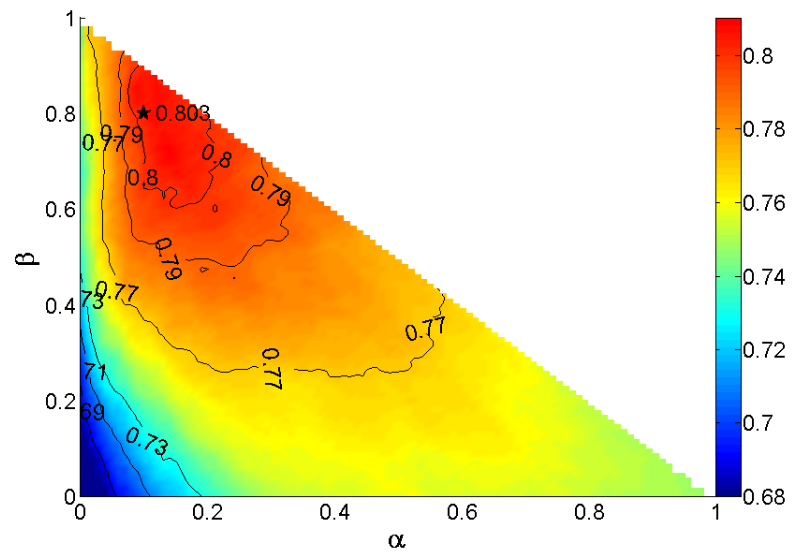
\includegraphics[scale=\graphscaleexpapp]{./exp/AAN-para-recm.eps}}
%\quad\quad
%\hspace{\graphmarginexpapp}
\hfill
\subfigure[{\scriptsize \aminer with \recom}]{\label{exp-aminer-ab-recom}
\includegraphics[scale=\graphscaleexpapp]{./exp/AMiner-para-recm.eps}}
%\quad\quad
%\hspace{\graphmarginexpapp}
\hfill
\subfigure[{\scriptsize \magdata with \recom}]{\label{exp-mag-ab-recom}
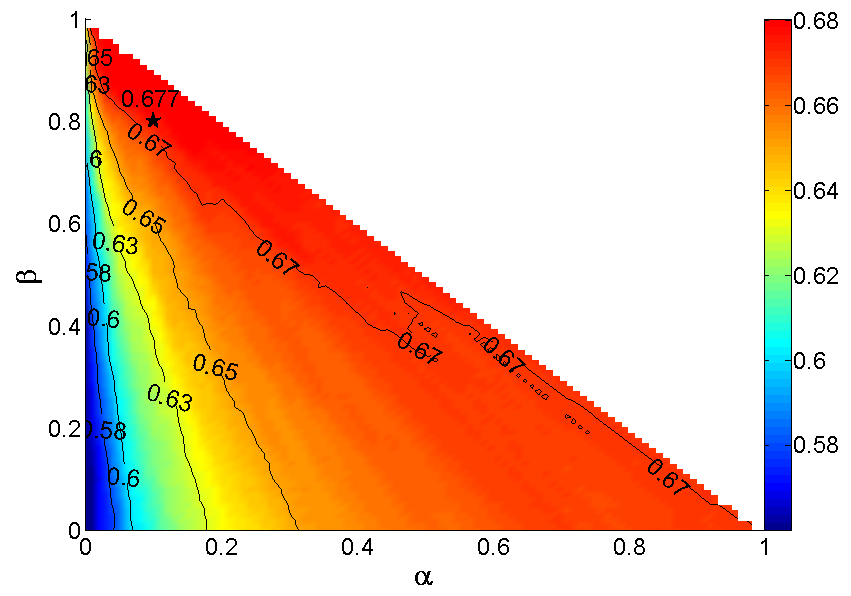
\includegraphics[scale=\graphscaleexpapp]{./exp/MAG-para-recm.eps}}
\\ %%%%%%%%%%%%%%%%%%%%%%%%%%%%%%%%%%%%%%
\vspace{-2ex}
%\hspace{-10ex}
\subfigure[{\scriptsize \aan  with \fcita}]{\label{exp-aan-ab-fcita}
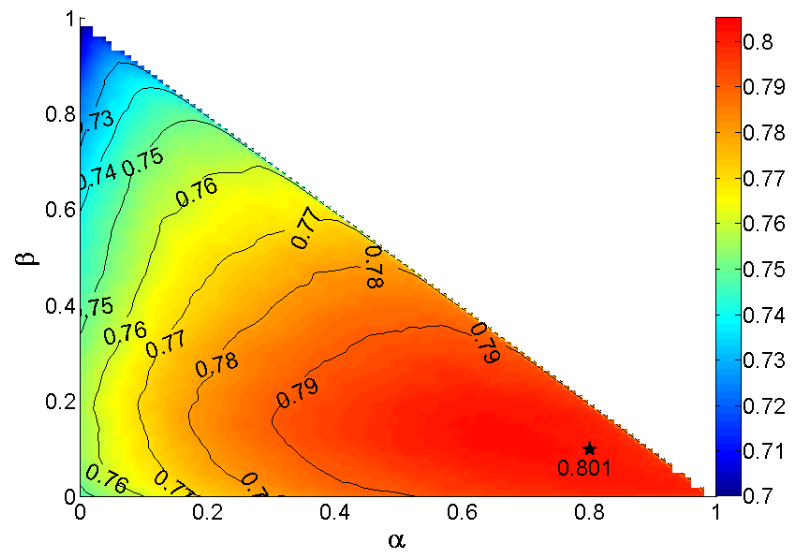
\includegraphics[scale=\graphscaleexpapp]{./exp/AAN-para-fcita.eps}}
%\quad\quad
%\hspace{\graphmarginexpapp}
\hfill
\subfigure[{\scriptsize \aminer with \fcita}]{\label{exp-aminer-ab-fcita}
\includegraphics[scale=\graphscaleexpapp]{./exp/AMiner-para-fcita.eps}}
%\quad\quad
%\hspace{\graphmarginexpapp}
\hfill
\subfigure[{\scriptsize \magdata with \fcita}]{\label{exp-mag-ab-fcita}
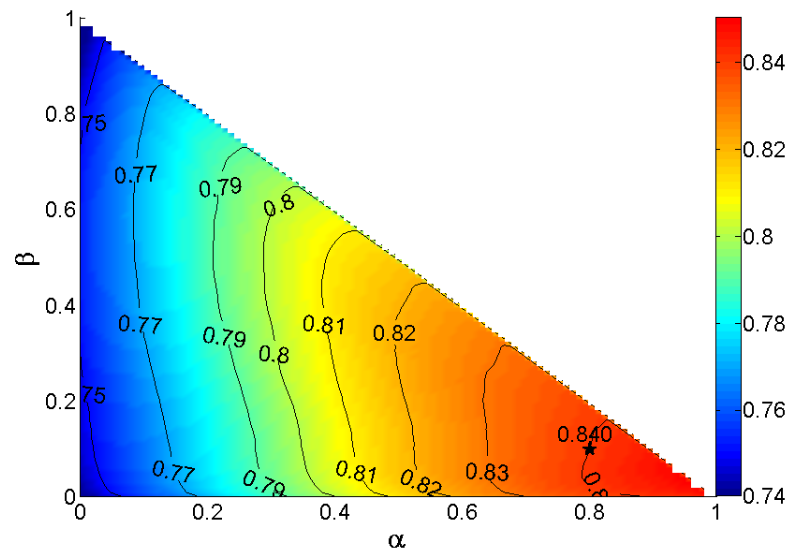
\includegraphics[scale=\graphscaleexpapp]{./exp/MAG-para-fcita.eps}}
\end{center}
\vspace{-1.5ex}
\caption{\small Accuracy tests: varying aggregating parameters $\alpha$ and $\beta$}
\label{exp-ab}
\vspace{-2ex}
\end{figure*}
%%%%%%%%%%%%%%%%%%%%%%%%%%%%%%%%%%%%%%

\stitle{Exp-4: Impacts of parameters}.
%\subsubsection{Exp-4: Impacts of parameters}.
In the last set of tests, we evaluated the impacts of time decaying factor $\sigma$, importance weighting factor $\lambda$, aggregating parameters $\alpha$ and $\beta$, and the TWPageRank. We fixed these parameters as well as $Y_s$ to their default values, used the TWPageRank proposed in this work by default, and tested the \PairAcc with the entire \recom and \fcita (\ie $T_i=+\infty$, $dif=1$).

%We present main results only and more details are available in~\cite{SARank-full}.




\etitle{Exp-4.1}.
%\stitle{Exp-4.1}.
To evaluate the impacts of the time decaying factor $\sigma$, we varied $\sigma$ from -1.6 to -0.4.
%, while fixed $Y_s$ to default values, $T_i=+\infty$, $dif=1$ and $\lambda=0.5$.
The results of \PairAcc are reported in Figs.~\ref{exp-aan-sigma}, \ref{exp-aminer-sigma} and \ref{exp-mag-sigma}.
%with both sets of ground-truth


When varying $\sigma$, the \PairAcc of \ensemblerank is very stable on all datasets using both \recom and \fcita. Indeed, with \recom and \fcita, the \PairAcc only varies (0.42\%, 1.55\%, 0.81\%) and (1.26\%, 0.96\%, 1.16\%) on (\aan, \aminer, \magdata), respectively.
%
%We omitted the detailed results of running time due to space constraint.
The running time varies (11.3\%, 8.6\%) on average only on (\aminer, \magdata), respectively.
%(0.18, 33.6) seconds, \ie

%Both of these show the robustness of \ensemblerank to the time decaying factor $\sigma$.

%As we can see from the figure, our method \ensemblerank is almost stable with the reduction of $\sigma$, since there is only a small fluctuation and the accuracy of our methods is always higher than the best baseline result in all datasets regardless of the change of $\sigma$. This means \ensemblerank is insensitive with $\sigma$.


%%%%%%%%%%%%%%%%%%%%%%%%%%%%%%%%%%%%%%%%%%%%%%%%%%
\begin{table}[tb!]
%\vspace{-2ex}
\begin{center}
\caption{\small Accuracy tests using different components with \recom (rows 2--4) and \fcita (rows 5--7).}
\label{tab-recom}
%\begin{small}
%\vspace{-.5ex}
\begin{tabular}{|c| c |c | c|}
\hline
{\bf Datasets} & {\bf C}\hspace{5ex}{\bf V}\hspace{5ex}{\bf A} & {\bf CV}\hspace{3ex}{\bf CA}\hspace{3ex}{\bf VA} & {\bf CVA} \\
\hline \hline
% \recom
\aan & 0.752 \ 0.616 \ 0.649 & 0.809 \ 0.764 \ 0.747 & {\bf 0.810} \\
\aminer & 0.735 \  0.581 \  0.640 & 0.784 \ 0.749 \ 0.729 & {\bf 0.785} \\
\magdata & 0.635 \ 0.534 \ 0.553 & 0.697 \ 0.673 \  0.648 & {\bf 0.698} \\ \hline
% \ficta
\aan & 0.785 \ 0.557 \ 0.761 & 0.849 \ 0.866 \ 0.771 & {\bf 0.870} \\
\aminer & 0.713 \  0.603 \  0.725 & 0.843 \ 0.847 \ 0.740 & {\bf 0.856} \\
\magdata & 0.736 \ 0.628 \ 0.718 & 0.848 \ 0.857 \ 0.751 & {\bf 0.874} \\
\hline
\end{tabular}
%\end{small}
\end{center}
\vspace{-4ex}
\end{table}
%%%%%%%%%%%%%%%%%%%


\etitle{Exp-4.2}.
%\stitle{Exp-4.2}.
To evaluate the impacts of importance weighting factor $\lambda$, we varied $\lambda$ from 0 to 1.
%while fixed $Y_s$ to default values, $T_i=+\infty$, $dif=1$ and $\sigma=-1.0$.
The results of \PairAcc are reported in Figs.~\ref{exp-aan-lambda}, \ref{exp-aminer-lambda} and \ref{exp-mag-lambda}. Note that parameter $\lambda$ has no impacts on efficiency.
%with both sets of ground-truth

When varying $\lambda$, the \PairAcc of \ensemblerank first increases and then decreases on all datasets with both \fcita and \recom, except on \aminer with \recom.
%\marked{The value of $\lambda$ for \ensemblerank to achieve the best effectiveness is (0.6, 0, 0.2) and (0.6, 0.4, 0.1) on (\aan, \aminer, \magdata) with \recom and \fcita, respectively.}
This result indicates that combining prestige and popularity generally produces more robust results than using either of prestige and popularity.
Indeed, with \recom and \fcita, the \PairAcc of combining prestige and popularity is (10.2\%, 10.7\%, 5.5\%) and (8.0\%, 8.7\%, 9.0\%) higher than using prestige alone, and is (1.2\%, -0.1\%, 1.0\%) and (1.0\%, 1.0\%, 0.3\%) higher than using popularity alone on (\aan, \aminer, \magdata), respectively.


%The selection of $\lambda$ is influenced by ground-truth, such that the best $\lambda$ falls into $[xx,xx]$ and $[yy,yy]$ on \fcita and \recom, respectively. Moreover, equally weighting, \ie $\lambda=0.5$, is a good default setting when no query information is available in advance.
%Indeed, the best obtained \PairAcc using (\fcita, \recom) is only (0.10\%, 0.38\%), (0.04\%, 2.59\%) and (0.06\%, 0.91\%)  higher than the \PairAcc of equally weighting on \aan, \aminer and \magdata, respectively.





\etitle{Exp-4.3}.
To evaluate the impacts of aggregating parameters $\alpha$ and $\beta$, we varied $\alpha$ and $\beta$ at the granularity of 0.01. Again, parameters $\alpha$ and $\beta$ have few impacts on efficiency. The results are reported in Fig.~\ref{exp-ab}, where the parameters selected earlier and their corresponding \PairAcc are marked with $*$.

When varying $\alpha$ and $\beta$, the \PairAcc of \ensemblerank changes gently, as shown in Fig.~\ref{exp-ab}.
The optimal \PairAcc is obtained within a single region, rather than a complex collection of optimal regions.
%
Moreover, the \PairAcc keeps at a high level within a certain ($\alpha$, $\beta$) combination space around the optimal region, as shown in Fig.~\ref{exp-ab}.
%For instance, consider a square of length 0.3, which covers 8.5\% of the parameter combination space. The fraction of parameters such that the \PairAcc is no worse than 1\% of the corresponding \PairAcc with marker $*$ is (73\%, 94\%) on \aan, (96\%, 87\%) on \aminer and (83\%, 95\%) on \magdata, using (\recom, \fcita), respectively.
%
Further, the optimal parameters on the same sets of ground-truth are very similar for (\aan, \aminer and \magdata), indicating that the setting of $\alpha$ and $\beta$ can be easily transferred across different datasets.
To conclude, \ensemblerank is very robust to parameters $\alpha$ and $\beta$, and it is quite flexible for choosing proper values of parameters $\alpha$ and $\beta$.

Moreover, this enables to verify the effectiveness of importance assembling from different components, whose results are reported in Table~IV, in which letters C, V and A stand for citation, venue and author components, respectively.
The ranking based on all components consistently performs the best, using both \recom and \fcita, which justifies the use of importance assembling for ranking scholarly articles.
%which, using \recom and \fcita, improves the \PairAcc over using components (C, V, A, CV, CA, VA) by (5.77\%, 19.4\%, 16.1\%, 0.09\%, 4.59\%, 6.28\%) and (9.54\%, 23.7\%, 5.90\%, 2.50\%, 0.71\%, 4.79\%) on \aan, (6.94\%, 23.7\%, 14.4\%, 0.21\%, 1.56\%, 7.67\%) and (17.68\%, 12.4\%, 9.61\%, 0.33\%, 1.88\%, 6.34\%) on \aminer, and (6.29\%, 16.38\%, 14.45\%, 0.05\%, 2.43\%, 5.02\%) and (11.43\%, 19.2\%, 11.2\%, 1.44\%, 0.77\%, 9.62\%) on \magdata, respectively.


\eat{
\etitle{Exp-4.3}.
%\stitle{Exp-4.3}.
To evaluate the impacts of aggregating parameters $\alpha$ and $\beta$, we varied $\alpha$ and $\beta$ at the granularity of 0.01.
%while fixed $Y_s$ to default values, $T_i=+\infty$, $dif=1$, $\sigma=-1.0$ and $\lambda=0.5$.
Again, parameters $\alpha$ and $\beta$ have few impacts on efficiency. Due to space limitations, we only present the main results and more details are available at~\cite{SARank-full}.

Indeed, \ensemblerank is very robust to parameters $\alpha$ and $\beta$.
(a) When varying $\alpha$ and $\beta$, the \PairAcc of \ensemblerank changes gently. (b) \PairAcc also keeps at a high level within a certain ($\alpha$, $\beta$)  combination space. Finally, (c) the optimal parameters on the same set of ground-truth are very similar for \aan, \aminer and \magdata. That is, it is quite flexible for choosing proper values
of  parameters $\alpha$ and $\beta$.
} %%%%%%%% brief version of Exp-4.3

%%%%%%%%%%%%%%%%%%%%%%%%%%%%%%%%%%%%%%
\begin{figure*}[tb!]
%\vspace{1ex}
\addtolength{\subfigcapskip}{-1ex}
\begin{center}
\subfigure[{\scriptsize \aan with \recom}]{\label{exp-aan-recom-drank}
\includegraphics[scale=0.36]{./exp/AAN_TWPageRank_recom.eps}}
\hfill
%\hspace{\graphmarginexpapp}
\subfigure[{\scriptsize \aminer with \recom}]{\label{exp-aminer-recom-drank}
\includegraphics[scale=0.36]{./exp/AMiner_TWPageRank_recom.eps}}
\hfill
%\hspace{\graphmarginexpapp}
\subfigure[{\scriptsize \magdata with \recom}]{\label{exp-mag-recom-drank}
\includegraphics[scale=0.36]{./exp/MAG_TWPageRank_recom.eps}}
\\%%%%%%%%%%%%%%%%%%%%%%%%%%%%%%%%%%%%%%%%%%%
\vspace{-.5ex}
\subfigure[{\scriptsize \aan with \fcita}]{\label{exp-aan-fcita-drank}
\includegraphics[scale=0.36]{./exp/AAN_TWPageRank_fcita.eps}}
\hfill
%\hspace{\graphmarginexpapp}
\subfigure[{\scriptsize \aminer with \fcita}]{\label{exp-aminer-fcita-drank}
\includegraphics[scale=0.36]{./exp/AMiner_TWPageRank_fcita.eps}}
\hfill
%\hspace{\graphmarginexpapp}
\subfigure[{\scriptsize \magdata with \fcita}]{\label{exp-mag-fcita-drank}
\includegraphics[scale=0.36]{./exp/MAG_TWPageRank_fcita.eps}}
\end{center}
\vspace{-1.5ex}
\caption{\small Impacts of the TWPageRank on accuracy: varying importance weighting
factor $\lambda$}
\label{exp-drank}
\vspace{-2ex}
\end{figure*}
%%%%%%%%%%%%%%%%%%%%%%%%%%%%%%%%%%

\newcommand{\drank}{\kw{DRank}}


\etitle{Exp-4.4}.
To evaluate the impacts of our TWPageRank, we compared our \ensemblerank with \drank, an alternative of \ensemblerank by removing the peak time in  Eq.~(\ref{eq-infl-weights}) of  TWPageRank, \ie $w(u,v)=e^{\sigma(T_u-T_v)}$. % with a directly exponentially decayed impact weights without peak times, \ie , .
%The two algorithms produce the same popularity while different prestige.
To better understand the impacts, we varied the importance weighting factor $\lambda$ from 0.1 to 1. Note that the ranking results are the same when $\lambda=0$ due to the same popularity computation. The results are reported in Fig.~\ref{exp-drank}, where the numbers represent the improvement of \PairAcc by \ensemblerank over the one by \drank.


When varying $\lambda$, the \PairAcc of \ensemblerank is better than the one of \drank in most cases, which shows the superiority of the TWPageRank than exploiting exponentially decayed weights directly without introducing the peak time.
The \PairAcc difference of these two algorithms is higher on \recom than on \fcita, since the two algorithms are just using citation information to predict past and future citations with \fcita.
Moreover, algorithm \ensemblerank is consistently better than \drank when $0.5 \le \lambda \le 0.9$.
%, which, with \recom and \fcita, improves the \PairAcc by (2.88\%, 3.91\%, 3.90\%) and (0.55\%, 0.50\%, 0.22\%) on (\aan, \aminer, \magdata) on average, respectively.
The improvement decreases with the decrease of $\lambda$ as the popularity dominates the ranking with small $\lambda$, and in some cases, \drank outperforms \ensemblerank. %as the prestige and popularity orders of article pairs are more diverse for \drank than \ensemblerank.
Overall, with \recom and \fcita, \ensemblerank improves the \PairAcc over \drank by (1.78\%, 3.07\%, 3.20\%) and (0.29\%, 0.48\%, 0.11\%) on (\aan, \aminer, \magdata) on average, respectively.

The TWPageRank has small impacts on efficiency, and the running time of the two algorithms only varies (6.34\%, 4.83\%) on (\aminer, \magdata) on average, respectively.

\eat{
With the increment of $\lambda$, \ensemblerank has more promotion than DRank and the \PairAcc of DRank is better than \ensemblerank with small $\lambda$, possibly due to the addition of popularity will correct the mistaken pairs better on DRank, although \ensemblerank rank more pairs correctly.
In addition, the change of \PairAcc with \recom is higher than the one with \fcita, possibly due to the article pairs in \fcita are of the same years.
Moreover, the \PairAcc of \ensemblerank is better than its counterparts from $\lambda=0.5$ to $\lambda=1$, except on \aminer with \fcita. Recall that in Fig.~\ref{exp-aminer-lambda} using popularity alone gives the best results on \aminer, indicating that the prestige computed by TWPageRank is less accurate on \aminer than on the other two datasets.
%
Indeed, with \recom and \fcita, the \PairAcc of \ensemblerank is (2.20\%, 6.63\%, 5.68\%) and (0.25\%, 0.05\%, 0.05\%) higher than DRank on (\aan, \aminer, \magdata), respectively, when using prestige alone, and is (1.73\%, 2.97\%, 2.92\%) and (0.22\%, -0.08\%, 0.17\%) higher when combining prestige and popularity, respectively, on average.
%
Finally, the TWPageRank has little impacts on efficiency, and the running time of \ensemblerank and its counterparts only changes (6.34\%, 4.83\%) on (\aminer, \magdata) on average, respectively.
}

\stitle{Summary}.
From these tests we find the followings.


\sstab(1) Our model \ensemblerank is effective for ranking scholarly articles, which is consistently better than competitive methods in all tests. With \recom and \fcita, \ensemblerank improves \PairAcc over (\pagerank, \futurerank, \hhgrank) by
(13.5\%, 6.8\%, 4.8\%) and (12.0\%, 3.0\%, 3.2\%) on \aan,
(12.7\%, 5.0\%, 4.9\%) and (14.0\%, 6.5\%, 4.6\%) on \aminer, and
(6.5\%, 2.5\%, 2.2\%) and (13.4\%, 6.0\%, 2.4\%) on \magdata, on average, respectively.
%, and it has a great advantage in evaluating the importance in a long term. Furthermore, it is more accurate evaluating articles which have just published and is in lack of citations, since it uses both venue network and author information besides of citation network. Indeed, it improves the accuracy by $(7.9\%, 3.2\%, 2.3\%)$ and $(14.4\%, 5.0\%, 3.8\%)$ over \pagerank, \futurerank and \hhgrank on average of three datasets with recommendation based ground truth and future citation ground truth, respectively.


\sstab(2) Our batch algorithm \batensemble and incremental algorithm \incensemble are also efficient.
%
Our incremental algorithm \incensemble is on average (1.7, 3.1, 2.8, 117) and (2.0, 3.0, 4.4, 245) times faster than (\batensemble, \powensemble, \futurerank, \hhgrank)  on the large \aminer and \magdata, respectively.

%The batch algorithm \batensemble is on average (1.3, 2.5, 348) times faster than (\powensemble, \futurerank, \hhgrank)  on the largest \magdata, respectively.

%\noindent (3) Our incremental algorithms are much faster than their batch counterparts in practice, even their time complexity is very close. Indeed, algorithms \inctwprdag, \inctwprscc and \incensemble further improve the efficiency of (\twprdag, \twprscc, \batensemble) by (23\%, 38\%, 22\%) on average, respectively.


\sstab(3) Our ranking model \ensemblerank introduces the time decaying factor $\sigma$, importance weighting factor $\lambda$ and aggregating parameters $\alpha$ and $\beta$ for the sake of practicability and flexibility in real-life applications, and, from our tests, \ensemblerank is very robust to these parameters. Moreover, the proposed TWPageRank is generally more effective than directly using exponentially decayed impact weights.




%\stitle{Related work}.

\section{Related work} \label{sec-related}

%We summarize related work as follows.


Scholarly article ranking has shifted from citation-count analysis~\cite{Garfield471,Hirsch15112005} to graph analysis~\cite{Waltman2014,Jiang12-MRank,Liang16AAAI,Li08TSRanking,Wang13AAAI,WalkerXKM07,sayyadi09,
Wang16TIST,Ng11KDD}.
Based on the information used, these methods are divided into four categories: (a) using the citation information only~\cite{Garfield471,Hirsch15112005,Ng11KDD}, (b) using the citation and temporal information~\cite{Li08TSRanking,WalkerXKM07}, (c) using the citation information and other heterogeneous information, \eg authors and venues of articles~\cite{Jiang12-MRank,Liang16AAAI}, and (d) combining the citation, temporal and other heterogeneous information~\cite{sayyadi09,Wang16TIST,Wang13AAAI}.
Our work belongs to the last category aiming at fully employing information available for scholarly article ranking.
%
%Moreover, recent work has also leveraged external data to improve the ranking quality, \eg using Knowledge Graph Embedding to better understand the meaning of research concepts~\cite{XiongPCWWW17}, and has explored scientific journal ranking \cite{PackalenB17} and scholar ranking \cite{ZhangNBKZX17}. Different from these, our work ranks articles based on scholarly data only.


%\stitle{PageRank\&weighted PageRank algorithms}.

PageRank \cite{Brin98:PageRank} and its extensions have been extensively used for citation analyses \cite{Waltman2014}. While PageRank equally propagates scores along outlinks, Weighted PageRank extends PageRank by distributing scores based on certain criteria such as popularity of pages~\cite{Xing04:WPR} or authority of authors~\cite{Ding11}.
%Both these approaches fail to capture the time-dependent characteristics, a key factor for scholarly article ranking.
Scholarly graphs belong to temporal graphs~\cite{temporalgraph}, and temporal information is a key factor for scholarly article ranking.
There has been work extending temporal information into PageRank, \eg exponentially decayed weights~\cite{Li08TSRanking}, exponentially decayed initial vectors~\cite{WalkerXKM07} and time-dependent weights based on co-authorship~\cite{FIALA2012370}.
%Different from previous work,
Differently, our Time-Weighted PageRank is designed based on a deep analysis of scholarly articles, and discriminately propagates scores in terms of citation statistics.


%\stitle{Dynamic algorithms}.
Dynamic algorithms have proven useful for various tasks by avoiding computing from scratch~\cite{RamalingamR93}.
To our knowledge, little concern has been paid to dynamic scholarly article ranking except that~\cite{GhoshKHLL11} uses PageRank in dynamic citation networks. However, its solution is based on a strong and impractical assumption that there are no citations between articles in the same years.
Further, although there exist several studies on incremental PageRank computation~\cite{DesikanPSK05,AbiteboulPC03,WuR09} and on incremental PageRank approximation \cite{BahmaniCG10,BahmaniKMU12}, they are not designed for scholarly article ranking.
%
In this work, we study dynamic scholarly article ranking in the general setting by eliminating the strong and impractical assumption. Our incremental algorithm is designed for the block-wise algorithm of Time-Weighted PageRank, and is based on the citation characteristics, both of which have never been exploited before.
%Different from previous work, we study scholarly article ranking in a dynamic environment in terms of the citation characteristics of scholarly articles, which has never been exploited before.


Ensemble methods use multiple learners to obtain better performance than could be obtained from a constituent learner alone~\cite{zhihua-book}.
In this work, we leverage  importance assembling  to produce better and more robust results for scholarly article ranking~\cite{zhihua-book,wsdmcup,DuanAMHH16}.


\balance
\section{Conclusions}
\label{sec-conc}
We have proposed a new model \ensemblerank for scholarly article ranking,
which assembles the importance of article, venue and author entities.
We have also proposed efficient batch and incremental algorithms for the computation of their importance, a combination of prestige and popularity.
As shown by the experimental study, our approach is both effective and efficient for scholarly article ranking.


A couple of topics need further investigation. First, we are to clean scholarly data with external data sources
and to extend our model with affiliation and discipline information for further improving the quality of ranking.
Second, we are to study distributed algorithms for importance computations, similar to \cite{ZhuYL05} that computes PageRank in distributed scenarios.

%A couple of topics need further investigation. First, we are to systematically study the impacts of different types of entities on the ranking of articles. Second, we are to evaluate the improvement of using external data.

%\newpage
\clearpage

\section*{APPENDIX A: Proofs}
\label{sec-proof}


\subsection*{1. Proof of Corollary \ref{prop-prscc}}
The vector $PR$ returned by~\twprscc converges such that $||PR-PR^*||_1 < \epsilon$ given the convergent vector $PR^*$.

\vspace{.5ex}
\begin{proofS}
%By lemma~\ref{prop-converg}, we know that TWPageRank converges on venue graphs.
We first prove that the sum of changes after another iteration from $PR$ is smaller than $\epsilon$, \ie $||PR'-PR||_1 < \epsilon$ where $PR'=d M^T\cdot PR + \frac{1-d}{n} e$, and then prove that $||PR^*-PR||_1$ is smaller than $||PR'-PR||_1$.
%the sum of changes.

Consider $scc_1$, $\dots$, $scc_m$ of the (citation or venue) graph $G$ such that $v_1'/\dots$ $/v_m'$ is indeed a valid topological order of the block-wise graph $G'$ of $G$, where %$m$ is the number of \sccs in $G$ and
$v_k'$ ($k\in [1,m]$) is the corresponding node of $scc_k$ in $G'$.

Let $PR_k$ and $PR_k^-$ be the current and the previous TWPageRank vectors of nodes in $scc_k$ produced
by \twprscc, and $PR_k'$ be the TWPageRank vector of nodes in $scc_k$ extracted from $PR'$.
Further let $\Delta_k=PR_k-PR^-_k$ and we have:
$\sum_{k=1}^m ||\Delta_k||_1 < \epsilon$.
%
Consider $M_{ij}$ ($i,j\in[1,m]$), the submatrix of $M$ denoting the transition probability from nodes in $scc_i$ to nodes in $scc_j$. We have $M_{ij}=\bf{0}$ when $i>j$, since there exists no edges from nodes in $scc_i$ to $scc_j$. And, hence, $PR_k$ and $PR_k'$ are updated as:

\vspace{-1ex}
\begin{small}
\begin{equation*}
\begin{split}
PR_k=&\frac{1-d}{n} e_k+ d \sum_{j=1}^{k-1} M_{jk}^T PR_j + d M_{kk}^T PR_k^-,\\
PR_k'=&\frac{1-d}{n}  e_k+ d \sum_{j=1}^{k-1} M_{jk}^T PR_j + d M_{kk}^T PR_k,
\end{split}
\end{equation*}
\end{small}
\noindent
respectively, where $e_k=[1]_{|scc_k|\times 1}$.
%, and, obviously, $\Delta_k^+=PR_k^+-PR_k=d M_{kk}^T \Delta_k^-$.


Given these, the sum of changes between $PR'$ and $PR$ is:

\vspace{-1ex}
\begin{small}
\begin{equation*}
\begin{split}
||PR'-PR||_1 & =\sum_{k=1}^m ||PR_k'-PR_k||_1 = \sum_{k=1}^m ||d M_{kk}^T \Delta_k||_1 \\
& \le d\sum_{k=1}^m ||\Delta_k||_1 < \epsilon,
\end{split}
\end{equation*}
\end{small}
\noindent
based on the fact that the row sums of $M_{kk}$ are always $\le 1$. %less than or equal to 1.

Moreover, $||PR'-PR||_1 = ||PR' - PR^* + PR^* -PR||_1 = ||d M^T (PR-PR^*)||_1 + ||PR-PR^*||_1<\epsilon$, which gives $||PR-PR^*||_1<\epsilon$ and proves the conclusion.
\end{proofS}

\subsection*{2. Proof of Proposition \ref{lemma-inc-topo}}
$O^+=\Delta O/O$ is indeed a valid topological order of the block-wise graph of $G^+$.

\vspace{.5ex}
\begin{proofS}
Let $G'_\Delta(V'_\Delta, E'_\Delta)$ be the block-wise graph of $G^+[\Delta V]$; further let $E'_c$ denote the set of crossing edges from $V'_\Delta$ to $V'$.
It suffices to show that for each $(u,v)\in E'\cup E'_\Delta \cup E'_c$, $u$ comes before $v$ in $O^+$,
which obviously holds (a) for  $E'\cup E'_\Delta$ as $O$ and $\Delta O$ are topological orders of $G'$ and $G'_\Delta$, respectively, and (b) for $E_{c}'$ as nodes in $G'_\Delta$ come before nodes in $G'$.
\end{proofS}



\subsection*{3. Proof of Theorem \ref{lemma-subgraphA}}
The TWPageRank vector $PR^+$ returned by~\inctwprscc converges such that $||PR^+-PR^{*}||_1 < \epsilon$, where $PR^{*}$ is the convergent TWPageRank vector.

\vspace{.5ex}
\begin{proofS}
Assume a topological order $v_1'/\dots/v_{l}'$ of block-wise graph $G^+{'}$ where $l=|O^+|$. We prove that the sum of change of $PR^+(v)$ where $v\in scc_k$ is no more than $\epsilon\cdot\frac{|scc_k|}{|V^+|}$ for $scc_k$ corresponding to $v_k'$ ($k\in [1,l]$) by induction. Note that it obvious holds for $scc_k$ belonging to $G_B$ and $G_C$ by algorithm~\inctwprscc.

\noindent(1) When $k=1$, it holds since $scc_1$ belongs to $G_C$;

\noindent(2) Assume that it holds when $1\le k\le q$. We then show that it also holds for $k=q+1$. It suffices to show the case when $scc_k$ belongs to $G_A$. Recall that:

\vspace{-1ex}
\begin{scriptsize}
\begin{equation*}
\begin{split}
PR(v) & =  d \sum_{(u,v)\in E_i} M_{u,v} PR(u) + d \sum_{(u,v)\in E_a} M_{u,v} PR(u) +  \frac{1-d}{n},\\
PR^+(v) & =  d \sum_{(u,v)\in E^+_i} M^+_{u,v} PR^+(u) + d \sum_{(u,v)\in E^+_a} M^+_{u,v} PR^+(u) +  \frac{1-d}{n^+}.
\end{split}
\end{equation*}
\end{scriptsize}
\noindent
Consider $scc_k$ belonging to $G_A$ and node $v\in scc_k$. We have $\{(u,v)|(u,v)\in E_i\}$ = $\{(u,v)|$ $(u,v)\in E^+_i\}$, $\{(u,v)|(u,v)\in E_a\}$ = $\{(u,v)|(u,v)\in E^+_a\}$ and $M_{u,v}=M^+_{u,v}$ when $(u,v)\in E_i\cup E_a$. Also note that $PR^+(u)=\frac{n}{n^+}PR(u)$ when $(u,v)\in E_a$ according to algorithm~\inctwprscc. Let $PR_{k,0}$, $PR_{k,1}$, $\dots$, $PR_{k,t}$ be the convergent sequence of TWPageRank vectors for $scc_k$ computed by algorithm \twprscc on $G$. Then $\frac{n}{n^+}PR_{k,0}$, $\frac{n}{n^+}PR_{k,1}$, $\dots$, $\frac{n}{n^+}PR_{k,t}$ is a valid convergent sequence of TWPageRank vectors for $scc_k$ computed by algorithm \inctwprscc on $G^+$ given the initial TWPageRank vector $\frac{n}{n^+}PR_{k,0}$.
Hence, the sum of changes of $PR^+(v)$ where $v\in scc_k$ is $\frac{n}{n^+}||PR_{k,t}-PR_{k,t-1}||_1 < \epsilon\cdot\frac{|scc_k|}{|V^+|}$.

Combining with Corollary \ref{prop-prscc}, we have the conclusion.
\end{proofS}


\section*{APPENDIX B: Detailed of Model}
\label{sec-exp-app}

\subsection{Ranking with Importance Assembling}
\label{subsec-ensemble}

\begin{figure}[tb!]
\centering
%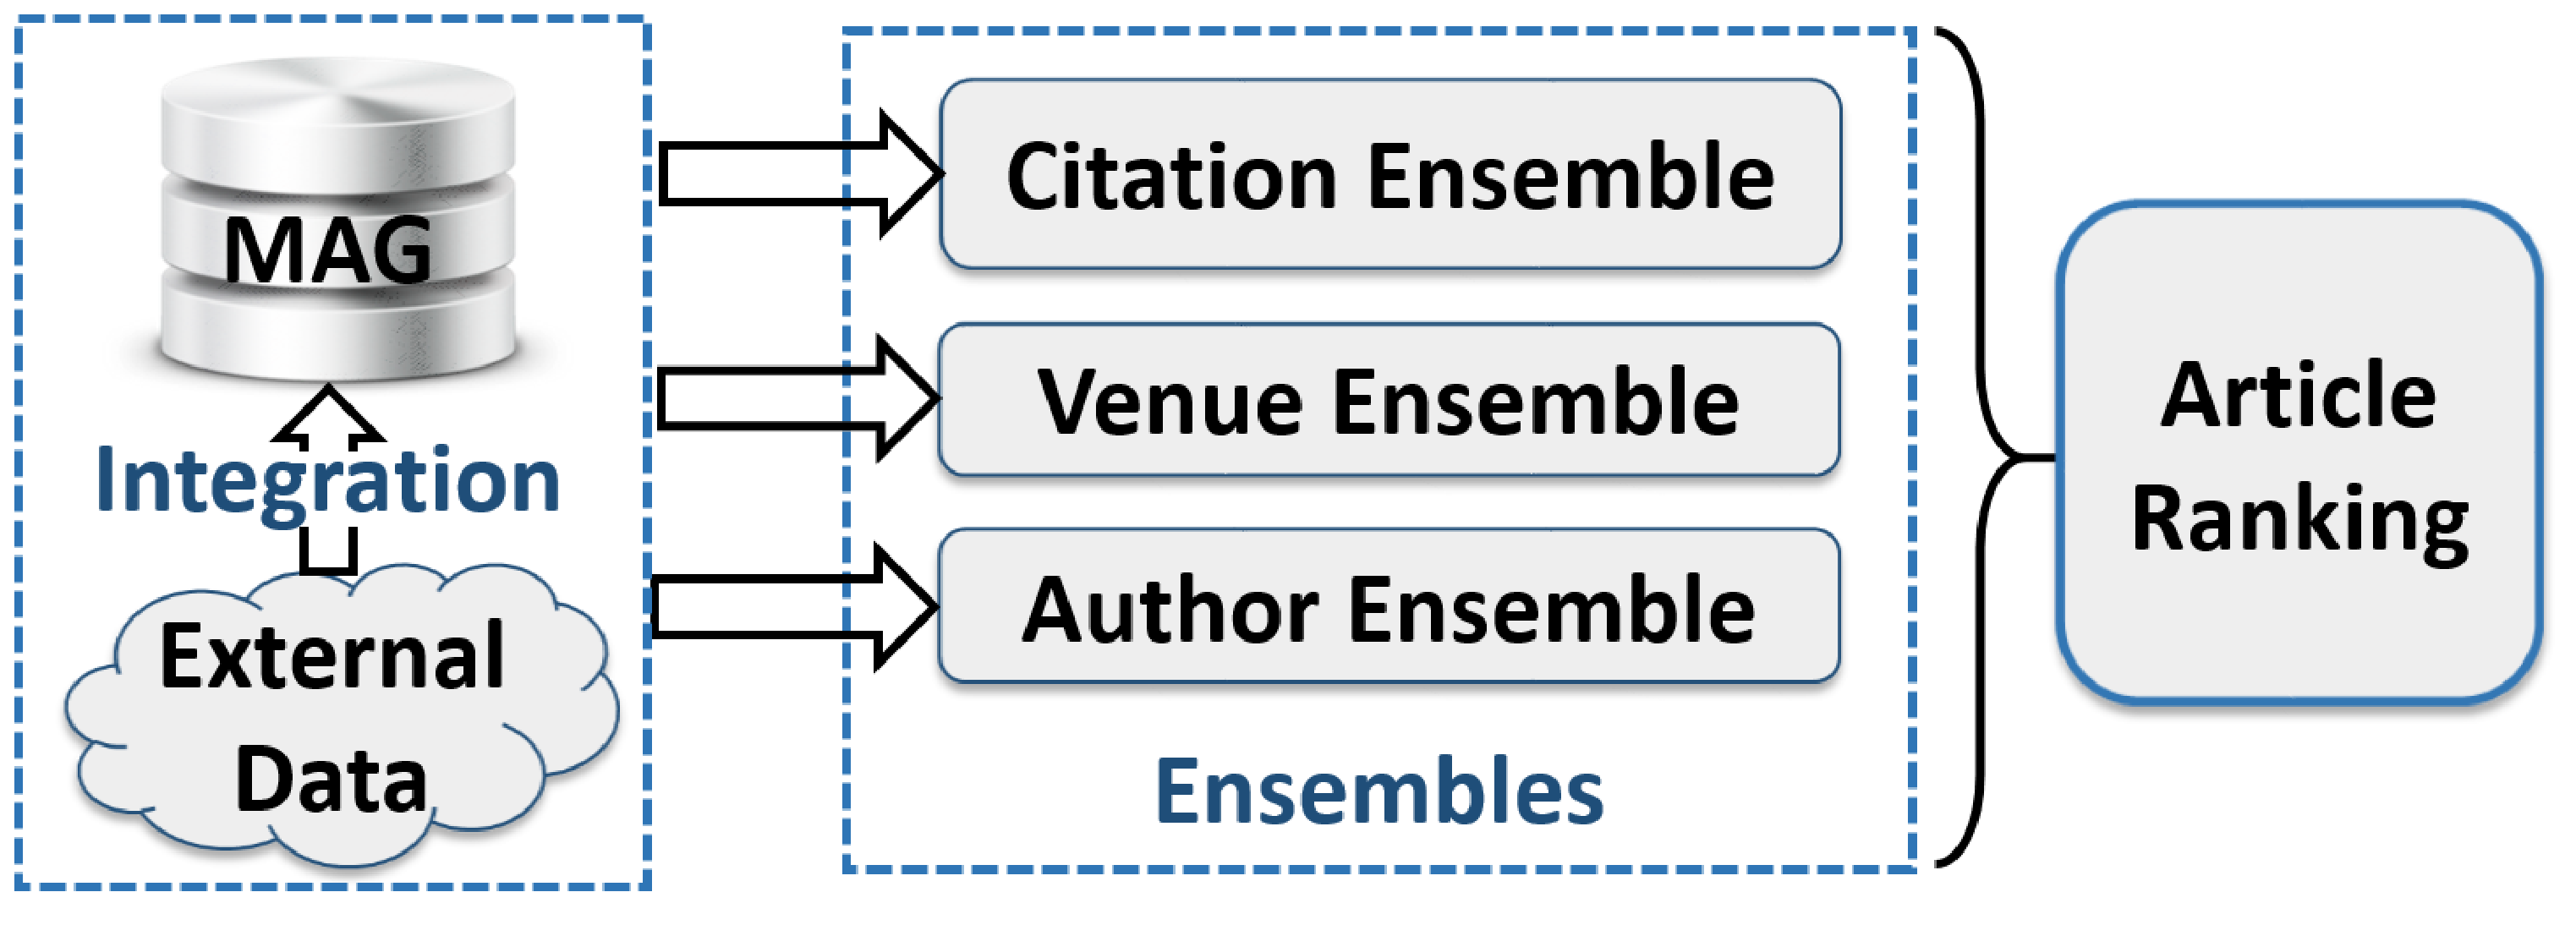
\includegraphics[scale=0.15]{fig/framework.eps}
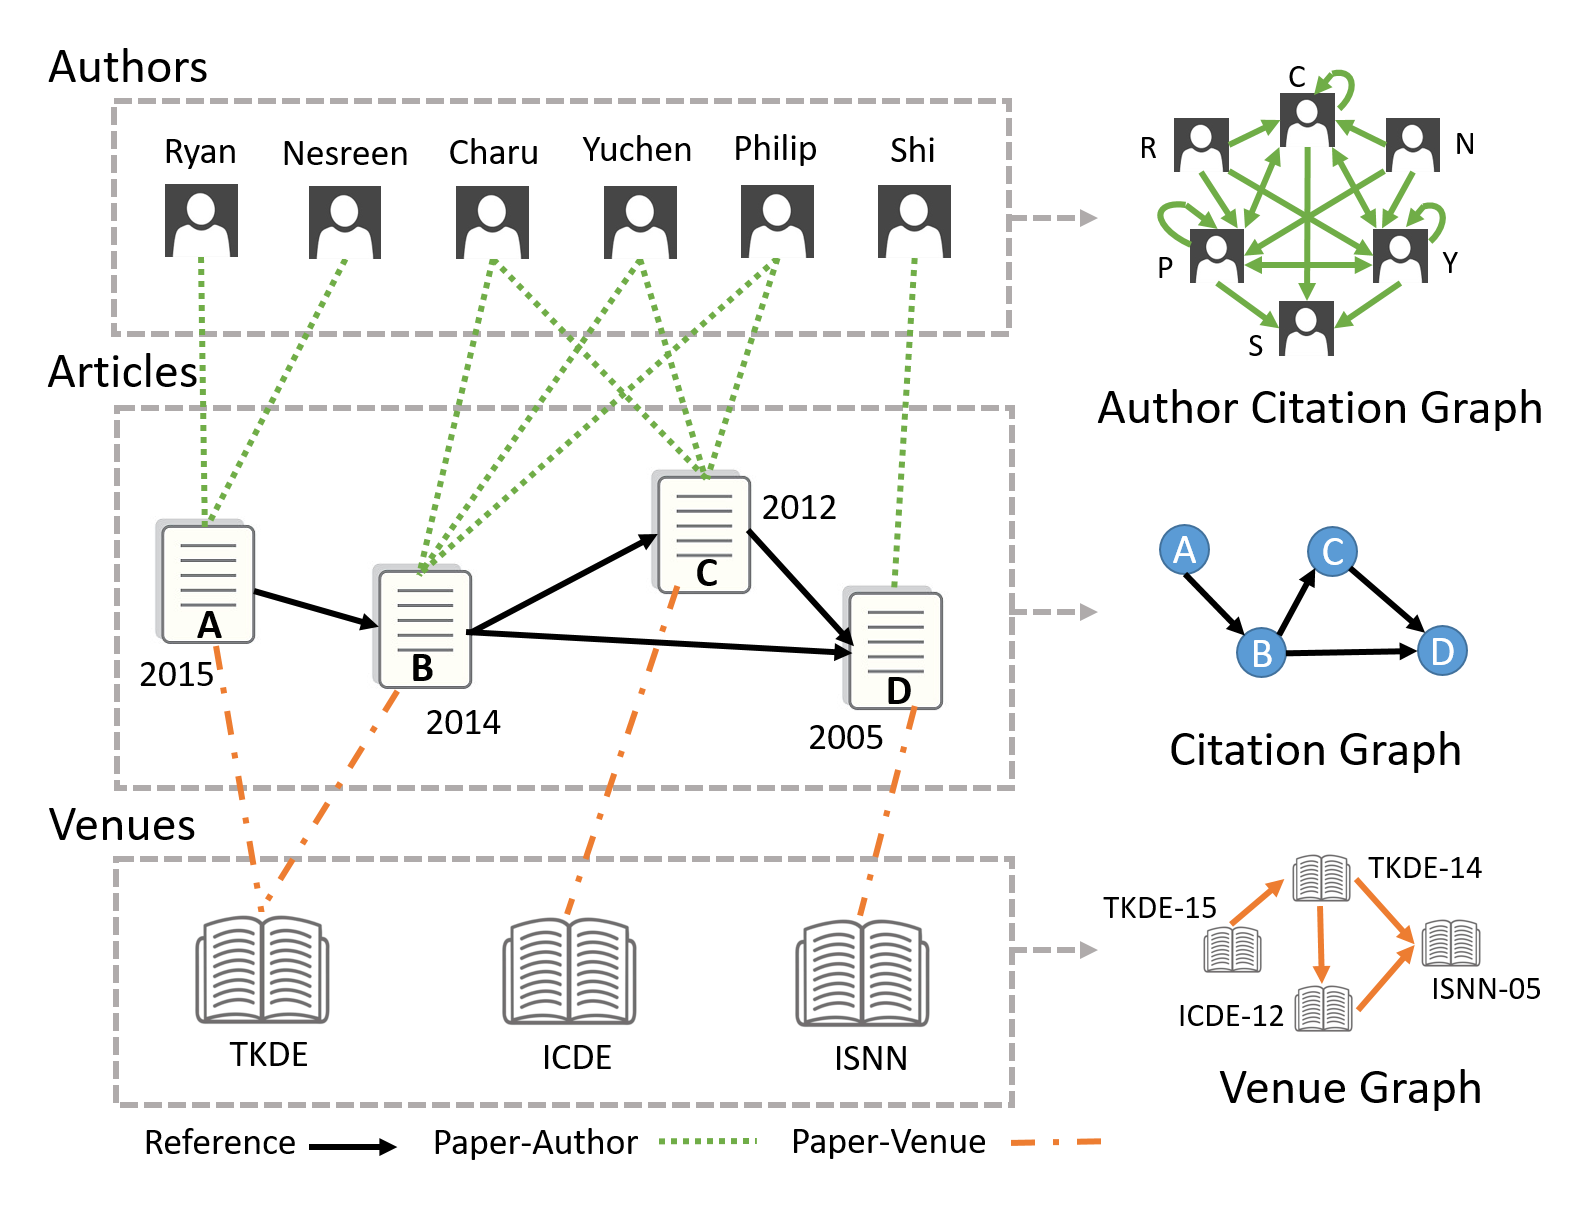
\includegraphics[scale=0.35]{fig/example-graph.eps}
\vspace{-1ex}
\caption{\small An example of graph generation} \label{fig-example-graph}
\vspace{-3ex}
\end{figure}

\begin{figure}[tb!]
\centering
%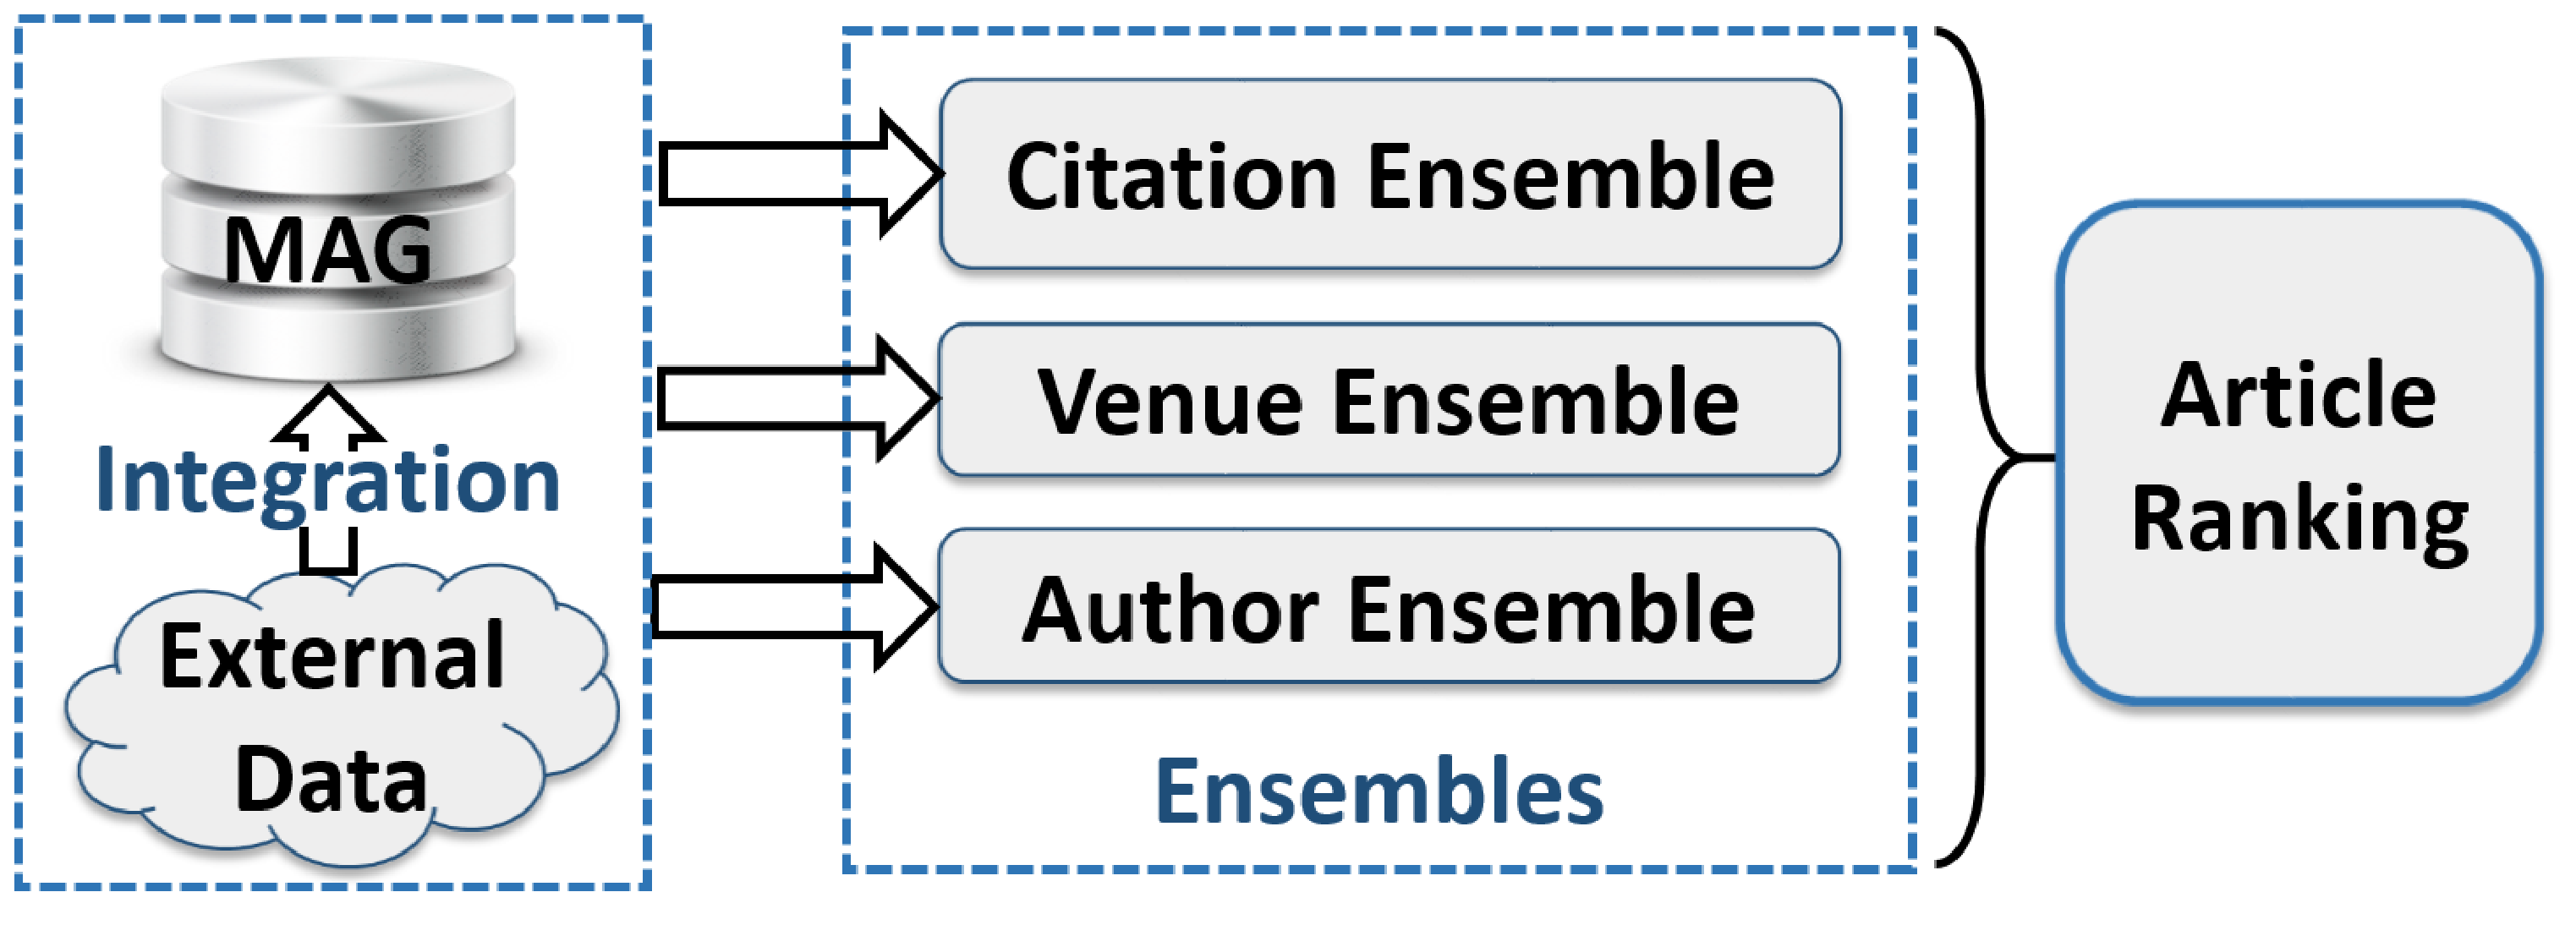
\includegraphics[scale=0.15]{fig/framework.eps}
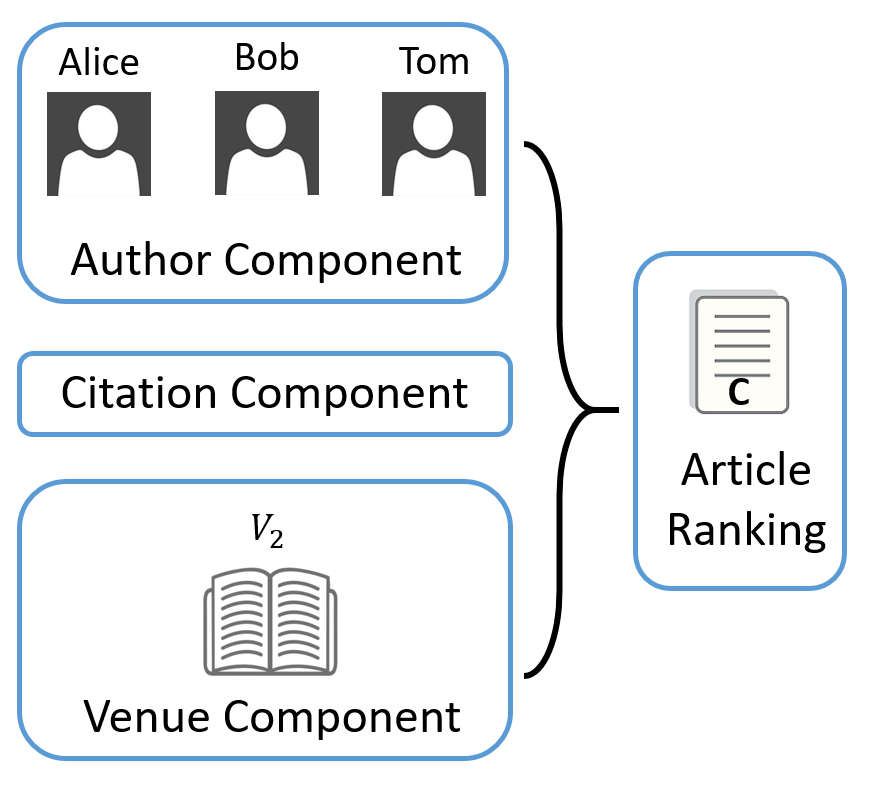
\includegraphics[scale=0.35]{fig/example-ranking.eps}
\vspace{-1ex}
\caption{\small An example of ranking model \ensemblerank} \label{fig-example-model}
\vspace{-3ex}
\end{figure}

%In our model, the importance of scholarly articles is defined as a combination of the prestige and popularity of its associated articles, venues and authors. Intuitively, prestige favors those with many citations soon after the publication of articles for citation component or associated articles for venue and author components, and popularity favors those with recent citations. Both prestige and popularity capture the temporal nature of entities in scholarly data.
In our model, the importance is defined as a combination of the prestige and popularity. Intuitively, prestige favors those with many citations soon after the publication of articles or associated articles of venues and authors, and popularity favors those with recent citations. Both prestige and popularity capture the temporal nature of entities. %in scholarly data.

Our ranking model \ensemblerank,  illustrated in Fig.~\ref{fig-rankmodel}, assembles the importance of article, venue and author entities for scholarly article ranking, which is computed by the citation, venue and author components, respectively.
%
We next introduce the details of the three components.


\begin{example} \label{eg-layer-dag}
Figure~\ref{fig-example-graph} illustrates an example of graph generation. We choose four articles of real-life data to show how to generate the citation graph, venue graph and author citation graph while the original academic graph data only has citation information, author-article relationships, article-venue relationships and time information of articles. As shown in Figure~\ref{fig-example-graph}, the articles A, B, C and D represent "Role Discovery in Networks", "On the Use of Side Information for Mining Text Data", "On Text Clustering with Side Information" and "Efficient streaming text clustering", respectively. We next introduce the details of graph generation.

The citation graph is constructed using the citation information such that each node denotes an individual article and the edge $(A,B)$ denotes that article A have cited article B. The venue graph is constructed using the citation information among venues. As shown in Figure~\ref{fig-example-graph}, each node denotes a venue in a specific year such that TKDE-14 and TKDE-15 are two different nodes. Further, each edge denotes that there are citations between the articles published in the two venues. The author citation graph is constructed using the citation information among authors. As shown in Figure~\ref{fig-example-graph}, the article citation between article A and article B will generate 6 different edges in author citation graph, which makes it much more complicated than citation graph. As a result, the citation graph of 4 articles and 4 edges have generated a author citation graph of 6 nodes and 18 edges (the bidirectional arrow denotes two edges) although the article B and article C have shared same authors.

\end{example}

\begin{example} \label{eg-layer-dag}
Figure~\ref{fig-example-model} illustrates an example of article ranking model. Consider an article $v$ published by authors $t$ and $u$ in venue $k$. 

\end{example}


   %%use this one for appendix


\eat{%%%%%%%%%%%%EAT
\stitle{Acknowledgments}.
This work is supported in part by  973 program ({\small No. 2014CB340300}), NSFC ({\small No. 61322207\&61421003}),  Special Funds of Beijing Municipal Science \& Technology Commission, and MSRA Collaborative Research Program. We also thank Liang Duan, Niannian Wu and Dr. Xuelian Lin for their support.
}%%%%%%%%%%%%%%%%EAT


%
% The following two commands are all you need in the
% initial runs of your .tex file to
% produce the bibliography for the citations in your paper.

%\newpage
%\clearpage
\balance

\bibliographystyle{IEEEtran}
\begin{small}
\bibliography{paper}
\end{small}

%\bibliographystyle{ACM-Reference-Format}
%\bibliography{paper}

%APPENDICES are optional
%\balancecolumns

\newpage
\clearpage

\section*{APPENDIX A: Proofs}
\label{sec-proof}


\subsection*{1. Proof of Corollary \ref{prop-prscc}}
The vector $PR$ returned by~\twprscc converges such that $||PR-PR^*||_1 < \epsilon$ given the convergent vector $PR^*$.

\vspace{.5ex}
\begin{proofS}
%By lemma~\ref{prop-converg}, we know that TWPageRank converges on venue graphs.
We first prove that the sum of changes after another iteration from $PR$ is smaller than $\epsilon$, \ie $||PR'-PR||_1 < \epsilon$ where $PR'=d M^T\cdot PR + \frac{1-d}{n} e$, and then prove that $||PR^*-PR||_1$ is smaller than $||PR'-PR||_1$.
%the sum of changes.

Consider $scc_1$, $\dots$, $scc_m$ of the (citation or venue) graph $G$ such that $v_1'/\dots$ $/v_m'$ is indeed a valid topological order of the block-wise graph $G'$ of $G$, where %$m$ is the number of \sccs in $G$ and
$v_k'$ ($k\in [1,m]$) is the corresponding node of $scc_k$ in $G'$.

Let $PR_k$ and $PR_k^-$ be the current and the previous TWPageRank vectors of nodes in $scc_k$ produced
by \twprscc, and $PR_k'$ be the TWPageRank vector of nodes in $scc_k$ extracted from $PR'$.
Further let $\Delta_k=PR_k-PR^-_k$ and we have:
$\sum_{k=1}^m ||\Delta_k||_1 < \epsilon$.
%
Consider $M_{ij}$ ($i,j\in[1,m]$), the submatrix of $M$ denoting the transition probability from nodes in $scc_i$ to nodes in $scc_j$. We have $M_{ij}=\bf{0}$ when $i>j$, since there exists no edges from nodes in $scc_i$ to $scc_j$. And, hence, $PR_k$ and $PR_k'$ are updated as:

\vspace{-1ex}
\begin{small}
\begin{equation*}
\begin{split}
PR_k=&\frac{1-d}{n} e_k+ d \sum_{j=1}^{k-1} M_{jk}^T PR_j + d M_{kk}^T PR_k^-,\\
PR_k'=&\frac{1-d}{n}  e_k+ d \sum_{j=1}^{k-1} M_{jk}^T PR_j + d M_{kk}^T PR_k,
\end{split}
\end{equation*}
\end{small}
\noindent
respectively, where $e_k=[1]_{|scc_k|\times 1}$.
%, and, obviously, $\Delta_k^+=PR_k^+-PR_k=d M_{kk}^T \Delta_k^-$.


Given these, the sum of changes between $PR'$ and $PR$ is:

\vspace{-1ex}
\begin{small}
\begin{equation*}
\begin{split}
||PR'-PR||_1 & =\sum_{k=1}^m ||PR_k'-PR_k||_1 = \sum_{k=1}^m ||d M_{kk}^T \Delta_k||_1 \\
& \le d\sum_{k=1}^m ||\Delta_k||_1 < \epsilon,
\end{split}
\end{equation*}
\end{small}
\noindent
based on the fact that the row sums of $M_{kk}$ are always $\le 1$. %less than or equal to 1.

Moreover, $||PR'-PR||_1 = ||PR' - PR^* + PR^* -PR||_1 = ||d M^T (PR-PR^*)||_1 + ||PR-PR^*||_1<\epsilon$, which gives $||PR-PR^*||_1<\epsilon$ and proves the conclusion.
\end{proofS}

\subsection*{2. Proof of Proposition \ref{lemma-inc-topo}}
$O^+=\Delta O/O$ is indeed a valid topological order of the block-wise graph of $G^+$.

\vspace{.5ex}
\begin{proofS}
Let $G'_\Delta(V'_\Delta, E'_\Delta)$ be the block-wise graph of $G^+[\Delta V]$; further let $E'_c$ denote the set of crossing edges from $V'_\Delta$ to $V'$.
It suffices to show that for each $(u,v)\in E'\cup E'_\Delta \cup E'_c$, $u$ comes before $v$ in $O^+$,
which obviously holds (a) for  $E'\cup E'_\Delta$ as $O$ and $\Delta O$ are topological orders of $G'$ and $G'_\Delta$, respectively, and (b) for $E_{c}'$ as nodes in $G'_\Delta$ come before nodes in $G'$.
\end{proofS}



\subsection*{3. Proof of Theorem \ref{lemma-subgraphA}}
The TWPageRank vector $PR^+$ returned by~\inctwprscc converges such that $||PR^+-PR^{*}||_1 < \epsilon$, where $PR^{*}$ is the convergent TWPageRank vector.

\vspace{.5ex}
\begin{proofS}
Assume a topological order $v_1'/\dots/v_{l}'$ of block-wise graph $G^+{'}$ where $l=|O^+|$. We prove that the sum of change of $PR^+(v)$ where $v\in scc_k$ is no more than $\epsilon\cdot\frac{|scc_k|}{|V^+|}$ for $scc_k$ corresponding to $v_k'$ ($k\in [1,l]$) by induction. Note that it obvious holds for $scc_k$ belonging to $G_B$ and $G_C$ by algorithm~\inctwprscc.

\noindent(1) When $k=1$, it holds since $scc_1$ belongs to $G_C$;

\noindent(2) Assume that it holds when $1\le k\le q$. We then show that it also holds for $k=q+1$. It suffices to show the case when $scc_k$ belongs to $G_A$. Recall that:

\vspace{-1ex}
\begin{scriptsize}
\begin{equation*}
\begin{split}
PR(v) & =  d \sum_{(u,v)\in E_i} M_{u,v} PR(u) + d \sum_{(u,v)\in E_a} M_{u,v} PR(u) +  \frac{1-d}{n},\\
PR^+(v) & =  d \sum_{(u,v)\in E^+_i} M^+_{u,v} PR^+(u) + d \sum_{(u,v)\in E^+_a} M^+_{u,v} PR^+(u) +  \frac{1-d}{n^+}.
\end{split}
\end{equation*}
\end{scriptsize}
\noindent
Consider $scc_k$ belonging to $G_A$ and node $v\in scc_k$. We have $\{(u,v)|(u,v)\in E_i\}$ = $\{(u,v)|$ $(u,v)\in E^+_i\}$, $\{(u,v)|(u,v)\in E_a\}$ = $\{(u,v)|(u,v)\in E^+_a\}$ and $M_{u,v}=M^+_{u,v}$ when $(u,v)\in E_i\cup E_a$. Also note that $PR^+(u)=\frac{n}{n^+}PR(u)$ when $(u,v)\in E_a$ according to algorithm~\inctwprscc. Let $PR_{k,0}$, $PR_{k,1}$, $\dots$, $PR_{k,t}$ be the convergent sequence of TWPageRank vectors for $scc_k$ computed by algorithm \twprscc on $G$. Then $\frac{n}{n^+}PR_{k,0}$, $\frac{n}{n^+}PR_{k,1}$, $\dots$, $\frac{n}{n^+}PR_{k,t}$ is a valid convergent sequence of TWPageRank vectors for $scc_k$ computed by algorithm \inctwprscc on $G^+$ given the initial TWPageRank vector $\frac{n}{n^+}PR_{k,0}$.
Hence, the sum of changes of $PR^+(v)$ where $v\in scc_k$ is $\frac{n}{n^+}||PR_{k,t}-PR_{k,t-1}||_1 < \epsilon\cdot\frac{|scc_k|}{|V^+|}$.

Combining with Corollary \ref{prop-prscc}, we have the conclusion.
\end{proofS}


\section*{APPENDIX B: Detailed of Model}
\label{sec-exp-app}

\subsection{Ranking with Importance Assembling}
\label{subsec-ensemble}

\begin{figure}[tb!]
\centering
%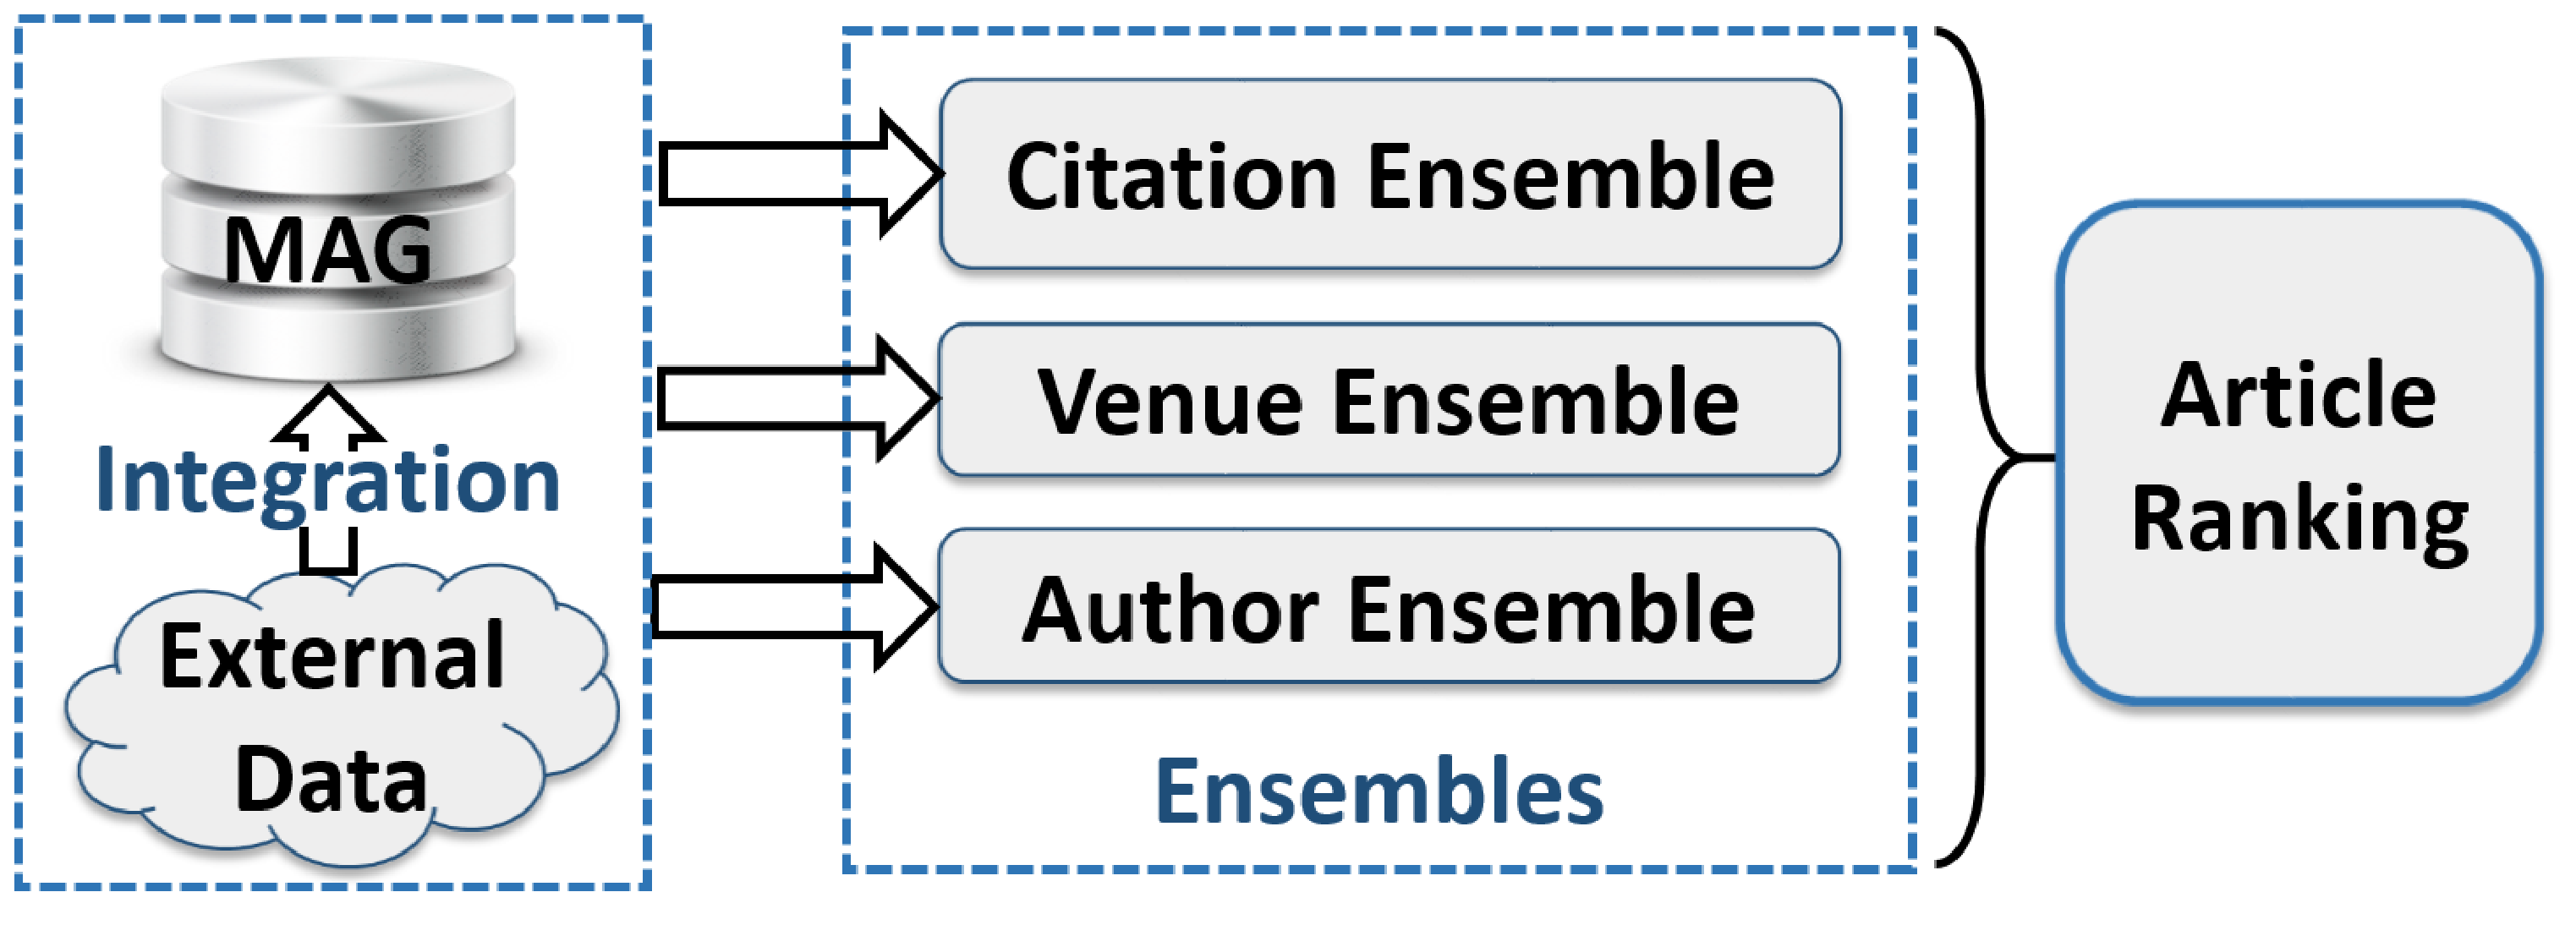
\includegraphics[scale=0.15]{fig/framework.eps}
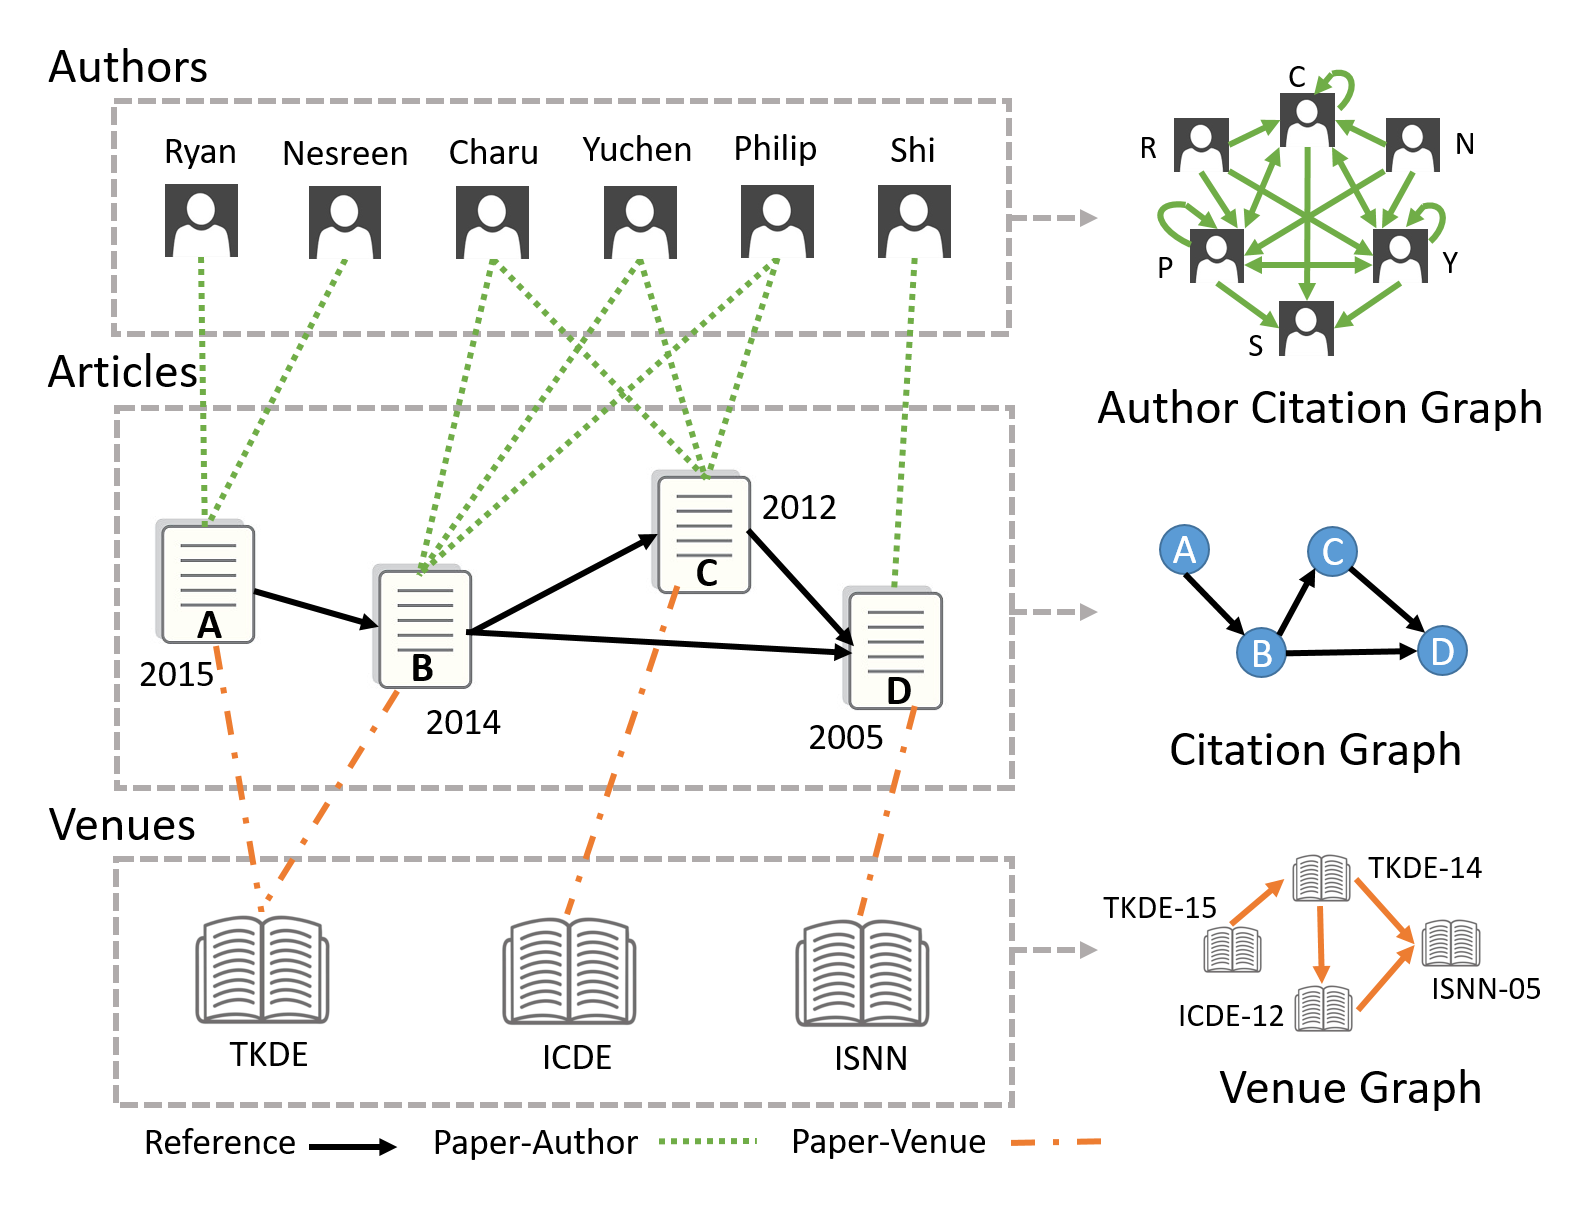
\includegraphics[scale=0.35]{fig/example-graph.eps}
\vspace{-1ex}
\caption{\small An example of graph generation} \label{fig-example-graph}
\vspace{-3ex}
\end{figure}

\begin{figure}[tb!]
\centering
%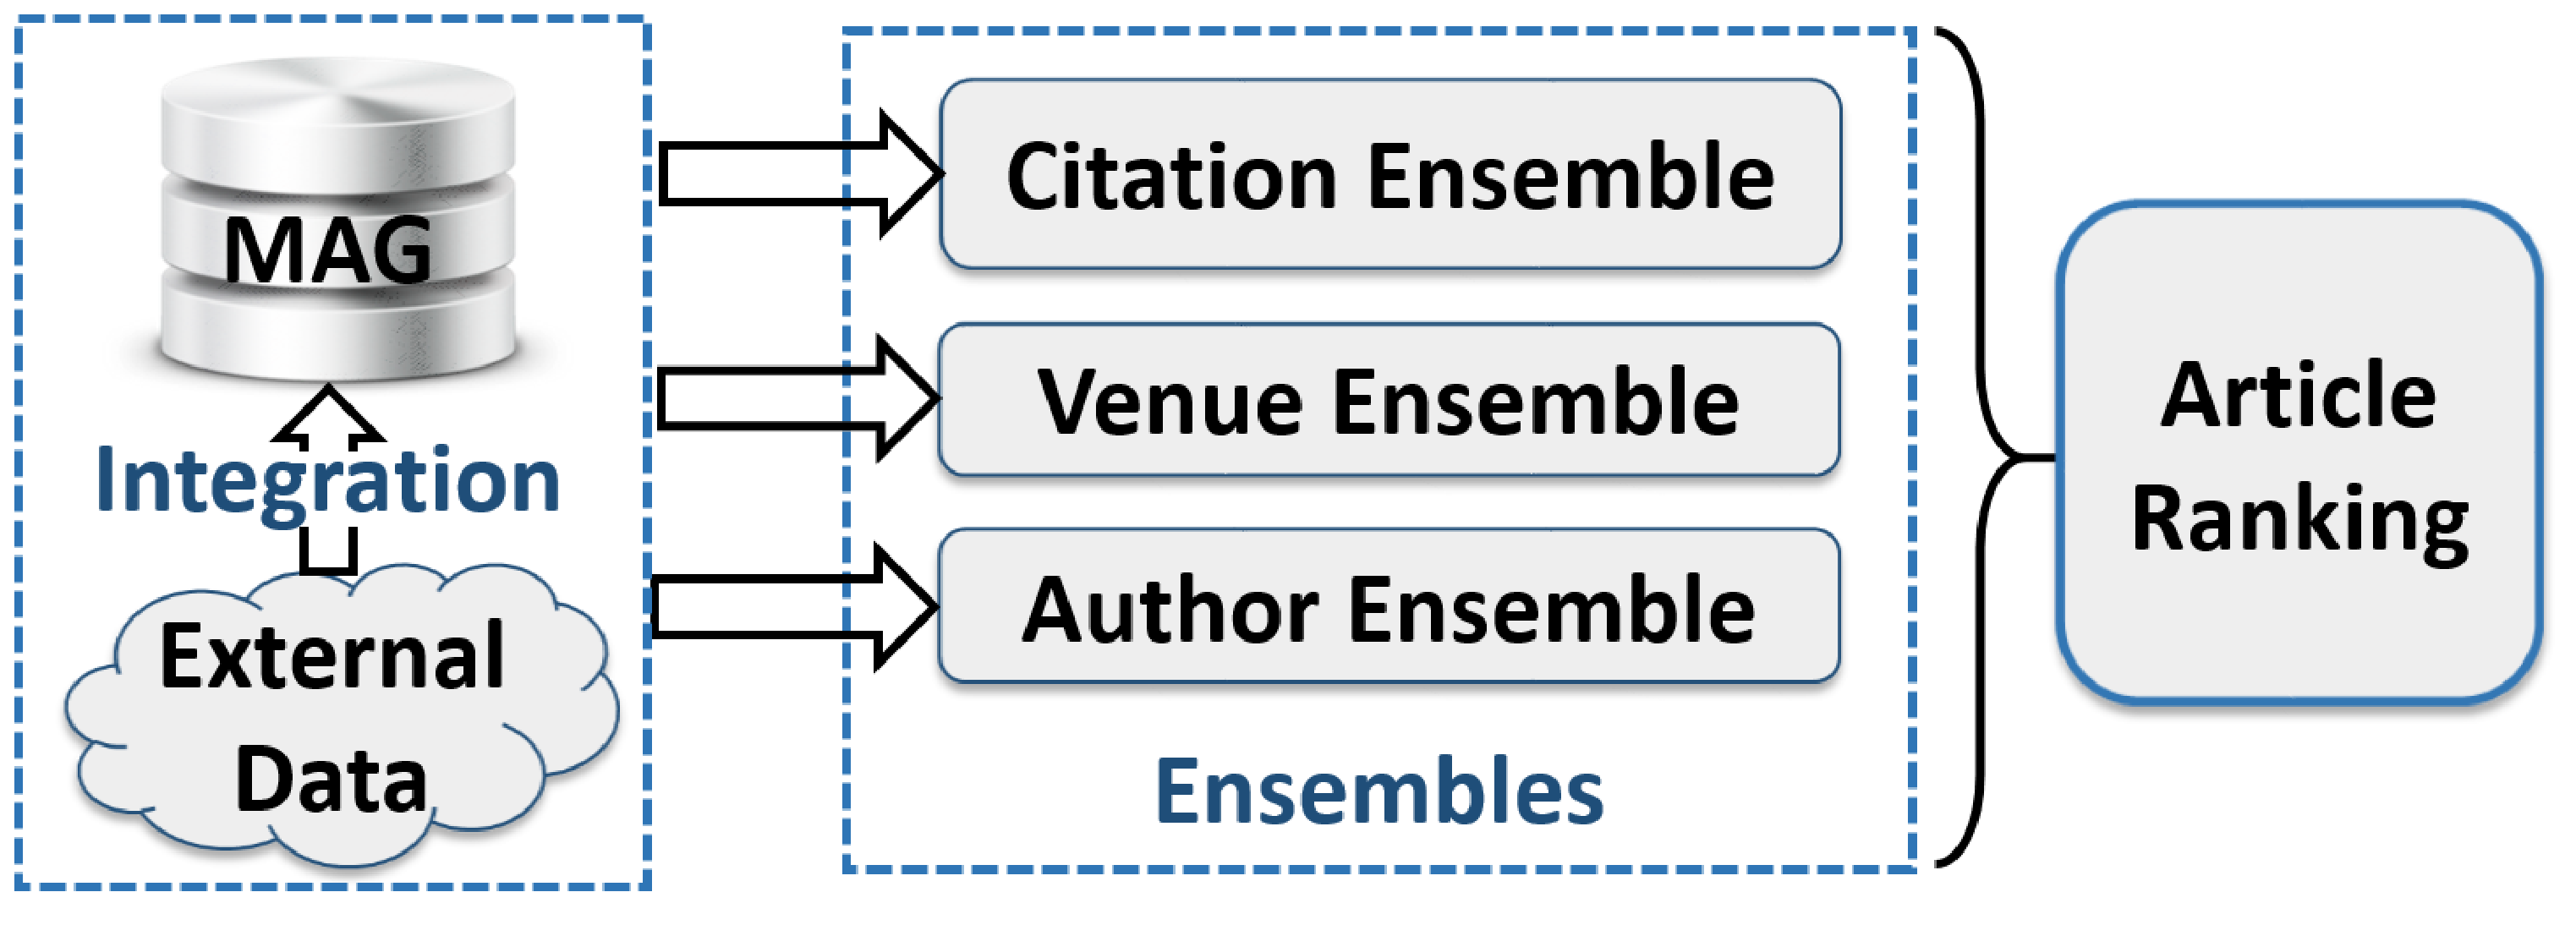
\includegraphics[scale=0.15]{fig/framework.eps}
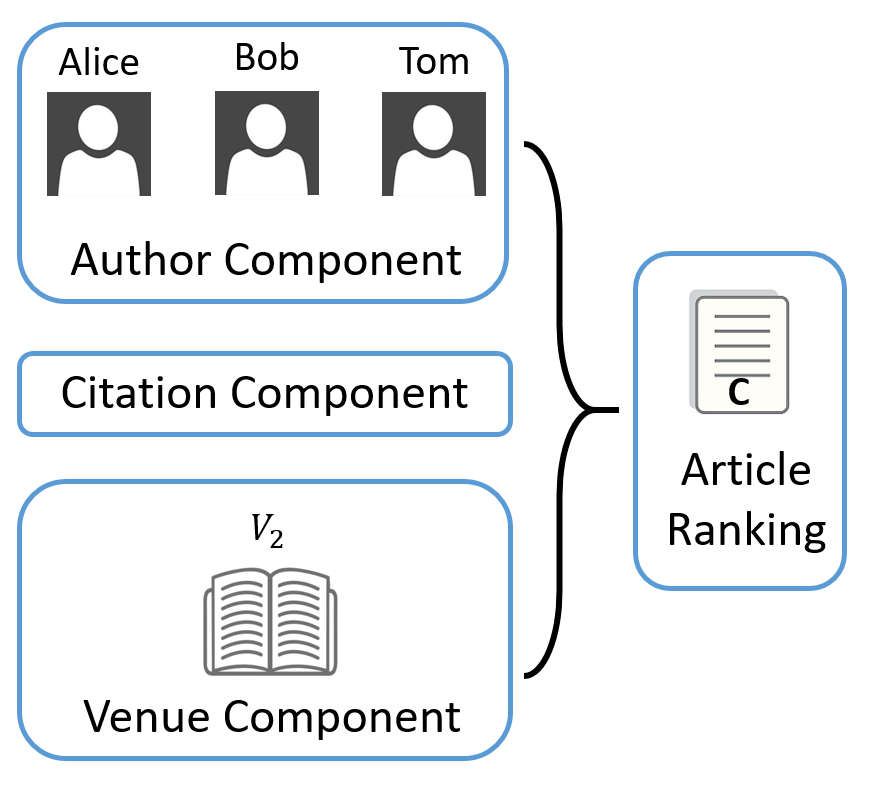
\includegraphics[scale=0.35]{fig/example-ranking.eps}
\vspace{-1ex}
\caption{\small An example of ranking model \ensemblerank} \label{fig-example-model}
\vspace{-3ex}
\end{figure}

%In our model, the importance of scholarly articles is defined as a combination of the prestige and popularity of its associated articles, venues and authors. Intuitively, prestige favors those with many citations soon after the publication of articles for citation component or associated articles for venue and author components, and popularity favors those with recent citations. Both prestige and popularity capture the temporal nature of entities in scholarly data.
In our model, the importance is defined as a combination of the prestige and popularity. Intuitively, prestige favors those with many citations soon after the publication of articles or associated articles of venues and authors, and popularity favors those with recent citations. Both prestige and popularity capture the temporal nature of entities. %in scholarly data.

Our ranking model \ensemblerank,  illustrated in Fig.~\ref{fig-rankmodel}, assembles the importance of article, venue and author entities for scholarly article ranking, which is computed by the citation, venue and author components, respectively.
%
We next introduce the details of the three components.


\begin{example} \label{eg-layer-dag}
Figure~\ref{fig-example-graph} illustrates an example of graph generation. We choose four articles of real-life data to show how to generate the citation graph, venue graph and author citation graph while the original academic graph data only has citation information, author-article relationships, article-venue relationships and time information of articles. As shown in Figure~\ref{fig-example-graph}, the articles A, B, C and D represent "Role Discovery in Networks", "On the Use of Side Information for Mining Text Data", "On Text Clustering with Side Information" and "Efficient streaming text clustering", respectively. We next introduce the details of graph generation.

The citation graph is constructed using the citation information such that each node denotes an individual article and the edge $(A,B)$ denotes that article A have cited article B. The venue graph is constructed using the citation information among venues. As shown in Figure~\ref{fig-example-graph}, each node denotes a venue in a specific year such that TKDE-14 and TKDE-15 are two different nodes. Further, each edge denotes that there are citations between the articles published in the two venues. The author citation graph is constructed using the citation information among authors. As shown in Figure~\ref{fig-example-graph}, the article citation between article A and article B will generate 6 different edges in author citation graph, which makes it much more complicated than citation graph. As a result, the citation graph of 4 articles and 4 edges have generated a author citation graph of 6 nodes and 18 edges (the bidirectional arrow denotes two edges) although the article B and article C have shared same authors.

\end{example}

\begin{example} \label{eg-layer-dag}
Figure~\ref{fig-example-model} illustrates an example of article ranking model. Consider an article $v$ published by authors $t$ and $u$ in venue $k$. 

\end{example}


   %%use this one for appendix

\end{document}
